\documentclass[8pt, a4paper, twocolumn, twoside]{extarticle}

\usepackage{extsizes} % Smaller text
\usepackage[italian]{babel} % Italian support
\usepackage{amsmath,amsfonts,amssymb,mathtools,calrsfs}
\usepackage{bm} % Bold math
\usepackage[utf8]{inputenc} % Accented letters
\usepackage[medium]{titlesec} % Smaller section's font
\usepackage[pdftex,dvipsnames,table]{xcolor} % Colors for text
\usepackage{array} % For better tables
\usepackage{parskip} % To avoid indentation
\usepackage{textcomp} % To have \textcelsius and other symbols
\usepackage{multirow} % For nicer tables with split rows/columns
\usepackage{multicol}
\usepackage{cancel} % Cacelled equations and simplifications
\usepackage{xargs} % Allows for multiple arguments commmands
\usepackage{enumitem} % For more flexibility on lists
\usepackage{xtab, booktabs, array}
\usepackage[labelformat=empty]{caption}

\usepackage[showframe=false, top=1cm, bottom=1.5cm, left=1.5cm, right=1.5cm]{geometry}

\usepackage[colorinlistoftodos,prependcaption,textsize=tiny]{todonotes}
% Some useful TODO commands
\newcommandx{\unsure}[2][1=]{\todo[linecolor=red,backgroundcolor=red!25,bordercolor=red,#1]{#2}}
\newcommandx{\change}[2][1=]{\todo[linecolor=blue,backgroundcolor=blue!25,bordercolor=blue,#1]{#2}}
\newcommandx{\info}[2][1=]{\todo[linecolor=OliveGreen,backgroundcolor=OliveGreen!25,
bordercolor=OliveGreen,#1]{#2}}
\newcommandx{\improvement}[2][1=]{\todo[linecolor=Plum,backgroundcolor=Plum!25,
bordercolor=Plum,#1]{#2}}
\newcommandx{\thiswillnotshow}[2][1=]{\todo[disable,#1]{#2}}

\setlength{\marginparwidth}{2cm} % For better TODO's display

\usepackage{hyperref}
\hypersetup{
  colorlinks,
  citecolor=black,
  filecolor=black,
  linkcolor=blue,
  urlcolor=black
}
\usepackage[all]{hypcap} % To fix caption loading of hyperref

\usepackage{tikz}
\usetikzlibrary{
  arrows,
  decorations,
  decorations.markings,
  decorations.pathmorphing,
  calc,
  intersections,
  shapes.geometric,
  shapes.misc
}
\tikzset{>=stealth}
\usepackage[siunitx]{circuitikz}
% http://texdoc.net/texmf-dist/doc/latex/circuitikz/circuitikzmanual.pdf
\usepackage{tikz-3dplot}

% \usepackage{showframe} % For spaces
% \usepackage{showkeys} % For labels and references.

\setcounter{secnumdepth}{0} % sections are level 1
\setcounter{tocdepth}{3}

\DeclarePairedDelimiter\norm{\lVert}{\rVert} % ||v||
\DeclarePairedDelimiter\abs{\lvert}{\rvert} % |v|

\newcommand\markangle[7][red]{% [color] origin A B radius radiusmark mark
  % fill red circle
  \begin{scope}
    \path[clip] (#2) -- (#3) -- (#4);
    \fill[color=#1,fill opacity=0.5,draw=#1,name path=circle]
    (#2) circle (#5);
  \end{scope}
  % middle calculation
  \path[name path=line one] (#2) -- (#3);
  \path[name path=line two] (#2) -- (#4);
  \path[%
  name intersections={of=line one and circle, by={inter one}},
  name intersections={of=line two and circle, by={inter two}}
  ] (inter one) -- (inter two) coordinate[pos=.5] (middle);
  % put mark
  \node at ($(#2)!#6!(middle)$) {#7};
}

\def\mathcolor#1#{\@mathcolor{#1}}
\def\@mathcolor#1#2#3{%
  \protect\leavevmode
  \begingroup
  \color#1{#2}#3%
  \endgroup
}

% For better visual in tables
\renewcommand*{\arraystretch}{2}
% To center with m{}
\usepackage{array}
\newcolumntype{M}[1]{>{\centering\arraybackslash}m{#1}}

\newcommand{\divisor}{\rule{8.7cm}{0.4pt}}

% For an older but clearer root. Still \oldsqrt is valid
\usepackage{letltxmacro}
\makeatletter
\let\oldr@@t\r@@t
\def\r@@t#1#2{%
  \setbox0=\hbox{$\oldr@@t#1{#2\,}$}\dimen0=\ht0
  \advance\dimen0-0.2\ht0
  \setbox2=\hbox{\vrule height\ht0 depth -\dimen0}%
{\box0\lower0.4pt\box2}}
\LetLtxMacro{\oldsqrt}{\sqrt}
\renewcommand*{\sqrt}[2][\ ]{\oldsqrt[#1]{#2} }
\makeatother

% Matrix spacing
\makeatletter
\renewcommand*\env@matrix[1][\arraystretch]{%
  \edef\arraystretch{#1}%
  \hskip -\arraycolsep
  \let\@ifnextchar\new@ifnextchar
\array{*\c@MaxMatrixCols c}}
\makeatother

\newcommand\twodigits[1]{%
  \ifnum#1<10 0\number#1 \else #1\fi
}

\usepackage[yyyymmdd]{datetime}
\renewcommand{\dateseparator}{-}

\usepackage{fancyhdr}
\pagestyle{fancy}
\fancyhead{} % clear all header fields
\renewcommand{\headrulewidth}{0pt} % no line in header area
\fancyfoot{} % clear all footer fields
\fancyfoot[LE,RO]{
  \thepage
}
\fancyfoot[RE,LO]{
  ``Fatti non foste a viver come bruti ma per seguir virtute e canoscenza'' - Dante Alighieri, 
  ``Inferno''
}
\fancypagestyle{firststyle}{
  \fancyhf{}
  %\fancyfoot[C]{\thepage}
  \fancyfoot[L]{
    Version 1.0.13 \today
  }
  \fancyfoot[R]{
    Copyright \copyright 2017--\the\year$\,$Cossu Davide
  }
}

\newcommand*\dif{\mathop{}\!\mathrm{d}}
\newcommand*\Dif{\mathop{}\!\mathrm{D}}
\newcommand*{\der}[2]{\frac{\dif #1}{\dif #2}}

\everymath{\displaystyle}

\begin{document}
\thispagestyle{firststyle}
\onecolumn
\begin{@twocolumnfalse}
  \clearpage
  \vspace*{\stretch{1.5}}
  \begin{center}
    \begin{figure*}[!h]
      \centering
      \captionsetup{justification=centering}
      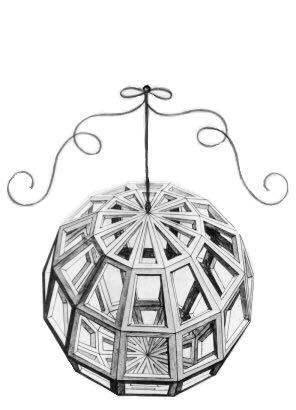
\includegraphics[scale=3]{colophon/daVinci}
      \caption{\textit{`La fisica è, tra tutte le scienze, la più fondamentale e completa,
          e ha avuto una profonda influenza. Studenti delle discipline più diverse si 
          ritrovano a doverla studiare a causa dell'importanza che riveste in tutti i 
        fenomeni.'}\\- Richard Feynman\\ [\baselineskip]
        \textit{`Causas rerum naturalium non plures admittiri debere, quam quo et vera 
      sint et earum ph\ae nomeni explicandis sufficiant.'}\\- Isaac Newton}
      \label{fig:deer}
    \end{figure*}
    \vspace{1cm}
    \begin{minipage}{.6\textwidth}				
      \begin{center}
        {\Huge\textbf{Formulario di Fisica}}\\\vspace{0.2cm}
        {\textbf{Davide Cossu, Stefano D'Agaro}}
      \end{center}
      \vspace{0.5cm}
      Questo è un formulario con le formule di fisica fatte durante i cinque anni 
      di un liceo scientifico con alcune spiegazioni teoriche, esercizi e suggerimenti.
    \end{minipage}
  \end{center}
  \vspace{\stretch{3}} % \vfill equivalent to \vspace{\fill}
  \clearpage
\end{@twocolumnfalse}

\twocolumn
{
  \hypersetup{linkcolor=black}
  \tableofcontents
}

\newpage
\textbf{Durante tutto il formulario, si userà il sistema internazionale di notazione, ovvero $.$ per 
separare interi da decimali e $,$ per separare le migliaia se necessario.}
\section{Costanti}
Qui verranno riportate le costanti usate nelle formule con relativo simbolo e unità di misura.

\tablefirsthead{\toprule Simbolo& Nome & Valore & Unità di misura \\ \midrule}
\tablehead{Simbolo& Nome & Valore & Unità di misura \\ \midrule}
\tablelasttail{\bottomrule}

\begin{center}
  \begin{xtabular}{c M{1.8cm} c M{1.5cm}}
    \label{tab:pi}
    $\pi$ & Pi greco & $3.14$ & /\\\midrule
    \label{tab:g} 
    $g$ & Accelerazione gravitazionale & $9.81$ & $\frac{\text{m}}{\text{s}^2}$\\ \midrule
    \label{tab:G} 
    $G$ & Costante di Gravitazione Universale & $6.67\cdot10^{-11}$ &		
    $\frac{\text{Nm}^2}{\text{kg}^2}$\\\midrule
    \label{tab:mT}
    $m_{\text{Terra}}$ & Massa della Terra & $5.9\cdot10^{24}$ & $kg$\\ \midrule
    \label{tab:rT}
    $r_{\text{Terra}}$ & Raggio della Terra & $6378$ & $m$\\ \midrule 
    \label{tab:patm} 
    \multirow{5}[1]{*}{$p_{atm}$} & \multirow{5}[1]{1.8cm}{\centering Pressione atmosferica} & 
    $1$ & $\text{atm}$\\
        && $1.01\cdot10^{5}$ & $\text{Pa}$\\ 
        && $760$ & $\text{mm}\,\text{Hg}$\\
        && $1.01\cdot10^{5}$ & $\frac{\text{N}}{\text{m}^2}$\\
        && $1$ & $\text{bar}$\\ \midrule
    \label{tab:Na} 
    $N_A$ & Numero di Avogadro & $6.02\cdot10^{23}$ & /\\ \midrule
    \label{tab:Vm} 
    $V_m$ & Volume occupato da Gas in STP & $22.4$ & $\text{l}$\\ \midrule
    \label{tab:R} 
    \multirow{2}[1]{*}{$R$} & \multirow{2}[1]{1.8cm}{\centering Costante universale dei Gas} & 
    $0.0821$ & $\frac{\text{l}\cdot\text{atm}}{\text{nK}}$\\
             && $8.31$ & $\frac{\text{J}}{\text{nK}}$\\ \midrule
    \label{tab:cH2O} 
    \multirow{2}[1]{*}{$c_{H_2O}$} & \multirow{2}[1]{1.8cm}{\centering Calore specifico 
    dell'acqua} & $4.186\cdot10^3$ & $\frac{\text{C}}{\text{kg}\cdot\text{K}}$\\
                && $1$ & $\frac{\text{cal}}{\text{g}\cdot\text{K}}$\\\midrule
    \label{tab:cfa} 
    $\lambda_f$ & Calore di fusione dell'acqua & $3.335\cdot10^5$ & 
    $\frac{\text{J}}{\text{Kg}}$\\\midrule
    \label{tab:cva} 
    $\lambda_v$ & Calore di vaporizzazione dell'acqua & $2.257\cdot10^6$ &
    $\frac{\text{J}}{\text{Kg}}$\\\midrule
    \label{tab:kB} 
    $k_B$ & Costante di Boltzman & $1.381\cdot10^{-23}$ & 
    $\frac{\text{J}}{\text{K}}$\\ \midrule
    \label{tab:c} 
    $c$ & Velocità della luce & $3\cdot10^8$ & $\frac{\text{m}}{\text{s}}$\\\midrule
    \label{tab:I0} 
    $I_0$ & Soglia di udibilità & $10\cdot10^{-12}$ & 
    $\frac{\text{W}}{\text{m}^2}$\\ \midrule
    \label{tab:Im} 
    $I_m$ & Soglia del dolore & $1$ & $\frac{\text{W}}{\text{m}^2}$\\ \midrule
    \label{tab:vs} 
    $v$ & Velocità del suono & $343$ & $\frac{\text{m}}{\text{s}}$\\ \midrule
    \label{tab:e0} 
    $\varepsilon_0$& Costante dielettrica nel vuoto&$8.9\cdot10^{-12}$&
    $\dfrac{\text{C}^2}{\text{N}\cdot\text{m}^2}$\\ \midrule
    \label{tab:k0}
    $k_0$ & Costante di Coulomb & $9\cdot10^9$ & 
    $\frac{\text{N}\cdot\text{m}^2}{\text{C}^2}$\\ \midrule
    \label{tab:e-} 
    $e^{-}$ & Carica di un elettrone & $-1.60\cdot10^{-19}$ & $\text{C}$\\ \midrule
    \label{tab:me-} 
    $m_{e^{-}}$ & Massa di un elettrone & $9.11\cdot10^{-28}$ & $\text{kg}$\\\midrule
    \label{tab:u} 
    $u$ & Unità di massa atomica & $1.7\cdot10^{-7}$ & $\text{kg}$\\\midrule
    \label{tab:mu0} 
    $\mu_0$ & Permeabilità magnetica nel vuoto & $4\pi\cdot10^{-7}$ & 
    $\frac{\text{N}}{\text{A}^2}$\\
    \midrule
  \end{xtabular}
\end{center}

\newpage
\section{Unità di misura}
\tablefirsthead{\toprule Grandezza & Nome & Simbolo & Definizione \\ \midrule}
\tablehead{Grandezza & Nome & Simbolo & Definizione \\ \midrule}
\tablelasttail{\bottomrule}
\begin{center}
  \begin{xtabular}{ M{1.8cm}  M{1.8cm}  c  c }
    \textbf{Lunghezza} & Metro & m & / \\ \midrule
    \textbf{Massa} & Kilogrammo & kg & / \\ \midrule
    \textbf{Tempo} & Secondo & s & / \\ \midrule
    \textbf{Corrente elettrica} & Ampére & A & / \\ \midrule
    \textbf{Temperatura} & Kelvin & K & / \\ \midrule
    \textbf{Quantità di sostanza} & Mole & mol & / \\ \midrule
    Area & Metro quadrato & m$^2$ & / \\ \midrule
    Volume & Metro cubo & m$^3$ & / \\ \midrule
    Velocità & Metro al secondo & m/s & / \\ \midrule
    Accelerazione & Metro al secondo quadrato & m/s$^2$ & / \\ \midrule
    Frequenza & Hertz & Hz & s$^{-1}$ \\ \midrule
    Angolo & Radiante & rad & / \\ \midrule
    Forza & Newton & N & m$\cdot$kg$\cdot$s$^{-2}$ \\ \midrule
    Potenza & Watt & W & J/s\\ \midrule
    Pressione & Pascal & Pa & N/m$^2$ \\ \midrule
    Energia, Lavoro, Quantità di calore & Joule & J & N$\cdot$m \\ \midrule
    Carica Elettrica & Coulomb & C & s$\cdot$A \\ \midrule
    Potenziale Elettrico & Volt & V & W/A \\ \midrule
    Capacità & Farad & F & C/V \\ \midrule
    Campo Magnetico & Tesla & T & N(A$\cdot$m)$^{-1}$ \\ \midrule
    Flusso & Weber & Wb & T$\cdot$m$^2$\\ \midrule
    Induttanza & Henry & H &Wb/A\\ \midrule
  \end{xtabular}
\end{center}
Le unità in grassetto, sono le unità fondamentali.\newpage

%%!TEX ROOT=formularioFisica.tex

\section{Vettori}
Questa prima sezione � introduttiva ad uno dei concetti pi� comuni in fisica: il \emph{vettore}.\\
Un vettore pu� essere rappresentato in molti modi, tra cui:
\begin{equation*}
\vec{v} = 
\begin{bmatrix}[1]
a\\b\\\vdots
\end{bmatrix} = 
(a, b, \dots)
\end{equation*}
Un vettore � composto di un numero definito di \emph{componenti}, solitamente una per ciascuna
dimensione in cui si lavora. Quindi � decisamente pi� comune trovare vettori \emph{bidimensionali}
che non con un numero maggiore di componenti.\\
\begin{center}
	\begin{tikzpicture}
		\draw[step=1, very thin] (0,0) grid (4,4);
		\draw[-latex, thick] (0,0) -- (4,0)
			node[pos=1, below]{$X$};
		\draw[-latex, thick] (0,0) -- (0,4)
			node[pos=1, left]{$Y$};
		\draw[-latex, very thick, cyan] (1.5, 1) -- (3, 3.5)
			node[pos=0.6, above left]{$\vec{v}$};
		\draw[dashed, thick, blue] (1.5, 1) -- (3, 1)
			node[pos=0.5, below]{$i$};
		\draw[dashed, thick, red] (3, 1) -- (3, 3.5)
			node[pos=0.5, left]{$j$};
	\end{tikzpicture}
\end{center}
In questa immagine � possibile vedere un vettore $\mathcolor{cyan}{\vec{v}}(\mathcolor{blue}{i},
\mathcolor{red}{j})$ e le sue componenti.\\[\baselineskip]
D'ora in poi sar� dato per scontato che i vettori siano bi-dimensionali.

\subsection{Operazioni tra vettori}
Le operazioni come addizione e sottrazione funzionano molto semplicemente sommando algebricamente
le componenti tra di loro:
\begin{equation*}
\mathcolor{red}{\vec{v_1}\left(a_1, b_1\right)} \pm 
\mathcolor{blue}{\vec{v_2}\left(a_2, b_2\right)} = 
\mathcolor{purple}{\vec{v}}\left(\mathcolor{red}{a_1}\pm \mathcolor{blue}{a_2}, 
\mathcolor{red}{b_1}\pm \mathcolor{blue}{b_2}\right)
\end{equation*}

La moltiplicazione tra vettori pu� avere come risultato o un \emph{vettore} o uno \emph{scalare}.

\subsubsection{Prodotto scalare}
\begin{equation*}
\mathcolor{red}{\vec{v_1}} \cdot \mathcolor{blue}{\vec{v_2}} = 
\mathcolor{red}{a_1}\mathcolor{blue}{a_2} + \mathcolor{red}{b_1}\mathcolor{blue}{b_2}
\end{equation*}
Come si pu� notare il prodotto scalare tra due vettori torna uno scalare (ovvero un numero).
In fisica per� � molto pi� comune trovare questa definizione di prodotto scalare:
\begin{equation*}
\mathcolor{red}{\vec{v_1}} \cdot \mathcolor{blue}{\vec{v_2}} =
\norm{\mathcolor{red}{\vec{v_1}}}\cdot\norm{\mathcolor{blue}{\vec{v_2}}}\cos\theta
\end{equation*}
$\norm{\vec{v}}$ � il modulo del vettore $\vec{v}$, ovvero la sua lunghezza. $\theta$ � l'angolo
formato dai due vettori.

\subsubsection{Prodotto vettoriale}\label{subsec:vettori:prodottoVettoriale}
\begin{equation*}
\mathcolor{red}{\vec{v_1}} \times \mathcolor{blue}{\vec{v_2}} =
n\norm{\mathcolor{red}{\vec{v_1}}}\cdot\norm{\mathcolor{blue}{\vec{v_2}}}\sin\theta
\end{equation*}
$\norm{\vec{v}}$ � il modulo del vettore $\vec{v}$, ovvero la sua lunghezza. $\theta$ � l'angolo
formato dai due vettori. $n$ � la \emph{normale} del piano su cui stanno i vettori. Una \emph{normale}
� un vettore perpendicolare ad un oggetto dato.\\
Per scoprire la direzione del nuovo vettore si pu� usare la cos� detta 'regola della mano`. Essa dice:
\begin{enumerate}
	\item Usare il pollice della mano destra in direzione e verso del \textbf{primo} vettore
	\item Usare l'indice o le altre dite in direzione e verso del \textbf{secondo} vettore
	\item Il nuovo vettore avr� la direzione che attraversa il palmo perpendicolarmente e il verso 
	uscente dalla mano.
\end{enumerate}
%!TEX ROOT=formularioFisica.tex

\section{Cinematica}\label{sec:cinematica}
La cinematica si occupa dello studio dei moti dei corpi. Infatti viene anche definita come 
\emph{geometria del movimento}. In tutti i problemi verr� ignorato l'attrito con l'aria.\\
Per gli esercizi si vada \hyperref[ex:cinematica]{qui}.\\[\baselineskip]
Si noti e ricordi che
\begin{equation*}
1\,\text{m/s} = 3.6\,\text{km/h}
\end{equation*}

\subsection{Moto Rettilineo Uniforme}\label{subsec:cinematica:mru}
\begin{equation*}
x = x_0 + vt
\end{equation*}
$x$: posizione finale dell'oggetto\\
$x_0$: posizione iniziale dell'oggetto\\
$v$: velocit�\\
$t$: tempo

\subsection{Moto Rettilineo Uniformemente Accelerato}
\begin{equation*}
v = v_0 + at
\end{equation*}
\begin{equation*}
x = x_0 + v_0t + \frac{1}{2}at^2
\end{equation*}
\begin{equation*}
t = \frac{v-v_0}{a}
\end{equation*}
\begin{equation*}
v^2 = v_0^2 + 2a\cdot\Delta x
\end{equation*}
$v$: velocit� finale\\
$v_0$: velocit� iniziale\\
$a$: accelerazione\\
$t$: tempo\\
$x$: posizione finale\\
$x_0$: posizione iniziale\\
$\Delta x$: $x - x_0$
\subsection{Moto Parabolico}\label{subsec:cinematica:mp}
\begin{center}
	\begin{tikzpicture}
		\draw[thin] (0,0) -- (5,0);
		\draw[thin] (0,0) -- (0,1);
		\draw[-latex, teal, thick] (0,0) to[out=30, in=150] (5,0);
		
		\draw[|<->|, orange] (0, -0.3) -- (5, -0.3)
			node[pos=0.5, below]{$G$};
		\draw[|<->|, cyan] (2.5, 0) -- (2.5, 0.75)
			node[pos=0.5, right]{$h_{max}$};
		\draw[-latex, thick] (0,0) -- (0.86, 0.5)
			node[pos=0.5, above left]{$\vec{v}$};
		\draw[|<->|, red] (0,-0.1) -- (0.86, -0.1)
			node[pos=0.8, above]{$v_{0_x}$};
		\draw[|<->|, blue] (-0.1, 0) -- (-0.1, 0.5)
			node[pos=0.5, left]{$v_{0_y}$};
	\end{tikzpicture}
\end{center}
Ovviamente valgono sempre le formule del \textit{Moto Rettilineo} e \textit{Moto rettilineo 
uniformemente accelerato}.\\
$v_{0_x}$ � costante per tutto il moto, $v_{0_y}$ � $0$ quando si trova nel punto di massima altezza.

\subsubsection{Tempo}
\begin{equation*}
t = \frac{x}{\mathcolor{red}{v_{0_x}}} =
\frac{2\mathcolor{blue}{v_{0_y}}}{g}
\end{equation*}
\hyperref[tab:g]{$g$}: $9.81\,\text{m/s}^2$\\
$x$: posizione dell'oggetto sull'asse $X$\\
$y$: posizione dell'oggetto sull'asse $Y$\\
$v_0$: velocit� iniziale (vettore)\\[\baselineskip]
Da queste si deriva che
\begin{equation*}
y = v_{0_y}t - \frac{1}{2}g\left(\frac{x}{v_{0_x}}\right)^2
\end{equation*}

\subsubsection{Gittata}
\begin{equation*}
G = \frac{2\mathcolor{red}{v_{0_x}}\mathcolor{blue}{v_{0_y}}}{g}
\end{equation*}
\hyperref[tab:g]{$g$}: $9.81\,\text{m/s}^2$: $9.81\,\text{m/s}^2$\\
$v_0$: velocit� iniziale (vettore)

\subsubsection{Altezza massima}
\begin{equation*}
\mathcolor{cyan}{h_{max}} = \frac{\mathcolor{blue}{v_{0_y}}^2}{2g}
\end{equation*}
\hyperref[tab:g]{$g$}: $9.81\,\text{m/s}^2$\\
$v_0$: velocit� iniziale (vettore)

\subsubsection{Velocit� in un punto}
\begin{equation*}
v = \sqrt{v_{0_x}^2+v_{0_y}^2}
\end{equation*}
\hyperref[tab:g]{$g$}: $9.81\,\text{m/s}^2$

\subsection{Moto Circolare Uniforme} \label{subsec:mcu}
\begin{center}
	\begin{tikzpicture}
		\draw (0,0) circle (1);
		\draw[latex-latex, red] (0,0) -- (1,0)
			node[pos=0.5, below]{$r$};
		\draw[-latex, blue] (1,0) -- (1, 0.7)
			node[pos=0.5, right]{$v_t$};
		\draw[-latex, orange] (0.5,0) to[out=45, in=-30] (0.366, 0.5)
			node[above]{$\omega$};
	\end{tikzpicture}
\end{center}
Nel moto circolare, si distinguono due generi diversi di velocit�: \emph{tangenziale} e\
\emph{angolare}.\\[\baselineskip]
La velocit� tangenziale ($\mathcolor{blue}{v_t}$) � quella che cambia ad ogni istante direzione e che
porterebbe il corpo a lasciare la traiettoria.\\
La velocit� angolare ($\mathcolor{orange}{\omega}$) � costante per ogni punto della circonferenza e 
indica quanto veloce un corpo ruota.\\[\baselineskip]
Si noti anche che $\mathcolor{red}{r}$ indica la distanza dal centro di rotazione al corpo in oggetto.
\\[\baselineskip]
\textbf{Velocit� tangenziale}
\begin{equation*}
\mathcolor{blue}{v_t} = \frac{2\pi\mathcolor{red}{r}}{T} =
\mathcolor{orange}{\omega}\mathcolor{red}{r}
\end{equation*}
$r$: raggio della circonferenza\\
$T$: periodo del moto, ovvero quanto impiega a compiere un giro completo\\
$\mathcolor{orange}{\omega}$: velocit� angolare

\textbf{Velocit� angolare}
\begin{equation*}
\mathcolor{orange}{\omega} = \frac{\alpha}{t} = \frac{2\pi}{T}
\end{equation*}
$\alpha$: angolo a cui si trova il corpo\\
$t$: tempo\\
$T$: periodo del moto

\textbf{Accelerazione centrifuga}
\begin{equation*}
a_c = \frac{\Delta \mathcolor{blue}{v}}{T} = \frac{2\pi\mathcolor{orange}{\omega}}{T} = 
\mathcolor{orange}{\omega}^2\mathcolor{red}{r} = \frac{\mathcolor{blue}{v}^2}{\mathcolor{red}{r}} = 
\mathcolor{orange}{\omega}\mathcolor{blue}{v}
\end{equation*}
$\Delta\mathcolor{blue}{v}$: variazione di velocit�\\
$T$: periodo del moto\\
$\mathcolor{orange}{\omega}$: velocit� angolare\\
$\mathcolor{red}{r}$: raggio della circonferenza

\subsubsection{Forza centrifuga/centripeta}
Nonostante siano forze (e quindi argomento di dinamica) sono strettamente collegate al MCU. Le due 
forze sono quelle che spingono verso l'interno o l'esterno un corpo entrato in rotazione.
\begin{equation*}
F_c = m\cdot a_c
\end{equation*}
$a_c$: accelerazione centrifuga\\[\baselineskip]
Se nel caso di un'auto in curva, la forza centrifuga � pari a
\begin{equation*}
F_c = \mu\cdot F_p = F_{\text{attrito}}
\end{equation*}

\subsection{Moto Armonico}
Molte delle formule del moto armonico sono ricavabili dal moto circolare.
\begin{equation*}
x = \mathcolor{red}{r}\sin\mathcolor{orange}{\omega}t
\end{equation*}
\begin{equation*}
\vec{a} = -\mathcolor{orange}{\omega}\vec{x}
\end{equation*}
$\mathcolor{red}{r}$: raggio della circonferenza\\
$\mathcolor{orange}{\omega}$: velocit� angolare\\
$x$: posizione dell'oggetto\\
$\alpha$: accelerazion angolare

\subsection{Moto Circolare Uniformemente Accelerato}\label{subsec:cinematica:mrua}
\label{subsec:mrua}
Le formule sono praticamente le stesse del moto rettilineo, solo che invece di $x$ si ha $\theta$,
invece di $v$ si ha $\omega$ e invece di $a$ si ha $\alpha$.
\begin{equation*}
\theta = \theta_0 + \mathcolor{orange}{\omega}t
\end{equation*}
\begin{equation*}
\mathcolor{orange}{\omega} = \omega_0 + \alpha t
\end{equation*}
\begin{equation*}
\theta = \theta_0 + \omega_0t + \frac{1}{2}\alpha t
\end{equation*}
\begin{equation*}
a_t = \alpha \mathcolor{red}{r}
\end{equation*}
$\theta$: posizione angolare\\
$\mathcolor{orange}{\omega}$: velocit� angolare\\
$\mathcolor{red}{r}$: raggio della circonferenza\\
$t$: tempo\\
$a_t$: accelerazione tangenziale\\
$\alpha$: accelerazione angolare
%!TEX ROOT=formularioFisica.tex

\section{Dinamica}\label{sec:dinamica}
La dinamica è la branca della fisica che studia il moto dei corpi servendosi delle forze che ne
sono responsabili. Isaac Newton ha enunciato i principi della dinamica e in suo onore la forza é 
  misurata in Newton (N).\\
Per gli esercizi si vada a pagina~\pageref{ex:dinamica}.
\subsection{Secondo Principio della Dinamica}
\begin{equation*}
\vec{F} = m\vec{a}
\end{equation*}
Se due corpi interagiscono tra loro, si sviluppano due forze, dette comunemente azione e reazione: 
sono uguali in modulo e direzione, ma opposte in verso.\\
Un corpo è in equilibrio quando la somma delle forze è 0, $F_y = 0\land F_x = 0$.\\
Le forze si dividono in \emph{conservative} e \emph{dissipative}. Quando agisce una forza conservativa
l'energia si mantiene, quando una dissipativa si perde energia. Si noti che
\begin{align*}
  \text{Energia dissipata} =
  \text{Energia meccanica}_2 - \text{ Energia meccanica}_1
\end{align*}

\begin{center}
  \begin{tikzpicture}
    \draw (0,0) -- (2,0);
    \draw (0.5,0) -- ++(0,0.5) -- ++(0.5,0) -- ++(0,-0.5) -- cycle;
    \draw[-stealth] (0.75,0.25) -- +(0,0.75)
            node[pos=1,below]{$F_n = -mg$};
    \draw[-stealth] (0.75,0.25) -- +(0,-0.75)
            node[pos=1,above]{$F_p = mg$};
  \end{tikzpicture}
\end{center}
La forza normale ha verso opposto alla forza premente ma direzione e modulo uguale.

\subsection{Attrito}
Ci sono vari tipi di attrito: \emph{statico}, \emph{dinamico} e \emph{volvente} ma tutti si basano
sullo stessa idea: moltiplicare il coefficiente di attrito tra le superfici per la forza premente.
Il coefficiente di attrito rappresenta il termine di proporzionalità tra la forza di attrito e la 
forza normale con la quale una superfi cie agisce su un’altra superficie. Il coefficiente di 
attrito è una proprietà che caratterizza entrambe le superfici, non è una caratteristica di una 
singola superficie o di un singolo materiale.
\begin{equation*}
  F_s = \mu_sF_p\quad (\text{corpo fermo})
\end{equation*}
\begin{equation*}
  F_d = \mu_dF_p\quad (\text{corpo in movimento})
\end{equation*}
\begin{equation*}
  F_v = \mu_vF_p\quad (\text{corpo rotante})
\end{equation*}
$F_p$: forza premente

\subsection{Piano Inclinato}
In un piano inclinato la forza peso fa andare in basso il copo se $P_\| > \mu_s\cdot P_\perp$.
\begin{center}
  \begin{tikzpicture}
    \draw[very thin] (0,0) -- (5,0) -- (0,2) -- cycle; % Triangle
    \draw[thin] (1.59, 2) -- (1.4, 1.47)  -- (2.5,1.033) -- (2.7, 1.55)  -- cycle; % Block
    \draw[-latex, very thick, red] (2, 1.4) -- (2, 0.5) node[pos=0.5, below right]{$\vec{P}$}; % P
    \draw[-latex, thick, blue] (2, 1.5) -- (1.65, 0.7)
      node[pos=0.5, left]{$P_\perp$}; % P_perp
    \draw[-latex, thick, cyan] (2, 1.5) -- (2.4, 1.35)
      node[pos=0.5, above right]{$P_\Vert$}; % P_par
    \filldraw[orange, fill=orange!30] (5,0) -- (4,0)  arc(180:158:1) -- cycle;
    \draw[orange] (5,0) +(170:1.2) node{$\alpha$}; % Arc
  \end{tikzpicture}
\end{center}
\begin{equation*}
\mathcolor{blue}{P_\perp} = \mathcolor{red}{P}\cos\mathcolor{orange}{\alpha}
\end{equation*}
\begin{equation*}
\mathcolor{cyan}{P_\Vert} = m\cdot a_x = \mathcolor{red}{P}\sin\mathcolor{orange}{\alpha}
\end{equation*}
\begin{equation*}
a_x = g\sin\mathcolor{orange}{\alpha}
\end{equation*}
\hyperref[tab:g]{$g$}: $9.81\,\text{m/s}^2$\\
$m$: massa del corpo\\
$a_x$: accelerazione sul piano inclinato\\
$\mathcolor{red}{\vec{P}}$: vettore della forza peso. Si noti che $\mathcolor{red}{P}$ è il suo 
modulo\\
$\mathcolor{orange}{\alpha}$: alzo del piano

\subsection{Funi e carrucole}
\begin{center}
  \begin{tikzpicture}
    \draw[very thin] (0,0) -- (5,0) -- (0,2) -- cycle; % Triangle
    \filldraw[orange, fill=orange!30] (5,0) -- (4,0)  arc(180:158:1) -- cycle;
    \draw[orange] (5,0) +(170:1.2) 
      node{$\alpha$}; % Arc
    \filldraw[fill=teal!20, very thin] (-0.5,2.5) circle (0.289) 
      node[teal]{$m$}; 
    \draw[very thin] (-0.3,2.3) -- (0,2); 
    \draw[red] (-1.1,1.2)--(-0.45,1.2)--(-0.45,0.2)--(-1.1,0.2)--cycle
      node[below=0.5,right]{$m_1$};
    \draw (-0.3,2.7)--(1.5,1.8);
    \draw (-0.8,1.2)--(-0.8,2.5);
    \draw[thin,blue] (1.59, 2) -- (1.4, 1.47)  -- (2.5,1.033) -- (2.7, 1.55) -- cycle 
      node[below=0.5,right]{$m_2$}; % Block
  \end{tikzpicture}
\end{center}
\begin{equation*}
a = \frac{\mathcolor{red}{m_1}g - \mathcolor{blue}{m_2}g\sin\mathcolor{orange}{\alpha}}
{\mathcolor{red}{m_1}+\mathcolor{blue}{m_2} + \frac{\mathcolor{teal}{m}}{2}}
\end{equation*}
Si noti che questa formula è particolare per questo caso. Si noti anche che 
$\dfrac{\mathcolor{teal}{m}}{2}$ è
da aggiungere solo se la massa della carrucola non è trascurabile.\\
Per una formula più generale si usi
\begin{equation*}
a= \frac{\sum \vec{F}}{\sum m}
\end{equation*}
Per gli esercizi relativi a queste tre sottosezioni, si vada a pagina~\pageref{ex:dinamica:piano}.
\label{subsec:dinamica:piano}

\subsection{Momento}
Un corpo rigido è in equilibrio se $\sum M_o=0$.\\ Il momento($M_0$) è l'efficacia di una forza 
nel far ruotare un corpo intorno ad un punto ed è definito come   
\begin{equation*}
  M=Fd\cos (\alpha)
\end{equation*}
$F$: forza \\
$d$: distanza dal punto fulcro O \\ [\baselineskip]
Una forza è definita negativa se fa ruotare in senso orario il corpo, positiva se lo fa ruotare in
senso antiorario.\\
Prendiamo per esempio una leva
\begin{center}
  \begin{tikzpicture}[scale=2]
    \draw[black,thick](-1.5,-5)--(1.3,-5);
    \draw[red,->](-1.5,-5)--(-1.7,-4);
    \draw[red,dashed](-1.5,-5)--(-1.5,-4);
    \node[red] at (-1.56,-4.4) {$\alpha$};
    \draw[olive,->](1.3,-5)--(1,-4.1);
    \draw[olive,dashed](1.3,-5)--(1.3,-4.1);
    \node[olive] at (1.24,-4.57) {$\beta$};
    \draw [blue,->](-0.1,-5)--(-0.1,-5.5);
    \node [blue] at (0.1,-5.25){mg};
    \node at (-0.5,-5) {x};
    \node at (-0.5,-5.2) {O};
    \node at (-1.5,-5.1) {A};
    \node at (-0.1,-4.9) {M};
    \node at (1.3,-5.1) {C};
  \end{tikzpicture}
\end{center}
in cui per esserci equilibrio $\sum M_o=0$ dunque
\begin{equation*}
  -F_A AO\cos \alpha -mg MO+F_C CO\cos \beta=0
\end{equation*}
Va notato che spesso il peso della leva viene trascurato e la formula di conseguenza per 
l'equilibrio è
\begin{equation*}
   \vec{F_A} AO = \vec{F_C} CO
\end{equation*}
La risultante di due forze su un corpo ha intensità pari alla somma delle due forze  e il verso 
della forza con intensità maggiore  
\begin{center}
  \begin{tikzpicture}
    \draw[purple] (0,0)--(0,2.4)--(1.7,2.4)--(1.7,0)--(0,0);
    \draw[blue,->,dashed] (.8,1.9)--(2.3,1.9);
    \draw[green,->,dashed] (.8,0.3)--(2,0.3);
    \draw[red,->,thick] (.8,1.2)--(4.2,1.2);
    \draw [<->] (.8,1.9)--(.8,1.21);
    \draw [<->] (.8,1.19)--(.8,0.3);
    \node at (.6,1.9) {A};
    \node at (.6,1.2) {C};
    \node at (.6,0.3) {B};
    \node at (2.5,1)[red] {Risultante};
    \draw[purple] (5,0)--(5,2.4)--(6.7,2.4)--(6.7,0)--(5,0);
    \draw[blue,->,dashed] (5.8,1.2)--(8.5,1.2);
    \draw[green,->,dashed] (5.8,0.3)--(4.7,0.3);
    \draw[red,->,thick] (5.8,1.9)--(7.7,1.9);
    \draw [<->] (5.8,1.9)--(5.8,1.21);
    \draw [<->] (5.8,1.19)--(5.8,0.3);
    \node at (5.6,2) {C};
    \node at (5.6,1.2) {A};
    \node at (6,0.3) {B};
    \node at (6.9,2.1)[red] {Risultante};  
  \end{tikzpicture}
\end{center}
e si dimostra che 
\begin{equation*}
  AC:CB=F_B:F_A
\end{equation*}

\subsubsection{Forza centripeta e centrifuga}
Una corpo che si muove di moto circolare uniforme ha un accelerazione centripeta $a_c$, la forza 
centripeta perciò è:   
\begin{equation*}
  F_c =m\cdot a_c= m\cdot\frac{v^{2}}{r}
\end{equation*}
$v$: velocita del corpo\\
$r$: distanza tra il corpo e il centro della circonferenza
\begin{center}	
  \begin{tikzpicture}
    \draw[black,dashed] (-1,-0.1) arc [start angle = 180, end angle = 0,
    x radius = 1, y radius = 1];
    \draw[<-,thick,red] (0.2,0) -- (1,0)
    node[pos=0.4, below]{$F_c$};
    \draw[-latex, blue] (0.95,0) -- (0.95, 0.9)
    node[pos=0.7, right]{$v$};
    \filldraw[fill=blue!50] (0.8,-0.4) rectangle (1.1,0.4);	
  \end{tikzpicture}
\end{center}
Una macchina dunque in curva non uscirà di strada se 
\begin{equation*}
  m\cdot\frac{v^{2}}{r} \leq \mu_s\cdot F_p
\end{equation*}
$\mu_s$: attrito statico\\
$F_p$: forza premente\\ [\baselineskip]

La "forza centrifuga" è invece solo una forza apparente che sembra esistere nel sistema di 
riferimento non inerziale del corpo in movimento che ha modulo opposto alla forza centripeta.\\
I sistemi possono essere essere analizzati come sistemi inerziali in cui 
\begin{equation*}
  \sum \text{Forze}=F_{\text{centripeta}}
\end{equation*}
o sistemi non-inerziali in cui 
\begin{equation*}
\sum \text{Forze}=0
\end{equation*}
e in cui la $F_{\text{centrifuga}}$ è una delle forze.

\subsection{Lavoro, Energia e Potenza}\label{subsec:dinamica:potenziale}
Il \emph{lavoro} è una grandezza scalare ed il prodotto della forza applicata sul corpo e lo 
spostamento del corpo.\\L'unita di misura del \emph {lavoro} è il Joule(J).
\begin{equation*}
  \vec{L} = \vec{F} \cdot \mathcolor{blue}{\vec{x}}
  = F\cdot \textcolor{blue}{x} \cdot \cos\mathcolor{red}{\alpha}
\end{equation*}
\begin{center}
  \begin{tikzpicture}
    \draw  (0,0) rectangle (1.2,0.8);
    \draw [-latex,thick] (0.6,0.4)--(3,1);
    \draw [dashed](0.6,0.4)--(3,0.4);
    \node [red] at (1.75,0.5) {$\alpha$};
    \draw [->,blue](0.6,-0.2)--(6,-0.2);
    \node[blue] at (3,0){$\vec {x}$};
  \end{tikzpicture}
\end{center}
La \emph {potenza} invece misura quanto rapidamente viene compiuto lavoro, ha come unita di misura 
il Watt(W).
\begin{equation*}
  P = \frac{L}{t}
\end{equation*}
$t$: tempo \\ [\baselineskip]
La potenza di una forza $F$ che agisce su un corpo che si muove di moto rettilineo uniforme è
\begin{equation*}
  P=F\cdot v
\end{equation*}
$v$: velocità del corpo\\ [\baselineskip]
L'\emph{enegia cinetica} è l'energia di un corpo in movimento.\\
\begin{equation*}
  E_c = \frac{1}{2}mv^2
\end{equation*}
$m$: massa del corpo\\
$v$: velocità del corpo\\ [\baselineskip]
Inoltre la differenza di Energia cinetica è :
\begin{equation*}
  \Delta E_{cinetica}=Lavoro
\end{equation*}
L'\emph{Energia potenziale} è l'energia che un corpo (sulla terra) acquisisce allontanandosi dalla
superficie. L'energia potenziale indica quanta energia un corpo (se fermo) al massimo può generare.
\begin{equation*}
  U = mgh
\end{equation*}
$m$: massa del corpo\\
$h$: distanza dalla superficie terrestre\\ [\baselineskip]
Si può dimostrare che
\begin{equation*}
  -\Delta U = L
\end{equation*}
è dunque l'unita di misura dell'energia è il Joule.\\ [\baselineskip]
L'energia meccanica $E$ è definita come
\begin{equation*}
  E=E_{cinetica}+E_{potenziale}
\end{equation*}
è stato dimostrato sperimentalmente che l'energia meccanica si conserva (quando è assente 
l'attrito)
\begin{equation*}
  U_1 + E_{cinetica1} = U_2 + E_{cinetica2}
\end{equation*}
Negli esercizi sarà particolarmente utile in quanto permette di trovare la velocità o l'altezza di
un corpo con calcoli semplici.\\ [\baselineskip]
Vediamo ora alcune formule particolari:
\subsubsection{Legge di Hooke e energia elastica}
\begin{equation*}
\vec{F} = -k\vec{x}
\end{equation*}
\begin{equation*}
U_e = \frac{1}{2}k\Delta x^2
\end{equation*}
$k$: costante elastica della molla\\
$\vec{x} \approx \Delta x$: variazione di posizione\\[\baselineskip]
Queste formule sono relative a molle.\\

\subsection{Quantità di moto e teorema dell'impulso}\label{subsec:dinamica:impulso}
\label{subsec:qtaMoto}
\begin{equation*}
\vec{q} = m\vec{v}
\end{equation*}
\begin{equation*}
\vec{I} = \Delta \vec{q} = \vec{F}\Delta t
\end{equation*}
$m$: massa del corpo\\
$\vec{v}$: velocità del corpo\\
$\vec{F}$: forza applicata sul corpo\\
$t$: tempo\\[\baselineskip]
La quantità di moto si conserva sempre nel tempo.Quando ad esempio un vaso cade e si rompe, la 
somma delle quantità di moto di tutti i frammenti deve essere pari a quella del vaso all'impatto; 
questo spiega perchè i frammenti più leggeri sono quelli che si allontanano di più.\\
La quantità di moto indica la forza necessaria a fermare un oggetto in movimento in un secondo.\\
[\baselineskip]
Si ricordi che
\begin{equation*}
\sum \vec{q} = \text{ costante nel tempo}
\end{equation*}
\begin{center}
  \begin{tikzpicture}
    \draw (0,0) -- (2.5,0);
    \filldraw[orange, fill opacity = 0.3] (0.5,0) -- ++(0.5,0) -- ++(0,0.5) -- ++(-0.5,0) -- cycle;
    \filldraw[blue, fill opacity = 0.3] (1.5,0) -- ++(0.5,0) -- ++(0,0.5) -- ++(-0.5,0) -- cycle;
    
    \draw[-stealth] (0.5,1) -- ++(0.5,0)
            node[pos=0.5, below]{$\vec{v}_1$};
    \draw[stealth-] (1.5,1) -- ++(0.5,0)
            node[pos=0.5, below]{$\vec{v}_2$};
    \node[orange] at (0.75,-0.25){$m_1$};
    \node[blue] at (1.75,-0.25){$m_2$};
    \node at (-2,0){$\mathcolor{orange}{m_1\vec{v_1}}-\mathcolor{blue}{m_2\vec{v_2}} = 0$};
    \node at (-2,1){$t=0$};
  \end{tikzpicture}
\end{center}
\begin{center}
  \begin{tikzpicture}
    \draw (0,0) -- (2.5,0);
    \filldraw[orange, fill opacity=0.3] (0.75,0) -- ++(0.5,0) -- ++(0,0.5) -- ++(-0.5,0) -- cycle;
    \filldraw[blue, fill opacity = 0.3] (1.25,0) -- ++(0.5,0) -- ++(0,0.5) -- ++(-0.5,0) -- cycle;
            
    \node[orange] at (1,-0.25){$m_1$};
    \node[blue] at (1.5,-0.25){$m_2$};
    
    \node at (-2,0){$\sum\vec{q}=0$};
    \node at (-2,1){$t=t_1\land\vec{v}=\vec{0}$};
  \end{tikzpicture}
\end{center}
Per gli esercizi si vada a pagina~\pageref{ex:impulso}.

\subsection{Urti}\label{subsec:dinamica:urti}
Si distinguono 2 tipi di urti: \emph{elastici} e \emph{anaelastici}.\\[\baselineskip]
Negli urti \emph{elastici} i due corpi collidono ma rimangono separati. Ad esempio due palle
da biliardo.\\
Negli urti \emph{anaelastici} i due corpi che collidono rimangono attaccati l'uno all'altro,
come nel caso di un pesce che ne mangia un altro o di un proiettile che colpisce un sacco.\\

Per gli esercizi si vada a pagina~\pageref{ex:urti}.

\subsubsection{Elastico}
\begin{equation*}
v_{1_f} = \frac{v_{1_i}\left(m_1-m_2\right) + 2m_2v_{2_i}}{m_1+m_2}
\end{equation*}
\begin{equation*}
v_{2_f} = \frac{2m_1v_{1_i} + v_{2_i}\left(m_2-m_1\right)}{m_1+m_2}
\end{equation*}
$_1$: relativo al primo corpo\\
$_2$: relativo al secondo corpo

\subsubsection{Anaelastico}
\begin{equation*}
m_1v_1 + m_2v_2 = v(m_1+m_2)
\end{equation*}
$_1$: relativo al primo corpo\\
$_2$: relativo al secondo corpo\\
$v$: velocità finale

\subsubsection{Proiettile contro un corpo}
Se un proiettile colpisce un sacco e rimane bloccato, il baricentro del sacco si alzerà di 
un'altezza $h$.
\begin{center}
  \begin{tikzpicture}
    \coordinate (ROT) at (1, 2);
    \coordinate (CenterB1) at ($(ROT) + (0, -1.5)$);
    \coordinate (CenterB2) at ($(ROT) + (2, -1.3)$);
    \coordinate (CenterP) at (0,0.5);
    
    \draw (ROT) -- ($(CenterB1) + (0, 0.5)$);
    \draw (ROT) -- ($(CenterB2) + (-0.5, 0.5)$);
    
    \draw[very thin] ($(CenterB1) + (-0.5, -0.5)$) -- ($(CenterB1) + (-0.5, +0.5)$) --
    ($(CenterB1) + (0.5, 0.5)$) -- ($(CenterB1) + (0.5, -0.5)$) -- cycle % Box1
            node[pos=0.5, above, red]{$M$};
    \draw[very thin,
    densely dashed] ($(CenterB2) + (-0.5, -0.5)$) -- ($(CenterB2) + (-0.5, +0.5)$) --
    ($(CenterB2) + (0.5, 0.5)$) -- ($(CenterB2) + (0.5, -0.5)$) -- cycle;
    \draw[densely dotted] (CenterB1) -- ($(CenterB1) + (2.5, 0)$);
    \draw[blue, thick] ($(CenterB1) + (2, 0)$) -- (CenterB2)
            node[pos=0.5, right]{$h$};
    \draw ($(CenterP) + (-0.2, -0.1)$) -- ($(CenterP) + (0.2, -0.1)$) --
    ($(CenterP) + (0.2, 0.1)$) -- ($(CenterP) + (-0.2, 0.1)$) -- cycle
            node[teal, below]{$\vec{v_p}$}
            node[teal, above left]{$m$};
  \end{tikzpicture}
\end{center}
\begin{equation*}
  \mathcolor{blue}{h} = 
  \frac{\mathcolor{teal}{v_p}^2\mathcolor{teal}{m}^2}{2g\left(\mathcolor{red}{M} +
  \mathcolor{teal}{m}\right)^2}
\end{equation*}
$v_p$: velocità del proiettile\\
$h$: altezza finale del sacco

\subsubsection{Urti obliqui}
Vi è un urto obliquo quando due corpi collidono e si muovono in direzioni diverse.
\begin{center}
  \begin{tikzpicture}
    \coordinate (C1) at (-1,0);
    \coordinate (C2) at (1,0);
    \coordinate (D) at (1.3,0);
    \coordinate (E1) at (2.5, 0.5);
    \coordinate (E2) at (2.5, -0.7);
    
    \draw[orange] (C1) circle (0.25)
            node[]{A};
    \draw[teal] (C2) circle (0.25)
            node[]{B};
    \draw[-latex] ($(C1) + (0.35,0)$) -- ($(C2) + (-0.35,0)$);
    \draw[-latex, dashed] (D) -- ($(D) + (1.5, 0)$);
    \draw[-latex] (D) -- (E1);
    \draw[-latex] (D) -- (E2);
    \filldraw[red, fill=red!30] (D) -- ($(D) + (0.4,0)$) arc(0:9:1) -- cycle;
    \draw[red] (D) +(10:0.5) node{$\alpha$};
    \filldraw[blue, fill=blue!30] (D) -- ($(D) + (0.4,0)$) arc(0:-13:1) -- cycle;
    \draw[blue] (D) +(-13:0.7) node{$\beta$};
  \end{tikzpicture}
\end{center}
\begin{equation*}
  \vec{q}
  \begin{cases*}
    \mathcolor{orange}{m_A}\mathcolor{orange}{v_a}\sin\mathcolor{red}{\alpha}-
    \mathcolor{teal}{m_B}\mathcolor{teal}{v_b}\sin\mathcolor{blue}{\beta} = v_0m\\
    \mathcolor{orange}{m_A}\mathcolor{orange}{v_a}\cos-\mathcolor{red}{\alpha}-
    \mathcolor{teal}{m_B}\mathcolor{teal}{v_b}\cos-\mathcolor{blue}{\beta} = 0
  \end{cases*}
\end{equation*}
$v_0$: velocità iniziale del corpo $A$\\
$v_A$: velocità finale del corpo $A$\\
$v_B$: velocità finale del corpo $B$

\subsection{Centro di Massa}\label{subsec:dinamica:cm}
Il centro di massa è un punto in un corpo. In quel punto si potrebbe concentrare tutta la massa del
corpo per renderlo puntiforme.\\
Le formule riportate possono valere per tutte le dimensioni, qui però
verrà presa in considerazione solo una per semplicità.

\begin{alignat*}{3}
  x &= \frac{\sum\limits_{i=0}^{n} m_ix_i}{\sum\limits_{i=0}^{n} m_i} &\quad
  \vec{v}_{CM} &= \frac{\sum\limits_{i=0}^{n} m_i\vec{v_i}}{\sum\limits_{i=0}^{n} m_i} &\quad
  \vec{a}_{CM} &= \frac{\sum\limits_{i=0}^{n} m_i\vec{a_i}}{\sum\limits_{i=0}^{n} m_i}
\end{alignat*}
Per gli esercizi si vada a pagina~\pageref{ex:cm}.

\subsection{Momento Angolare e Inerzia}\label{subsec:dinamica:inerzia}
Il momento angolare ($\vec{L}$) è la quantità di moto per le rotazioni.\\
Al concetto di \emph{momento angolare} si accompagna anche quello di \textbf{momento di inerzia}. 
L'inerzia ($I$) indica quanto un corpo si oppone alla rotazione.\\
\begin{equation*}
  \vec{L} = \vec{r} \times \vec{q}
\end{equation*}
Da qui si nota la relazione stretta con la \nameref{subsec:qtaMoto}.
\begin{equation*}
  L = mr^2\omega\sin\alpha = I\omega\sin\alpha
\end{equation*}
\begin{equation*}
  I = mr^2 = \sum\limits_{i=0}^{n}m_ir_i^2
\end{equation*}
$m$: massa del corpo\\
$\omega$: velocità angolare\\
$v$: velocità tangenziale\\
$\alpha$: angolo di rotazione\\
$q$: quantità di moto\\[\baselineskip]
Se un corpo ruota rispetto ad un asse parallelo a quello passante per il centro di massa e la distanza
tra i due assi è $d$ e la massa totale $m$, è
\begin{equation*}
  I = I_{CM}+md^2
\end{equation*}
\begin{center}
  \begin{tikzpicture}
    \draw[dashed] (0,1) -- (0,-1)
            node[pos=0.1, left]{$CM$};
    \draw (0.3,1.3) -- (0.3,-0.7);
    \draw[|<->|] (0,0) -- (0.3,0.3)
            node[pos=0.5,below]{$d$};
    \draw[rotate around={15:(0,0)}] ellipse(1 and 0.5);
  \end{tikzpicture}
\end{center}
In aggiunta al momento angolare e al momento di inerzia, c'è la \textbf{forza angolare} ($\vec{M}$).
Molto semplicemente è definita
\begin{equation*}
  \vec{M} = I\vec{\alpha}
\end{equation*}
\begin{equation*}
  \Delta L = Mat
\end{equation*}
$\alpha$ identifica \hyperref[subsec:mrua]{l'accelerazione angolare}.\\
Studiando la statica di un corpo rigido, si dimostra che
\begin{equation*}
  \vec{M} = \vec{r} \times \vec{F}
\end{equation*}

\subsubsection{Teorema di König}
Il teorema di König descrive un moto roto-traslato. Ad esempio una ruota che si muove sull'asfalto
(ruota sul suo asse e trasla sull'asfalto).
\begin{equation*}
  E_c = \frac{1}{2} I\omega^2 + \frac{1}{2}mv_{CM}^2
\end{equation*}
$I$: inerzia\\
$\omega$: velocità angolare\\
$v_{CM}$: velocità del centro di massa\\[\baselineskip]
Per gli esercizi si vada a pagina~\pageref{ex:inerzia}.

\subsubsection{Tabella riassuntiva e di confronto}
\begin{center}
 \begin{tabular}{M{3cm} M{3cm}}
    \textbf{Traslatorio} & \textbf{Rotatorio}\\\hline
    $x=v_0t+\frac{1}{2}gt^2$ & $\theta=\omega t+\frac{1}{2}\alpha t^2$\\\hline
    $a=\frac{\Delta v}{\Delta t}$ & $\alpha=\frac{\Delta\omega}{\Delta t}$\\\hline
    $F=ma$ & $M=I\alpha$\\\hline
    $q=mv$ & $L=I\omega$\\\hline
    $\Delta q=F\Delta t$ & $L = M\Delta t$\\\hline
    $E_c=\frac{1}{2}mv^2$ & $E_c=\frac{1}{2}I\omega^2$
  \end{tabular} 
\end{center}

%!TEX ROOT=formularioFisica.tex

\section{Gravitazione}\label{sec:gravitazione}
La gravitazione si occupa di studiare le forze che intercorrono tra corpi celesti.\\ 
Tutti i pianeti del sistema solare si muovo su orbite ellittiche (come dice la prima legge di 
Keplero) $a$ e $b$ sono i semiassi rispettivamente maggiore e minore.
\begin{center}
	\begin{tikzpicture}	
	\draw[red] ellipse (2 and 1);
	\draw (-2,0) -- ++(4,0)
		node[pos=0.25,below]{$a$};
	\draw (0,1) -- ++(0,-2)
		node[pos=0.25,right]{$b$};
	\end{tikzpicture}
\end{center}
Un pianeta rimane in orbita se la foza di gravita (che attrae verso l'altro corpo/pianeta) ha la 
stessa intensità della forza centrifuga.\\
Per gli esercizi si vada a pagina~\pageref{ex:gravitazione}.

\subsection{Seconda legge di Keplero}
\textit{Il raggio vettore tra la Terra e il Sole spazia aree uguali in tempi uguali.}

\subsection{Terza legge di Keplero}
\begin{equation*}
\frac{a^3}{T^2} = k\,\left(k = \frac{GM}{4\pi^2}\right)
\end{equation*}
$T$: periodo di rivoluzione\\
$a$: lunghezza del semiasse maggiore\\
$M$: massa del pianeta\\
\hyperref[tab:G]{$G$}: $6.67\cdot10^{-11}\,\text{Nm}^2\text{/kg}^2$

\subsection{Legge di Gravitazione Universale}
La forza è attrattiva ed è diretta lungo la retta che congiunge i centri delle due corpi.
\begin{equation*}
F = G\frac{m_1m_2}{r^2}
\end{equation*}
\hyperref[tab:G]{$G$}: $6.67\cdot10^{-11}\,\text{Nm}^2\text{/kg}^2$\\
$m$: massa di un pianeta/corpo\\
$r$: distanza tra i corpi

\subsection{Accelerazione Gravitazionale su un pianeta}
\begin{equation*}
g = G\frac{M}{R^2}
\end{equation*}
\hyperref[tab:G]{$G$}: $6.67\cdot10^{-11}\,\text{Nm}^2\text{/kg}^2$\\
$M$: massa del pianeta\\
$R$: raggio del pianeta

\subsection{Energia potenziale gravitazionale}
Si ricordi che $-\Delta U = L$.
\begin{equation*}
  U =-G \frac{m_1m_2}{r}
\end{equation*}
\hyperref[tab:G]{$G$}: $6.67\cdot10^{-11}\,\text{Nm}^2\text{/kg}^2$\\
$m$: massa dei pianeti\\
$r$: distanza dei pianeti

\subsection{Velocità di un satellite}
\begin{equation*}
v = \sqrt{\frac{GM}{R}}
\end{equation*}
\hyperref[tab:g]{$G$}: $6.67\cdot10^{-11}\,\text{Nm}^2\text{/kg}^2$\\
$M$: massa del pianeta\\
$R$: $r + h$: raggio del pianeta più distanza dalla superficie

\subsection{Velocità di fuga}
La velocità di fuga è la velocità che un corpo deve avere per poter uscire dall'orbita del pianeta.
\begin{equation*}
v = \sqrt{\frac{2GM}{R}}
\end{equation*}
\hyperref[tab:g]{$G$}: $6.67\cdot10^{-11}\,\text{Nm}^2\text{/kg}^2$\\
$M$: massa del pianeta\\
$R$: raggio del pianeta\\

%!TEX ROOT=formularioFisica.tex

\section{Fluidostatica}
L'idrostatica studia i fluidi in stato di equilibrio. Studia anche le pressioni.
\subsection{Legge di Stevino}
La legge di Stevino permette di trovare la pressione ad una data profondità.
\begin{equation*}
  p = \delta gh
\end{equation*}
$\delta$: densità del liquido\\
\hyperref[tab:g]{$g$}: $9.81\,\text{m/s}^2$\\
$h$: profondità\\[\baselineskip]
Se si trova la pressione tra due punti
\begin{equation*}
  p_2 = p_1 + \delta g\Delta h
\end{equation*}
\begin{center}
  \begin{tikzpicture}[scale=0.6]
    \draw (0,0) -- ++(0,-3) -- ++(1,0) -- ++(0,3);
    \filldraw (0.5,-1) circle (0.1);
    \filldraw (0.5,-2) circle (0.1);
    \draw[|<->|] (0.5,-1) -- (0.5,-2)
      node[pos=0.5,right]{$\Delta h$};
  \end{tikzpicture}
\end{center}

$\delta$: densità del liquido\\
\hyperref[tab:g]{$g$}: $9.81\,\text{m/s}^2$\\
$h$: profondità\\ [\baselineskip]

Si ricordi che $\text{Densità}=\frac{\text{Massa}}{\text{Volume}}$.

\subsection{Torchio idraulico}
\begin{center}
  \begin{tikzpicture}
    \filldraw[cyan, fill opacity = 0.3]
      (0,0) -- ++(0.5,0) -- ++(0,-1) -- ++(1,0) -- ++(0,1) -- ++(0.25,0) --
      ++(0,-1.5) -- ++(-1.75,0) -- ++(0,1.5);
    \draw 
      (0,0) -- ++(0.5,0) -- ++(0,-1) -- ++(1,0) -- ++(0,1) -- ++(0.25,0) --
      ++(0,-1.5) -- ++(-1.75,0) -- ++(0,1.5);
    \draw[dashed] (0.5,0) -- +(1,0);
    \node at (0-.25,-0.25){$A_1$};
    \draw[stealth-] (0.25, 0.4) -- ++(0,0.6);
    \node at (2,-0.25){$A_2$};
    \draw[-stealth,very thick] (1.7,0.4) -- ++(0,0.6);
  \end{tikzpicture}
\end{center}
Il torchio idraulico permette partendo da una forza applicata su un pistone (di area $A_1$) di ottenere
una forza più grande su un altro pistone (di area $A_2$).
\begin{equation*}
  p = \frac{F}{A}\qquad \frac{F_1}{A_1}=\frac{F_2}{A_2}
\end{equation*}

\subsection{Principio di Pascal}
Il principio di Pascal afferma che in un liquido  una pressione che venga esercitata in un punto  
viene trasmessa a ogni suo altro punto e in ogni sua direzione.
\begin{center}
  \begin{tikzpicture}
    \draw ++(0.175,1) arc(80:-260:1);
    \draw[-stealth] (0,1.5) -- ++(0,-0.5);
    \foreach \x in {1,...,20}{\draw[thick,-stealth] 
      ({\x*360/20}:0.8cm) -- ++({\x*360/20}:0.2cm);}
    \end{tikzpicture}
  \end{center}

  \subsection{Manometro ad U}
  Se un tubo viene riempito con due liquidi di densità diversa, l'altezza misurata a destra e 
  sinistra sarà diversa.
  \begin{center}
    \begin{tikzpicture}
      \coordinate (H1a) at (0,0.5);
      \coordinate (H1b) at (0.3,0.7);
      \coordinate (H2a) at (1,0.5);
      \coordinate (H2b) at (1.3,0.9);
      \fill[orange] (0,0) -- (0.3,0) -- (0.3,0.7) -- (0,0.7) -- cycle;
      \fill[orange] (0,0) -- (1.3,0) -- (1.3,0.2) -- (0,0.2) -- cycle;
      \fill[orange] (1.3,0) -- (1.3,0.5) -- (1,0.5) -- (1,0) -- cycle;
      \fill[cyan] (H2a) -- ++(0.3,0) -- (H2b) -- ++(-0.3,0) -- cycle;
      \draw (H1a) -| (0,1) -- ++(0,-1) -- ++(1.3,0) -- (1.3,1)  ++(-0.3,0) -- ++(0,-0.8) --
        ++(-0.7,0) -- (0.3,1);
      \draw [dashed,green](0,0.5)--(1.3,0.5);
      \draw[<->] (-0.2,0.5) -- ++(0,0.2)
        node[pos=0.5,left]{$h_1$};
      \draw[<->] (1.5,0.5) -- ++(0,0.4)
        node[pos=0.5,right]{$h_2$};
    \end{tikzpicture}
  \end{center}
  \begin{equation*}
    \frac{h_1}{h_2} = \frac{\delta_2}{\delta_1}
  \end{equation*}
  Si presti attenzione alla densità corretta e all'$h$ corretto.

  \subsection{Principio di Archimede}
  Il principio di Archimede permette di trovare la forza di galleggiamento.\\
  Il principio di Archimede stabilisce che un corpo immerso in un liquido o in un gas (come l'aria) 
  riceve una spinta dal basso verso l'alto.
  \begin{equation*}
    F_g = \delta_fVg
  \end{equation*}
  Al principio di Archimede è collegata la condizione di equilibrio di un corpo in un fluido:\\
  \begin{center}
    \emph{`Un corpo è in equilibrio in un fluido se la sua forza peso compensa la spinta di 
    Archimede, cioè se il suo peso è uguale al peso del fluido spostato.'}
  \end{center}

  \subsection{Volume della parte immersa}
  \begin{equation*}
    V_{imm} = V_{tot}\frac{\delta_s}{\delta_f}
  \end{equation*}
  $\delta_s$: densità del corpo\\
  $\delta_f$: densità del fluido\\
  $V_{tot}$: volume del corpo

  \begin{center}
    \begin{tikzpicture}[scale=0.7]
      \fill[gray!50] (0,1.5) -- ++(1,0) -- ++(0,-1.5) -- ++(-1,0) -- cycle;
      \draw (0,0) -- ++(1,0) -- ++(0,2) -- ++(-1,0) -- cycle;
      \draw[cyan,thick] (-1,1.5) -- ++(3,0);

      \node at (1.5,0.5){$V_{imm}$};
    \end{tikzpicture}
  \end{center}

%!TEX ROOT=formularioFisica.tex

\section{Fluidodinamica}\label{sec:idrodinamica}
L'idrodinamica studia i movimenti dei liquidi e la loro relazione con il contenitore.\\
Il seguete disegno verrà utilizzato per definire le formule e far capire il significato delle 
lettere.\\
Per gli esercizi, si vada a pagina~\pageref{ex:idrodinamica}.
\begin{center}
  \begin{tikzpicture}[scale=0.6]
    % Coordinates for bottom curve
    \coordinate (BottomLeft) at (-5,0);
    \coordinate (BottomJunct1) at (-1, 0);
    \coordinate (BottomJunct2) at (1, 0.8);
    \coordinate (BottomRight) at (5, 0.8);
    % Coordinates for top curve
    \coordinate (TopLeft) at ($(BottomLeft) + (0,1)$);
    \coordinate (TopJunct1) at ($(BottomJunct1) + (0,1)$);
    \coordinate (TopJunct2) at ($(BottomJunct2) + (0,1.3)$);
    \coordinate (TopRight) at ($(BottomRight) + (0,1.3)$);
    % Defines the 2 radiuses for the circles and cilinders
    \def\Rs{0.5};
    \def\RB{0.65};
    % Define the centers of the circles for the cilinders
    \coordinate (BottomCircL) at (-4, \Rs);
    \coordinate (BottomCircR) at (-2.5, \Rs);
    \coordinate (TopCircL) at (2.5, 0.8+\RB);
    \coordinate (TopCircR) at (4, 0.8+\RB);

    % Draws the bottom line
    \draw (-6, -1) -- (6, -1);
    % Draws the pipe
    \draw (BottomLeft) -- (BottomJunct1) to[out=0, in=180] (BottomJunct2) -- (BottomRight);
    \draw (TopLeft) -- (TopJunct1) to[out=0, in=180] (TopJunct2) -- (TopRight);
    % Draws the ellipses
    \filldraw[cyan!40] (BottomCircL) ellipse (0.1 and \Rs);
    \draw[dashed, cyan] (BottomCircR) ellipse (0.1 and \Rs);
    \filldraw[cyan!40] (TopCircL) ellipse (0.1 and \RB);
    \draw[dashed, cyan] (TopCircR) ellipse (0.1 and \RB);
    % Draws the comments
    % h_1
    \draw[|<->|, red] ($(BottomCircL) + (1, 0)$) -- ++(0, -1.5)
      node[pos=0.5, right]{$h_1$};
    % h_2
    \draw[|<->|, red] ($(TopCircL) + (1, 0)$) -- ++(0, -2.45)
      node[pos=0.5, left]{$h_2$};
    % A_1
    \node[cyan] (A1) at ($(BottomCircL) + (-0.5, -1)$) {$A_1$};
    \draw[-stealth, cyan] ($(BottomCircL)$) to[out=180, in=90] (A1);
    % A_2
    \node[cyan] (A2) at ($(TopCircL) + (-0.5, -1)$) {$A_2$};
    \draw[-stealth, cyan] ($(TopCircL)$) to[out=180, in=90] (A2);
    % L_1
    \draw[|<->|, blue] ($(BottomCircL) + (0, 0.7)$) -- ($(BottomCircR) + (0, 0.7)$)
      node[pos=0.5, above]{$\mathcolor{olive}{v_1}\Delta t = l_1$};
    % L_2
    \draw[|<->|, blue] ($(TopCircL) + (0, 0.9)$) -- ($(TopCircR) + (0, 0.9)$)
      node[pos=0.5, above]{$\mathcolor{olive}{v_2}\Delta t = l_2$};
    % P_1
    \draw[-latex, double, olive] ($(BottomCircL) + (-0.8, 0)$) -- ++(0.8, 0)
    node[pos=0, left] {$p_1$};
    % P_2
    \draw[-latex, double, olive] ($(TopCircL) + (-0.8, 0)$) -- ++(0.8, 0)
    node[pos=0, left] {$p_2$};
    % P_1
    \draw[-latex, double, orange] (BottomCircR) -- ++(0.8, 0)
    node[pos=1, right] {$v_1$};
    % P_2
    \draw[-latex, double, orange] (TopCircR) -- ++(0.8, 0)
    node[pos=1, right] {$v_2$};
  \end{tikzpicture}
\end{center}
\subsection{Equazione di Bernoulli}
Quest'equazione descrive un qualsiasi moto tra due punti di un qualsiasi fluido.
\begin{equation*}
  \mathcolor{olive}{p_1} + \delta g\mathcolor{red}{h_1} +
  \frac{1}{2}\delta\mathcolor{orange}{v_1}^2 = 
  \mathcolor{olive}{p_2} + \delta g\mathcolor{red}{h_2} +
  \frac{1}{2}\delta\mathcolor{orange}{v_2}^2
\end{equation*}
\hyperref[tab:g]{$g$}: $9.81\,\text{m/s}^2$\\
$\delta$: densità del fluido

\subsection{Attrito nei fluidi}
Un corpo che si muove in un fluido è rallentato da una forza di attrito. In particolare per una
sfera è pari a
\begin{equation*}
  F_a = \eta 6\pi rv
\end{equation*}
$\eta$: viscosità\\
$r$: raggio\\
$v$: velocità\\ [\baselineskip]
Tutti i corpi sferici che cadono hanno una velocità limite (in cui l'accelerazione è $0$) che si può
ricavare risolvendo
\begin{equation*}
  \eta6\pi rv_{\text{lim}}+\delta_{\text{fluido}}V_{\text{corpo}}g-mg=0
\end{equation*}

\begin{center}
  \begin{tikzpicture}[scale=0.5]
    \filldraw[cyan] (0,0) circle (1);
    \draw[->] (0,-1.2) -- ++(0,-0.9)
      node[pos=0.5,right]{$F_p$};
    \draw[->] (-0.2,1.2) -- ++(0,0.4)
      node[pos=0.5,left]{$F_a$};
    \draw[->] (0.2,1.2) -- ++(0,0.5)
      node[pos=0.5,right]{$F_{\text{archimede}}$};
  \end{tikzpicture}
\end{center}

\subsection{Portata}
La portata descrive quanto fluido attraversa una sezione nel tempo.
\begin{equation*}
  \text{Portata} = \frac{\Delta V}{\Delta t} 
\end{equation*}
\begin{equation*}
  A_1v_1=A_2v_2
\end{equation*}
$A$: area della sezione\\
$v$: velocità del fluido\\
$V$: volume

\subsection{Equazione di Torricelli}
Si usi questa formula quando si deve trovare a che velocità esce un liquido da un contenitore.
\begin{center}
  \begin{tikzpicture}
    \draw (0,0) ellipse (1 and 0.5);
    \draw (0,-2) ellipse (1 and 0.5);

    \filldraw[cyan] (-1,-0.75) -- (-1,-2) -- (1,-2) -- (1,-0.75) -- cycle;
    \filldraw[black, fill = cyan] (0,-2) ellipse (1 and 0.5);
    \draw (1,-1.8) -- ++(0,0.2) -- ++(0.3,0) -- ++(0,-0.2) -- cycle;
    \draw (-1,0) -- ++(0,-2);
    \draw (1,0) -- ++(0,-2);
    \draw[|<->|] (1.5,-1.7) -- (1.5,-0.75)
      node[red, pos=0.5, left]{$h$};
  \end{tikzpicture}
\end{center}
\begin{equation*}
  v = \sqrt{2g\mathcolor{red}{h}}
\end{equation*}
\hyperref[tab:g]{$g$}: $9.81\,\text{m/s}^2$\\
$\mathcolor{red}{h}$: altezza della colonna di fluido premente sul punto d'uscita

%!TEX ROOT=formularioFisica.tex

\section{Termodinamica}\label{sec:termodinamica}
La termodinamica si occupa di studiare come un corpo si modifica e interagisce con gli altri
alla variazione di \emph{temperatura}, \emph{pressione} e \emph{volume}.\\
Si tenga conto che $t$ rappresenta la temperatura in \textcelsius\ e $T$ in $K$. Si ricordi che
\begin{equation*}
C = K + 273.15
\end{equation*}
Per gli esercizi si vada \hyperref[ex:termodinamica]{qui}.

\subsection{Dilatazione}
Ci sono 3 tipi di dilatazione: lineare (che studia la dilatazione su una dimensione), superficiale 
(due dimensioni) e volumetrica (tre dimensioni).

\subsubsection{Lineare}
\begin{equation*}
l = l_0\left(1+\lambda\Delta t\right)
\end{equation*}
\begin{equation*}
\Delta l = l_0\lambda\Delta t
\end{equation*}
$\lambda$: coefficiente di dilatazione lineare

\subsubsection{Superficiale}
\begin{equation*}
S = S_0\left(1+\beta\Delta t\right)
\end{equation*}
\begin{equation*}
\Delta S = S_0\beta\Delta t
\end{equation*}
$\beta$: $2\lambda$, coefficiente di dilatazione superficiale

\subsubsection{Volumetrica}
\begin{equation*}
V = V_0\left(1+\alpha\Delta t\right)
\end{equation*}
\begin{equation*}
\Delta V = V_0\alpha\Delta t
\end{equation*}
$\alpha$: $3\lambda$, coefficiente di dilatazione superficiale\\

\subsection{Leggi di Gay-Lussac e Boyle-Mariotte}
Queste 3 leggi definiscono la base della termodinamica e vengono usate in casi particoalari.

\subsubsection{Prima legge di Gay-Lussac}
Da usarsi quando $p = \text{costante}$, trova il nuovo volume al variare della temperatura.
\begin{equation*}
V = \frac{V_0}{T_0}T
\end{equation*}

\subsubsection{Seconda legge di Gay-Lussac}
Da usarsi quando $V = \text{costante}$, trova la nuova pressione al variare della temperatura.
\begin{equation*}
p = \frac{p_0}{T_0}T
\end{equation*}

\subsubsection{Legge di Boyle-Mariotte}
Da usarsi quando $T = \text{costante}$, definisce un prodotto costante tra volume e pressione.
\begin{equation*}
pV = \text{costante}
\end{equation*}
Questa formula diventa specialmente utile quando si hanno 2 situazioni e si puo mettere a sistema.

\subsection{Gas}
Questa sottosezione si dedicher� agli studi effettuati sui gas.

\subsubsection{Equazione di stato dei gas perfetti}
\begin{equation*}
pV = nRT
\end{equation*}
\hyperref[tab:R]{$R$}: $0.0821\,\text{l}\cdot\text{atm/n}\cdot\text{K}$
$8.31\,\text{J/K}\cdot\text{mol}$\\
$n$: numero di moli\\

\subsubsection{Propriet� dei Gas}
\begin{equation*}
\frac{p_1V_1}{T_1} = \frac{p_2V_2}{T_2}
\end{equation*}
Questa propriet� � indispensabile in alcuni esercizi in quanto mette in relazione due situazioni e
permette di trovare tutte le caratteristiche.

\subsection{Calorimetria}
Questa sottosezione � dedicata a descrivere le formule relative alla quantit� di calore e capacit�
termica.

\subsubsection{Capacit� termica}
Indica quanto velocemente un corpo assorbe calore.
\begin{equation*}
C = \frac{Q}{\Delta T}
\end{equation*}
$Q$: quantit� di calore assorbito dal corpo\\
$\Delta T$: variazione di temperatura\\

\subsubsection{Calore specifico}
Un corpo con un calore specifico alto ha bisogno di una grande quantit� di calore per avere un piccolo
cambiamento di temperatura. Si pensi all'acqua ($c=4180\,\text{J/Kg}\cdot\text{K}$) e l'aria
($c=1000\,\text{J/Kg}\cdot\text{K}$).
\begin{equation*}
c = \frac{C}{m} = \frac{Q}{m\Delta T}
\end{equation*}
$C$: capacit� termica

\subsubsection{Quantit� di calore}
\begin{equation*}
Q = C\Delta t = mc\Delta T
\end{equation*}
$C$: capacit� termica

\subsubsection{Temperatura di equilibrio}
La temperatura di equilibrio � la temperatura che raggiungono due corpi a contatto fra di loro.
\begin{equation*}
t_e = \frac{m_1c_1t_1 + m_2c_2t_2}{m_1c_2 + m_2c_2}
\end{equation*}
$_1$: relativo al primo corpo\\
$_2$: relativo al secondo corpo

\subsubsection{Calore latente}
Il calore latente � la quantit� di calore scambiata nel passaggio di fase di un corpo.
\begin{equation*}
Q_L = c_Lm
\end{equation*}
$c_L$: calore specifico latente, diverso dal \emph{calore specifico}

\subsubsection{Passaggi di stato}
\begin{center}
	\begin{tikzpicture}
		\coordinate (O) at (0,0);
		\coordinate (O1) at (0,2.5);
		\coordinate (O2) at (6.5,0);
		
		\coordinate (A) at (0.5,1);
		\coordinate (B) at (2,1);
		\coordinate (C) at (3.5,1.75);
		\coordinate (D) at (5,1.75);
		\coordinate (E) at (6, 2);
		
		\draw[-stealth] (O) -- (O1)
			node[pos=1, left]{$T$};
		\draw[-stealth] (O) -- (O2)
			node[pos=1, below]{$Q_L$};
		
		\filldraw[olive, fill opacity = 0.3] (O) -- (A) -- (A |- O);
		\filldraw[green, fill opacity = 0.3] (A |- O) -- (A) -- (B) -- (B |- O);
		\filldraw[blue, fill opacity = 0.3] (B |- O) -- (B) -- (C) -- (C |- O);
		\filldraw[cyan, fill opacity = 0.3] (C |- O) -- (C) -- (D) -- (D |- O);
		
		\draw (O) -- (A) -- (B) -- (C) -- (D) -- (E);
		
		\draw[dashed] (A -| O) -- (A)
			node[pos=0, left]{$T_f$};
		\draw[dashed] (C -| O) -- (C)
			node[pos=0, left]{$T_v$};
		
		\node[rotate=60, below] at ($(O)!0.5!(A)$) {Solido};
		\node[text width=1.5cm, anchor=south, xshift=0.3cm, yshift=-1cm] at ($(A)!0.5!(B)$) 
			{Solido e liquido};
		\node[text width=1.5cm, anchor=south, xshift=0.3cm, yshift=-1cm] at ($(B)!0.5!(C)$) 
			{Liquido};
		\node[text width=1.5cm, anchor=south, xshift=0.2cm, yshift=-1.3cm] at ($(C)!0.5!(D)$) 
			{Liquido e vapore};
		\node[text width=1.5cm, anchor=south, xshift=0.5cm, yshift=-1.4cm] at ($(D)!0.5!(E)$) 
			{Vapore};
		\node[text width=1.5cm, anchor=south, xshift=0.3, yshift=-1.6cm] at ($(A)!0.5!(B)$)
			{$Q_f=\lambda_f\cdot m$};
		\node[text width=1.5cm, anchor=south, xshift=0.3, yshift=-2.3cm] at ($(C)!0.5!(D)$)
			{$Q_v=\lambda_v\cdot m$};
		\draw (2.1,1.9) to[bend left] ($(B)!0.5!(C)$);
		\node at (1.3,2.3){$c=\frac{Q}{m\cdot\Delta T}$};
	\end{tikzpicture}
\end{center}
Questo grafico rappresenta indicantivamente i passaggi di stato. Si pu� leggere sia da sinistra che da 
destra, ovvero che dal grafico si pu� capire che in modulo, l'energia necessaria per fare solidificare
il corpo, � pari a quella necessaria per farlo liquefare.

\subsubsection{Conversione da J a cal}
Essendo entrambi unit� di misura dell'energia, � possibile converitre una dall'altra.
\begin{equation*}
1\,\text{cal} = 4.184\,\text{J}
\end{equation*}

\subsection{Teoria Cientico-Molecolare}
La teoria cinetico-molecolare descrive i movimenti delle molecole all'interno di un gas.\\
Una lettera che si trova molto spesso in questa sottosezione e nelle successive � la $l$, ovvero
il grado di libert� del corpo.\\
\begin{center}
	\begin{tabular}{c | c}
		$\boldsymbol{l}$ & \textbf{Tipo di Gas}\\ \hline
		$3$ & Monoatomico \\ \hline
		$5$ & Biatomico\\
	\end{tabular}
\end{center}

\subsubsection{Forza in una mole}
\begin{equation*}
F_{\text{mole}} = \frac{N}{3}\frac{m}{l}\left\langle v\right\rangle^2
\end{equation*}
$N$: numero di molecole\\
$\left\langle v\right\rangle$: velocit� media

\subsubsection{Pressione}
\begin{equation*}
p = \frac{N}{3}\frac{m}{V}\left\langle v\right\rangle^2 = \frac{2}{3}\frac{NE_c}{V}
\end{equation*}
$N$: numero di molecole\\
$V$: volume\\
$\left\langle v\right\rangle$: velocit� media\\
$E_c$: energia cinetica\\

\subsubsection{Quantit� di moto della parete}
\begin{equation*}
\Delta\vec{q} = 2m\left\langle \vec{v}\right\rangle
\end{equation*}

\subsubsection{Energia cinetica}
\begin{equation*}
E_c = \frac{l}{2}\frac{R}{N}T = \frac{l}{2}k_BT
\end{equation*}
\hyperref[tab:R]{$R$}: $0.0821\,\text{l}\cdot\text{atm/n}\cdot\text{K}$
$8.31\,\text{J/K}\cdot\text{mol}$\\
\hyperref[tab:kB]{$k_B$}: $1.318\cdot10^{-23}\,\text{J/K}$\\
$T$: temperatura in Kelvin

\subsubsection{Energia interna}
\begin{equation*}
U = \sum\limits_{i=0}^{n} E_{c_i} + \sum\limits_{i=0}^{n} U_{g_i} = \frac{1}{2}nRT
\end{equation*}
$U_g$: potenziale gravitazionale, se � un gas perfetto vale $0$\\
\hyperref[tab:R]{$R$}: $0.0821\,\text{l}\cdot\text{atm/n}\cdot\text{K}$
$8.31\,\text{J/K}\cdot\text{mol}$\\

\subsection{Termodinamica (Lavoro)}

\subsubsection{Primo principio della termodinamica}
\begin{equation*}
Q = L+\Delta U
\end{equation*}

\subsubsection{Lavoro di un'isobara}
Un'isobara � una trasforamazione che mantiene costante la pressione.
\begin{equation*}
L = p\Delta V
\end{equation*}
\begin{equation*}
Q = \frac{2+l}{2}nR\Delta T
\end{equation*}
\begin{equation*}
c_p = \frac{l+2}{2}R
\end{equation*}
\hyperref[tab:R]{$R$}: $0.0821\,\text{l}\cdot\text{atm/n}\cdot\text{K}$
$8.31\,\text{J/K}\cdot\text{mol}$\\

\subsubsection{Lavoro di un'isoterma}
Un'isoterma � una trasformazione che mantiene costante la temperatura.
\begin{equation*}
L = Q = nRT\ln\frac{V_2}{V_1}
\end{equation*}
\hyperref[tab:R]{$R$}: $0.0821\,\text{l}\cdot\text{atm/n}\cdot\text{K}$
$8.31\,\text{J/K}\cdot\text{mol}$\\

\subsubsection{Lavoro di un'isocora}
Un'isocora � una trasformazione che mantiene costante il volume.
\begin{equation*}
L = 0
\end{equation*}
\begin{equation*}
Q = \Delta U = \frac{l}{2}nR\Delta T
\end{equation*}
\begin{equation*}
c_V = \frac{l}{2}R
\end{equation*}
\hyperref[tab:R]{$R$}: $0.0821\,\text{l}\cdot\text{atm/n}\cdot\text{K}$
$8.31\,\text{J/K}\cdot\text{mol}$\\

\subsubsection{Lavoro di un ciclo}
\begin{equation*}
L = \sum\limits_{i=0}^{n} Q_i
\end{equation*}

\subsubsection{Lavoro di un'adiabatica}
Un'adiabatica � una trasformazione che non cede calore all'esterno.
\begin{equation*}
L = -\Delta U
\end{equation*}

\subsubsection{Equazione di Meyer}
\begin{equation*}
c_p - c_V = R
\end{equation*}
$c$: calore specifico molare

\subsubsection{Equazioni di Poisson}
\begin{equation*}
pV^\gamma = \text{costante}
\end{equation*}
\begin{equation*}
V_1^{\gamma-1}T_1 = V_2^{\gamma-1}T_2
\end{equation*}
\begin{equation*}
p_1^{1-\gamma}T_1^\gamma = p_2^{1-\gamma}T_2^\gamma
\end{equation*}
$\gamma$: rapporto tra $c_p$ e $c_V$, si veda la seguente tabella:

\begin{center}
	\begin{tabular}{c | c | c | c}
		Tipo di gas & $c_p$ & $c_V$ & $\gamma=\frac{c_p}{c_V}$\\ \hline
		Monoatomico & $\frac{5}{2}R$ & $\frac{3}{2}R$ & $1.\bar{6}$\\ \hline
		Biatomico & $\frac{7}{2}R$ & $\frac{5}{2}R$ & $1.4$\\
	\end{tabular}
\end{center}

\subsubsection{Macchina di Carnot}
\begin{equation*}
\mu = 1-\frac{Q_1}{Q_2} = \frac{L}{Q_2}
\end{equation*}
\begin{equation*}
\mu_c = 1 - \frac{T_1}{T_2}
\end{equation*}
La prima formula definisce il rendimento ($\mu$) di una qualsiasi macchina termica, la seconda solo
per una macchina di Carnot.
\begin{equation*}
P = \frac{Q\mu}{t}
\end{equation*}
$P$: potenza\\
$\mu$: rendimento

\subsection{Entropia}\label{subsec:termodinamica:entropia}
Per definire l'entropia, definiamo la \textbf{disuguaglianza di Clausius} che ci aiuter� a capire la 
definizione di entropia.
\begin{equation*}
\sum\limits_{i = 1}^{n}\frac{\Delta Q_i}{T_i} \leq 0
\end{equation*}
se il ciclo � reversibile si ha questa forma
\begin{equation*}
\left(\sum\limits_{i = 1}^{n}\frac{\Delta Q_i}{T_i}\right)_\text{rev} = 0
\end{equation*}
L'\textbf{entropia} � in definitiva una formulazione pi� generale del secondo principio della 
termodinamica che sia appropriato per ogni trasformazione. L'entropia � una funzione di stato.\\
Per uno stato $C$ e uno stato di riferimento $R$ per cui $S(R) = 0\,\text{J/K}$, l'entropia � cos� 
definita:
\begin{equation*}
S(C) = S(C) - S(R) = \left(\sum\limits_{i = 1}^{n}\frac{\Delta Q_i}{T_i}\right)_{\substack{R\to C\\
\text{rev}}}
\end{equation*}
Per gli esercizi, si vada \hyperref[ex:entropia]{qui}.

\subsubsection{Propriet� dell'entropia}
L'entropia � una grandezza estensiva, ovvero che preso un sistema $\Omega$ che sia l'unione di due
sottositemi indipendenti $\Omega_1$ e $\Omega_2$ ($\Omega = \Omega_1 \cup \Omega_2$), la sua entropia
� pari a
\begin{align*}
S(C) = \left(\sum\limits_{i=1}^{n}\frac{\Delta Q_i}{T_i}\right)_{\substack{R\to C\\\text{rev}}} &=\\ 
\left(\sum\limits_{i=1}^{n}\frac{\Delta Q_i}{T_i}\right)^{\Omega_1}_{\substack{R\to C\\\text{rev}}} &+
\left(\sum\limits_{i=1}^{n}\frac{\Delta Q_i}{T_i}\right)^{\Omega_2}_{\substack{R\to C\\\text{rev}}}
\end{align*}

\subsubsection{Entropia di un sistema isolato}
In un sistema isolato l'entropia ha una variazione pari a \textbf{zero} solo se la trasformazione �
\textit{reversibile}, \textbf{maggiore di zero} altrimenti.

\subsubsection{Entropia dell'universo}
L'entropia dell'universo � sempre in crescita in quanto non c'� un "ambiente esterno".

\subsubsection{Entropia di un sistema non isolato}
Se una trasformazione reale provoca in un un sistema una diminuzione di entropia pari a 
$\vert \Delta S \vert$, nel resto dell'universo � maggiore di $\vert \Delta S \vert$.

\subsubsection{Macrostati e microstati}
Un \emph{microstato} � una precisa combinazione di elementi microscopici, un \emph{macrostato} � 
descritto dalle variabili macroscopiche che ne descrivono le propriet�.\\
Ad esempio: un macrostato per un sistema termodinamico � descritto da almeno due delle tipiche 
variabili (pressione, volume e temperatura). Un microstato invece � lo stato di ogni molecola di gas 
nel sistema.\\
Un microstato corrisponde ad un solo macrostato, un macrostato pu� essere descritto da pi� macrostati.
Si noti anche che pi� un macrostato � disordinato, pi� � probabile che si realizzi spontaneamente.

\subsubsection{Molteplicit� di un macrostato}
Sia $A$ un macrostato. Si definisce $W(A)$ come \textbf{molteplicit�}, ovvero il numero di microstati 
distinti che corrispondono ad $A$.


\subsubsection{Equazione di Boltzman}
\begin{equation*}
S(A) = k_B\ln W(A)
\end{equation*}
\hyperref[tab:kB]{$k_B$}: $1.318\cdot10^{-23}\,\text{J/K}$
%!TEX ROOT=formularioFisica.tex

\section{Onde}\label{sec:onde}
Questa sezione si dedica alle formule ed esperimenti relativi allo studio del moto ondoso dei 
corpi. Luci e suoni sono esempi di onde e oscillazioni, uno dei fenomeni più diffusi in
natura. Le onde si propagano nello spazio e permettono di trasportare anche enormi quantità di
energia, ma non massa.

\begin{center}
  \begin{tikzpicture}[scale=0.75]
    \draw[samples=500, domain=-0:pi*3] plot (\x, {-cos(2*\x r)});

    \draw[|<->|, blue, dashed] (0,-1.2) -- (9.42,-1.2)
      node[pos=0.5, below]{$L$};
    \draw[|<->|, red, dashed] (-0.2, -1) -- (-0.2, 1)
      node[pos=0.5, left]{$A$};
    \draw[|<->|, teal] (1.5, 1.2) -- (4.7, 1.2)
      node[pos=0.5, above]{$\lambda$}
      node[pos=0.5, anchor=north, yshift=-5]{$T = \frac{\lambda}{t}$};
  \end{tikzpicture}
\end{center}
Il grafico qua sopra è il grafico della funzione $\cos x$ che rappresenta un possibile moto di un'
onda. Sono anche rappresentate le 3 caratteristiche principali: l'\emph{ampiezza}
($\mathcolor{red}{A}$), la \emph{lunghezza} ($\mathcolor{blue}{L}$) e la \emph{lunghezza d'onda}
($\mathcolor{teal}{\lambda}$).\\[\baselineskip]
Per gli esercizi, si vada a pagina~\pageref{ex:onde}.

\subsection{Velocità di propagazione} \label{subsec:onde:sper}
Di seguito vengono riportate formule sperimentali da usare ad esempio con una corda che oscilla.
\begin{equation*}
  v = \sqrt{\frac{T}{\mu}}
\end{equation*}
\begin{equation*}
  \mu = \frac{m}{\mathcolor{blue}{L}}
\end{equation*}
$T$: tensione della corda\\
$\mu$: densità lineare della corda\\
$m$: massa della corda\\
$\mathcolor{blue}{L}$: lunghezza della corda

\subsection{Relazione fondamentale}
\begin{equation*}
  v = \frac{\mathcolor{teal}{\lambda}}{T} = \mathcolor{teal}{\lambda}f
\end{equation*}
Questa formula mette in relazione la velocità, il periodo, la lunghezza d'onda e la frequenza
di oscillazione.

\subsection{Equazioni dell'onda}
Esistono più equazioni dell'onda, dalla più generale alle due particolari.

\subsubsection{Equazione con $x$ fissato}
Questa formula definisce l'equazione dell'onda in un punto fisso.
\begin{equation*}
  f(\bar{x}, t) = \mathcolor{red}{A}\cos\frac{2\pi}{T}t
\end{equation*}

\subsubsection{Equazione con $t$ fissato}
Questa formula definisce l'equazione dell'onda ad un particolare istante.
\begin{equation*}
  f(x, \bar{t}) = \mathcolor{red}{A} \cos\frac{2\pi}{\mathcolor{teal}{\lambda}}x
\end{equation*}

\subsubsection{Equazione generale del'onda}
Queste sono le formule più generali dell'equazione dell'onda.
\begin{equation*}
  f(x, t) = \mathcolor{red}{A}\cos\left[\frac{2\pi}{\mathcolor{teal}{\lambda}}(x\mp vt)\right] =
  \mathcolor{red}{A}\cos2\pi\left(\frac{x}{\mathcolor{teal}{\lambda}}\mp\frac{t}{T}\right)
\end{equation*}

La cosa più importante da notare è il segno. Se l'onda si propaga a \emph{destra} si usi $-$, se
verso \emph{sinistra} si usi $+$.

\subsection{Equazione di Huygens}
L'equazione di Huygens definisce il rapporto tra il raggio di propagazione di un onda e il tempo.
La seguente figura farà capire meglio.

\begin{center}
  \begin{tikzpicture}[scale=0.5]
    \draw (0,0) circle (1);
    \draw[dashed] (0,0) circle (2);

    \draw[|<->|, red] (1,0) -- (2,0)
      node[pos=0.5, above]{$r$};
  \end{tikzpicture}
\end{center}
\begin{equation*}
  \mathcolor{red}{r} = \Delta t\cdot v
\end{equation*}
$v$: velocità di propagazione

\subsection{Luce}
La luce è un'onda (precisamente è un'onda elettromagnetica). La luce trasporta energia e per 
determinare l'intensità di una luce ad una certa distanza si definisce l'irradiamento
\begin{equation*}
  I = \frac{E}{\Delta tS} = \frac{P}{S}
\end{equation*}
$E$: energia della sorgente\\
$S$: superficie investita dalla luce ($4\pi r^2$)\\
$P$: potenza


\subsection{Polarizzazione}
Polarizzare un'onda significa ``selezionare'' una parte e bloccarne un'altra.
\subsubsection{Legge di Malus}
I polaroid sono dei filtri polarizzatori, caratterizzati da un'asse di trasmissione.\\
La legge di Malus definisce l'intensità dell'onda dopo il polaroid a seconda se la sorgente
è polarizzata o meno.
\begin{center}
  \begin{tikzpicture}
    \foreach \a in {0,30,60,...,360}{
      \draw[->] (0,0) -- (\a:0.5);
    }
    \draw[->] (1,0) -- (2,0)
      node[pos=0.5,below]{$I_0$};
    \filldraw[draw=black,fill=white,rotate around={-30:(3,0)}] (3,0) ellipse (0.5 and 1);
    \draw[thin,gray] (3,0) -- ++(60:1);
    \draw[thin,gray] (3,0) -- ++(240:1);
    \draw[->] (4,0) -- (5,0)
      node[pos=0.5,below]{$I = \frac{1}{2}I_0$};
    \node at (0,-1) {Non polarizzata};
    \draw [->] (6,0) -- ++(60:1);
    \draw [->] (6,0) -- ++(240:1);
  \end{tikzpicture}
\end{center}
Queta vale se la sorgente di luce non è polarizzata, quindi una lampadina ad esempio.
\begin{center}
  \begin{tikzpicture}
    \draw[->](0,0) -- ++(30:1);
    \draw[->] (0,0) -- ++(210:1);
    \draw[->] (1,0) -- (2,0)
      node[pos=0.5,below]{$I_0$};
    \filldraw[draw=black,fill=white,rotate around={-30:(3,0)}] (3,0) ellipse (0.5 and 1);
    \draw[thin,gray](3,0) -- coordinate(A) ++(60:1);
    \draw[thin,gray] (3,0) -- ++(240:1);
    \draw[->](3,0) -- coordinate (B) ++(30:1);
    \draw[->] (3,0) -- ++(210:1);
    \coordinate (A) at (3.5,0.86);
    \coordinate (O) at (3,0);
    \coordinate (B) at (3.86,0.5);
    \markangle{O}{A}{B}{0.6}{1.2}{$\text{ }$}
    \node at (3.75,0.7) {$\theta$};
    \draw[->] (4,0) -- (5,0)
      node[pos=0.5,below]{$I = I_0\cos^2\theta$};
    \node at (0,-1) {Polarizzata};
    \draw[->] (6,0) -- ++(60:1);
    \draw[->] (6,0) -- ++(240:1);
  \end{tikzpicture}
\end{center}
$\theta$: angolo tra l'asse di trasmissione e quello della luce polarizzata

\subsubsection{Angolo di Brewster}
Ogni raggio riflesso e rifratto è parzialmente polarizzato. L'angolo di Brewster è quel particolare
angolo in cui la polarizzazione è massima ed è rappresentato dal seguente disegno.
\begin{center}
  \begin{tikzpicture}
    \draw (0,-2) -- (0,0) -- ++(3,0) -- ++(0,-2);
    \coordinate (In) at (0,1);
    \coordinate (Center) at (1.5,0);
    \coordinate (OutB) at (3,1.5);
    \coordinate (OutR) at (3,-1.5);
    \coordinate (OutM) at (1.5,1.5);
    \draw[->] (In) -- (Center);
    \draw[->] (Center) -- (OutB);
    \draw[->] (Center) -- (OutR);
    \draw (Center) -- (OutM);
    \markangle[cyan]{Center}{In}{OutM}{1}{1.5}{$\theta_B$}
    \markangle[orange]{Center}{OutB}{OutR}{1}{1.5}{$\ang{90}$}
  \end{tikzpicture}
\end{center}
Dato che gli indici di rifrazione sono diversi, possiamo scrivere per la relazione di Snell
\begin{equation*}
  n_1\sin\theta_B = n_2\sin\hat{r}
\end{equation*}
e vedendo che $\hat{r} = 90-\theta_B$ e quindi
\begin{equation*}
  n_1\sin\theta_B = n_2\sin(90-\theta_B) = \cos\theta_B
\end{equation*}
E quindi
\begin{equation*}
  \theta_B = \arctan\frac{n_2}{n_1}
\end{equation*}

\subsection{Rifrazione}\label{subsec:onde:rifrazione}
Questa sezione si occuperà della luce rifratta/riflessa.\\
Per gli esercizi si vada a pagina~\pageref{ex:rifrazione}.\\ [\baselineskip]
In questa sezione è fondamentale l'\emph{indice di rifrazione}.\\
Per calcolarlo si usi:
\begin{equation*}
  n_{2,1} = \frac{\sin\hat{i}}{\sin\hat{r}} = \frac{n_2}{n_1}
\end{equation*}
Qui introduciamo anche due simboli: $\hat{i}$ e $\hat{r}$. Il primo ($\hat{i}$) indica l'angolo di
\emph{incidenza} con il secondo mezzo e $\hat{r}$ l'angolo di rifrazione. Per capire meglio, si
faccia riferimento alla seguente figura:

\begin{center}
  \begin{tikzpicture}[scale=0.6]
    \coordinate (A) at (-2,1);
    \coordinate (B) at (2,1);
    \coordinate (C) at (2,-1);
    \coordinate (D) at (-2,-1);

    \coordinate (In) at (-1,-1);
    \coordinate (Out) at (1, 1);

    % Rectangle
    \draw (A) -- (B) -- (C) -- (D) -- cycle;
    % Angles
    \filldraw[orange, fill=orange!30] (In) -- ($(In) + (0, -0.6)$) arc(-90:-105:1) -- cycle;
    \draw[orange] (In) +(-97:1) node{$\hat{i}$};
    \filldraw[cyan, fill=cyan!30] (In) -- ($(In) + (0, 0.6)$) arc(90:61:1) -- cycle;
    \draw[cyan] (In) +(80:1) node{$\hat{r}$};
    % Construction lines
    \draw[densely dotted] ($(In) + (0, -0.5)$) -- ++(0,2.5);
    \draw[densely dotted]($(Out) + (0, 0.5)$) -- ++(0,-2.5);
    \draw[dashed, -latex] (In) -- (Out);
    % In line
    \draw[-latex] (-1.5,-2) -- (In);
    \draw[-latex] (Out) -- (1.5, 2);
    %\draw[|<->|, blue] ($(In) + (0, 2.2)$) -- ($(Out) + (0, 0.2)$)
    %	node[pos=0.5, above]{$\delta$};
    %\draw[|<->|, red] ($(A) + (-0.2,0)$) -- ($(D) + (-0.2,0)$)
    %	node[pos=0.5, left]{$d$};
  \end{tikzpicture}
\end{center}

Si tenga conto che questa immagine si riferisce al fenomeno della \emph{rifrazione} che ha queste
caratteristiche:
\begin{equation*}
  \frac{\sin\mathcolor{orange}{\hat{i}}}{\sin\mathcolor{cyan}{\hat{r}}} = \frac{v_1}{v_2} = 
  \frac{\lambda_1}{\lambda_2} = \frac{c}{v_2}
\end{equation*}
Da notare che $\dfrac{c}{v_2}$ vale solo se la luce dal vuoto passa in un altro mezzo.\\
%\subsubsection{Relazione di Snell}
%La relazione di Snell mette appunto in relazione gli indici di rifrazione con gli angoli $\hat{i}$ 
%e $\hat{r}$.
%\begin{equation*}
%  \frac{n_2}{n_1} = \frac{\sin\mathcolor{orange}{\hat{i}}}{\sin\mathcolor{cyan}{\hat{r}}}
%\end{equation*}

\subsubsection{Riflessione}
\begin{equation*}
  \mathcolor{orange}{\hat{i}} =\mathcolor{cyan}{\hat{r}}
\end{equation*}
\begin{center}
  \begin{tikzpicture}
    \coordinate (O) at (0,0);
    \coordinate (A) at (-1,1);
    \coordinate (B) at (1,1);
    \coordinate (M1) at (-1,0);
    \coordinate (M2) at (1,0);

    \draw (-1,0) -- ++(2,0);
    \draw[-stealth] (A) -- (O);
    \draw[-stealth] (O) -- (B);
    \markangle[orange]{O}{A}{M1}{0.5}{1.5}{$\hat{i}$}
    \markangle[cyan]{O}{B}{M2}{0.5}{1.5}{$\hat{r}$}
  \end{tikzpicture}
\end{center}

\subsubsection{Scostamento del raggio}
\begin{center}
  \begin{tikzpicture}[scale=0.6]
    \coordinate (A) at (-2,1);
    \coordinate (B) at (2,1);
    \coordinate (C) at (2,-1);
    \coordinate (D) at (-2,-1);

    \coordinate (In) at (-1,-1);
    \coordinate (Out) at (1, 1);

    % Rectangle
    \draw (A) -- (B) -- (C) -- (D) -- cycle;
    % Angles
    \filldraw[orange, fill=orange!30] (In) -- ($(In) + (0, -0.6)$) arc(-90:-105:1) -- cycle;
    \draw[orange] (In) +(-97:1) node{$\hat{i}$};
    \filldraw[cyan, fill=cyan!30] (In) -- ($(In) + (0, 0.6)$) arc(90:61:1) -- cycle;
    \draw[cyan] (In) +(80:1) node{$\hat{r}$};
    % Construction lines
    \draw[densely dotted] ($(In) + (0, -0.5)$) -- ++(0,2.5);
    \draw[densely dotted]($(Out) + (0, 0.5)$) -- ++(0,-2.5);
    \draw[dashed, -latex] (In) -- (Out);
    % In line
    \draw[-latex] (-1.5,-2) -- (In);
    \draw[-latex] (Out) -- (1.5, 2);
    \draw[dashed] (In) -- (0,1);
    \draw[|<->|, olive] (0,1) -- (0.6,0.65)
      node[pos=0.5, below left]{$\gamma$};

    \draw[|<->|, blue] ($(In) + (0, 2.2)$) -- ($(Out) + (0, 0.2)$)
      node[pos=0.5, above]{$\delta$};
    \draw[|<->|, red] ($(A) + (-0.2,0)$) -- ($(D) + (-0.2,0)$)
      node[pos=0.5, left]{$d$};
  \end{tikzpicture}
\end{center}

\begin{equation*}
  \mathcolor{blue}{\delta} = \frac{\mathcolor{red}{d}\sin(
  \mathcolor{orange}{\hat{i}}-\mathcolor{cyan}{\hat{r}})}
  {\cos\mathcolor{cyan}{\hat{r}}}
\end{equation*}
\begin{equation*}
  \mathcolor{olive}{\gamma} = \mathcolor{red}{d}\tan\mathcolor{cyan}{\hat{r}}
\end{equation*}

\subsubsection{Angolo limite}
L'angolo limite è quell'angolo che segna il passaggio da un fenomeno di rifrazione a uno di 
riflessione o viceversa.
\begin{equation*}
  \hat{a}_l = \arcsin\frac{n_2}{n_1}
\end{equation*}

\subsubsection{Immagine riassuntiva}
\begin{center}
  \begin{tikzpicture}[scale=0.5]
    \coordinate (L) at (-5,0);
    \coordinate (R) at (5,0);
    \coordinate (A) at (-3,0);
    \coordinate (B) at (-2,0);
    \coordinate (C) at (1,0);
    \coordinate (D) at (3,0);
    \coordinate (S) at (-3,-3);

    \coordinate (A1) at (-3,2);
    \coordinate (B1) at (-0.5,1.5);
    \coordinate (C1) at (2,0);
    \coordinate (D1) at (4,-1);
    \coordinate (B2) at (-2,-1);
    \coordinate (C2) at (1,-1);
    \coordinate (D2) at (3,-1);

    \draw (L) -- (R);
    \draw[thick, red, -stealth] (S) -- (A) -- (A1);
    \draw[thick, red, -stealth] (S) -- (B) -- (B1);
    \draw[thick, red, -stealth] (S) -- (C) -- (C1);
    \draw[thick, red, -stealth] (S) -- (D) -- (D1);

    \draw[dashed] (B) -- (B2);
    \draw[dashed] (C) -- (C2);
    \draw[dashed] (D) -- (D2);

    \markangle{B}{S}{B2}{0.5}{1.5}{$\hat{i}$}
    \markangle{C}{S}{C2}{0.5}{2}{$\hat{i}$}
    \markangle{D}{S}{D2}{0.5}{2}{$\hat{i}$}

    \draw[xshift=-2, yshift=1] node[anchor=south, text width=3cm] at (A1)
      {
        $\hat{i}=0$, il raggio è perpendicolare alla superficie
      };
    \draw[] node[text width=3cm] at (4,2)
      {
        Il raggio rifratto è parallelo alla superficie rifrangente
      };
    \draw[xshift=-1, yshift=-2] node[anchor=north west, text width=3cm] at (C2)
      {
        $\hat{i} = \hat{i_L}$, la luce è totalmente riflessa
      };
  \end{tikzpicture}
\end{center}
Questa rappresentazione non è valida per gli specchi, in cui i raggi sono completamente riflessi.

\subsection{Interferenza}\label{subsec:onde:interferenza}
Il fenomeno dell'interferenza avviene quando due fonti distinte emettono onde e queste impattano
fra loro. Il seguente disegno aiuterà a spiegare il fenomeno.\\
Per gli esercizi si vada a pagina~\pageref{ex:interferenza}.

\begin{center}
  \begin{tikzpicture}[scale=1.5]
    \coordinate (A) at (-0.3,0);
    \coordinate (B) at (0.3,0);

    \draw[gray, dashed] (A) circle (0.25);
    \draw[gray] (A) circle (0.5);
    \draw[gray, dashed] (A) circle (0.75);

    \draw[gray, dashed] (B) circle (0.25);
    \draw[gray] (B) circle (0.5);
    \draw[gray, dashed] (B) circle (0.75);

    \filldraw[red] (0, 0.7) circle (0.05)
      node[above]{A};
    \filldraw[orange] (0, 0.4) circle (0.05)
      node[right]{B};
    \filldraw[blue] (-0.25, 0.5) circle (0.05)
      node[left]{C};

    \draw[|<->|, thick, cyan] (-0.2, 0) -- (-0.55, 0)
      node[pos=0.5, above]{$\lambda$};
  \end{tikzpicture}
\end{center}

In questa immagine sono stati segnati 3 punti. Nel punto \textcolor{red}{A} e nel punto 
\textcolor{orange}{B} si ha un'interferenza \textbf{costruttiva} in quando due ampiezze uguali
si incontrano.\\
Nel punto \textcolor{blue}{C} si ha un'interferenza \textbf{distruttiva} in quando due ampiezze diverse
si incontrano.

\subsubsection{Principio di Sovrapposizione}
\begin{center}
  \begin{tikzpicture}
    \draw (0,0) -- ++(4,0);
    \draw (0.5,0) to[out=80, in = 100, looseness=2] (1.5,0);
    \draw (2.5,0) to[out=30, in = 150, looseness=1.5] (3.5,0);

    \draw[-stealth] (0.7,1) -- ++(0.6,0);
    \draw[-stealth] (3.3,1) -- ++(-0.6,0);

    \draw (0,-1.5) -- ++(4,0);
    \draw (1.5,-1.5) to[out=85, in = 95, looseness=3] (2.5,-1.5);

    \draw (0,-3) -- ++(4,0);
    \draw (2.5,-3) to[out=80, in = 100, looseness=2] (3.5,-3);
    \draw (0.5,-3) to[out=30, in = 150, looseness=1.5] (1.5,-3);

    \draw[-stealth] (1.3,-2.2) -- ++(-0.6,0);
    \draw[-stealth] (2.7,-2.2	) -- ++(+0.6,0);
  \end{tikzpicture}
\end{center}
\begin{equation*}
  y_{Tot} = y_1 + y_2
\end{equation*}

\subsubsection{Interferenza Costruttiva}
\begin{equation*}
  \left\lvert \overline{PS}_1-\overline{PS}_2 \right\rvert = k\mathcolor{cyan}{\lambda}
\end{equation*}
$\overline{PS}$: distanza tra l'origine dell'onda e il punto $P$\\
$k$: $k\in\mathbb{Z}$ indica il numero dell'interferenza che interessa, ovvero il numero dell'onda

\subsubsection{Interferenza Distruttiva}
\begin{equation*}
  \left\lvert \overline{PS}_1-\overline{PS}_2 \right\rvert = 
  \left( k+\frac{1}{2} \right)\mathcolor{cyan}{\lambda}
\end{equation*}
$\overline{PS}$: distanza tra l'origine dell'onda e il punto $P$\\
$k$: $k\in\mathbb{Z}$ indica il numero dell'interferenza che interessa, ovvero il numero dell'onda\\
[\baselineskip]

Nei punti di interferenza distruttiva, sommandosi ampiezza massima e minima vi sarà assenza di 
turbolenza.

\subsection{Esperienza di Young}\label{subsec:onde:young}
Young studiava la luce. Il suo esperimento dimostra la natura ondulatoria della luce. Di seguito
viene riportato un diagramma che rappresenta semplicemente la sua struttura.

\begin{center}
  \begin{tikzpicture}[xscale=0.8]
    \coordinate (MidL) at (-3.2, 0);
    \coordinate (MidR) at (3, 0);

    \coordinate (BlockTop) at (-2.8, 0.5);
    \coordinate (BlockBot) at (-2.8, -0.5);
    \coordinate (BlockMid) at (-2.8, 0);

    \coordinate (P) at (3, 1.5);

    \coordinate (MidBar) at (4.3, 0);

    \draw[dashed] (MidL) -- (MidR);
    \draw ($(P) + (0, 0.5)$) -- ++(0, -3.5);

    % Two holes
    \filldraw[lightgray, draw=black] 
      ($(BlockTop) + (0,0.5)$) -- (BlockTop) -- ++(-0.4, 0) -- ++(0, 0.5);
    \filldraw[lightgray, draw=black] 
      ($(BlockBot) + (0,-0.5)$) -- (BlockBot) -- ++(-0.4, 0) -- ++(0, -0.5);
    \filldraw[lightgray, draw=black] 
      ($(BlockMid) + (0,0.25)$) -- ($(BlockMid) + (0,-0.25)$) -- 
      ++(-0.4, 0) -- ++(0, 0.5) -- cycle;		

    % Lines to P
    \filldraw[black] (P) circle (0.05)
      node[right]{P};
    \draw[very thin] (BlockTop) -- (P);
    \draw (BlockMid) -- (P);
    \draw[very thin] (BlockBot) -- (P);

    % Delta x
    \draw[densely dotted] (BlockTop) -- ++(0.5, -0.84);
    \draw[|<->|] ($(BlockBot) + (0.2, -0.25)$) -- ($(BlockTop) + (0.6, -1.1)$)
      node[pos=0.5, below right]{$\Delta x =
      \mathcolor{red}{d}\sin\mathcolor{orange}{\theta_n}$};

    % Captions
    \filldraw[orange, fill=orange!50] (BlockMid) -- ++(1,0) arc(0:15:1) -- cycle;
    \draw[orange] (BlockMid) +(7:1.5) node{$\theta_n$};
    \draw[|<->|, blue] (-2.8, -1.5) -- ++(5.8, 0)
      node[pos=0.5, above]{$l$};
    \draw[|<->|] ($(P) + (0.5, 0)$) -- ++(0, -1.5)
      node[pos=0.5, right]{$y_n$};
    \draw[|<->|, red] ($(BlockTop) + (-0.9, 0)$) -- ++(0, -1)
      node[pos=0.5, right]{$d$};

    % Bar on right
    \coordinate (M) at ($(MidBar) + (0, 1.5)$);
    \foreach \y/\c in {0, 0.4, 0.8, ..., 3}{
      \filldraw[Violet] 
      ($(M) + (0,-\y)$) -- ++(0.5, 0) -- ++(0, -0.2) -- ++(-0.5, 0) -- cycle;
    }
    \foreach \y/\c in {0.2, 0.6, 1, ..., 2.6}{
      \filldraw[Goldenrod!50] 
      ($(M) + (0,-\y)$) -- ++(0.5, 0) -- ++(0, -0.2) -- ++(-0.5, 0) -- cycle;
    }
    \draw ($(MidBar) + (0,1.5)$) -- ++(0.5, 0) -- ++(0, -3) -- ++(-0.5, 0) -- cycle;

    \draw[|<->|, teal] ($(M) + (0.9, -0.3)$) -- ++(0, -0.4)
    node[pos=0.5, right]{$\frac{\mathcolor{blue}{l}\lambda}{\mathcolor{red}{d}}$};

    \node[Violet](C) at (1.5, -2) {Distruttiva};
    \node[Goldenrod] (C) at (1.5, -2.5) {Costruttiva};
  \end{tikzpicture}
\end{center}

La barra a destra fa vedere l'alternarsi di zone chiare e scure. Ciascuna di quelle zone è definita
\emph{frangia}.\\
Per gli esercizi si vada a pagina~\pageref{ex:young}.\\ [\baselineskip]
Secondo il principio di Huygens, ogni punto di un'onda è a sua volta sorgente di una. Ecco perché
dai fori, si sprigiona un'onda perfettamente circolare.

\subsubsection{Altezza dell'$n$-esima frangia}
La seguente formula trova l'altezza di una qualsiasi frangia.
\begin{equation*}
  y_n = \mathcolor{blue}{l}\tan\mathcolor{orange}{\theta_n}
\end{equation*}

Le prossime due invece trovano l'$n$-esima frangia costruttiva ($_C$) o distruttiva ($_D$).
\begin{equation*}
  y_{n_C} = \frac{\mathcolor{blue}{l}\cdot n\cdot\mathcolor{teal}{\lambda}}{\mathcolor{red}{d}}
\end{equation*}
\begin{equation*}
  y_{n_D} =
  \left(n+\frac{1}{2}\right)\frac{\mathcolor{blue}{l}\mathcolor{teal}{\lambda}}{\mathcolor{red}{d}}
\end{equation*}

\subsubsection{Angolo dell'$n$-esima frangia}
Se la frangia è costruttiva
\begin{equation*}
  \sin\mathcolor{orange}{\theta_n} = n\frac{\mathcolor{teal}{\lambda}}{\mathcolor{red}{d}}
\end{equation*}
Se è distruttiva
\begin{equation*}
  \sin\mathcolor{orange}{\theta_n} =
  \left(n+\frac{1}{2}\right)\frac{\mathcolor{teal}{\lambda}}{\mathcolor{red}{d}}
\end{equation*}

\subsubsection{Differenza di percorso tra i due fori}
\begin{equation*}
  \Delta x = \mathcolor{red}{d}\sin\mathcolor{orange}{\theta_n}
\end{equation*}
Se l'angolo è riferito ad una frangia costruttiva è 
\begin{equation*}
  \Delta x = n\mathcolor{teal}{\lambda}
\end{equation*}
Se l'angolo è riferito ad una frangia distruttiva è 
\begin{equation*}
  \Delta x = \left(n+\frac{1}{2}\right)\mathcolor{teal}{\lambda}
\end{equation*}

\subsection{Diffrazione}
\begin{center}
  \begin{tikzpicture}
    \coordinate (A) at (0,0);
    \coordinate (B) at (3,0);
    \coordinate (C) at (3,1);
    \coordinate (MidBar) at (3.5,0);
    \coordinate (P) at (3.5,0.6);

    \draw (0,1.5) -- ++(0,-1.4);
    \draw (0,-0.1) -- ++(0,-1);
    
    \draw[dashed] (A) -- (B);
    % Bar on right
    \coordinate (M) at ($(MidBar) + (0, 1.5)$);
    \foreach \y\c in {0, 0.4, 0.8, ..., 3}{
      \filldraw[Violet] 
      ($(M) + (0,-\y)$) -- ++(0.5, 0) -- ++(0, -0.2) -- ++(-0.5, 0) -- cycle;
    }
    \foreach \y/\c in {0.2, 0.6, 1, ..., 2.6}{
      \filldraw[Goldenrod!50] 
      ($(M) + (0,-\y)$) -- ++(0.5, 0) -- ++(0, -0.2) -- ++(-0.5, 0) -- cycle;
    }
    \draw ($(MidBar) + (0,1.5)$) -- ++(0.5, 0) -- ++(0, -3) -- ++(-0.5, 0) -- cycle;

    \draw (A) -- (P);
    \markangle{A}{B}{P}{1}{1.5}{$\theta_n$}
  \end{tikzpicture}
\end{center}

Se al posto di due fori ce ne fosse solo uno la prima frangia scura si troverebbe a $\theta$ gradi
dalla retta perpendicolare alle pareti
\begin{equation*}
  \theta = \arcsin\frac{n\lambda}{d}
\end{equation*}
$\lambda$: lunghezza d'onda\\
$d$: larghezza fenditura

\subsubsection{Reticolo di diffrazione}
Se invece ci fossero molti fori distanziati in maniera regolare, gli angoli per cui si riscontrano
frange chiare sono
\begin{equation*}
  \theta = \arcsin \frac{n\lambda}{d}
\end{equation*}
$n$: numero intero appartenente a $\mathbb{N}$\\
$\lambda$: lunghezza d'onda\\
$d$: distanza tra i fori

\subsection{Interferenza su lamine sottili}
La luce che incide su lamine sottili è in parte rifratta e in parte riflessa
\begin{center}
  \begin{tikzpicture}
    \coordinate (O1) at (1,0);
    \coordinate (OO1) at (1,1);
    \coordinate (A1) at (0,1);
    \coordinate (B1) at (2,1);
    \coordinate (O2) at (2,-1.5);
    \coordinate (OO2) at (2,-0.5);
    \coordinate (A2) at (1,0);
    \coordinate (B2) at (3,0);
    \coordinate (C2) at (4,1);

    \draw (0,0) -- ++(4,0);
    \fill[gray, fill opacity = 0.3] (0,0) -- ++(4,0) -- ++(0,-1.5) -- ++(-4,0) -- cycle;
    
    \draw[->] (A1) -- (O1);
    \draw[->] (O1) -- (B1);
    \draw[thin,gray] (O1) -- (OO1);
    \markangle{O1}{A1}{OO1}{0.5}{1.4}{$\alpha$}

    \draw[->] (A2) -- (O2);
    \draw[->] (O2) -- (B2);
    \draw[->] (B2) -- (C2);
    \draw[thin,blue] (O2) -- (OO2);
    \markangle{O2}{A2}{OO2}{0.5}{1.4}{$\beta$}
    
    \node at (2.5,1.5) {1};
    \node at (4.5,0.5) {2};
  \end{tikzpicture}
\end{center}
I raggi 1 e 2 interagendo daranno luogo ad interferenza costruttiva se
\begin{equation*}
  D = \frac{\lambda}{2n} \left( m+\frac{1}{2} \right)
\end{equation*}
$D$: spessore\\
$\lambda$: lunghezza d'onda nel vuoto
$n$: indice di rifrazione
$m$: numero intero appartenente a $\mathbb{N}$

\subsection{Lenti e Specchi}\label{subsec:onde:lenti}
L'obiettivo fondamentale dell'ottica è mettere a fuoco degli oggetti. Generalmente si riscontrano
due problemi di vista: \emph{miopia} (difficoltà a mettere a fuoco lunghe distanze) e 
\emph{ipermetropia} (o presbiopia che è la difficoltà ad identificare oggetti vicini).\\
Per gli esercizi si vada a pagina~\pageref{ex:lenti}.\\ [\baselineskip]
Il disegno sotto aiuterà a capire i fondamenti dell'ottica
\begin{center}
  \begin{tikzpicture}
    \coordinate (p) at (-3, 0);
    \coordinate (hO) at (-3, 0.75);
    \coordinate (f) at (1.2, 0);
    \coordinate (L) at (0, 0);
    \coordinate (q) at (2, 0);
    \coordinate (hI) at (2, -0.5);

    % Construction
    \draw[very thin] (p) -- (q);
    \draw[red, thick] (p) -- (hO)
      node[pos=0.5, left]{$h_O$}
      node[pos=0, below]{$p$};
    \draw[blue, thick] (q) -- (hI)
      node[pos=0.5, right]{$h_I$}
      node[pos=0, above]{$q$};
    \draw[<->] ($(L) + (0, 1)$) -- ($(L) + (0, -1)$);

    % Connection lines
    \draw[dashed] (hO) -- (hI);
    \draw[densely dotted] (hO) -- ($(L) + (0, 0.75)$) -- (hI);

    % Sign for F
    \draw[orange, thick] ($(f) + (0, -0.2)$) -- ++(0, 0.4)
      node[pos=1, above]{$f$};
  \end{tikzpicture}
\end{center}

Per comprendere chiaramente il funzionamento di una lente è utile disegnare:
\begin{itemize}
  \item Una linea perpendicolare alla lente che viene deviata in modo da passare per il fuoco;
  \item Una linea passante per il centro della lente che continuerà il suo percorso senza 
    deviazioni;
\end{itemize}
Se queste due linee non si incontrano o l'immagine è virtuale o non c'è immagine.

\subsubsection{Equazione generale}
\begin{equation*}
  \frac{1}{\mathcolor{orange}{f}} = \frac{1}{\mathcolor{red}{p}} + \frac{1}{\mathcolor{blue}{q}}
\end{equation*}

\begin{center}
  \begin{tikzpicture}
    \coordinate (A) at (0,1);
    \coordinate (B) at (0,-1);
    \coordinate (C) at (1,1);
    \coordinate (D) at (1.75,1);
    \coordinate (E) at (1,-1);
    \coordinate (F) at (1.75,-1);

    \path (A) edge[bend right] (B) (B) edge[bend right] (A);
    \path 
      (C) edge (D)
      (D) edge[bend right] (F)
      (F) edge (E)
      (E) edge[bend right] (C);

    \node at (0,1.5){Convergente};
    \node at (1.5,1.5){Divergente};
  \end{tikzpicture}
\end{center}
Per lenti sottili, si considera la convenzione che la distanza focale $f > 0$ per lenti convergenti
e $f<0$ per lenti divergenti. La distanza dell'oggetto $p$ è sempre positiva e la distanza dell'
immagine è positiva quando $q$ è dall'altro lato della lente.\\
Un'immagine virtuale ha $q < 0$. L'ingrandimento è positivo per un'immagine dritta e negativo per una
rovesciata.

\subsubsection{Ingrandimento}
\begin{equation*}
  G = \frac{\mathcolor{red}{h_I}}{\mathcolor{blue}{h_O}} =
  -\frac{\mathcolor{blue}{q}}{\mathcolor{red}{p}}
\end{equation*}

\subsubsection{Diottria}
Nell'ottica, per trovare la distanza focale della lente da usare negli occhiali, si usi
\begin{align*}
  \text{Miopia:}\,\frac{1}{f}&=\frac{1}{d}-\frac{1}{d_{max}}\\
  \text{Ipermetropia:}\,\frac{1}{f}&=\frac{1}{d}-\frac{1}{d_{min}} 
\end{align*}
dove $d$ è la distanza da ottenere.
$d_{max}$: massima distanza a cui si vede chiaramente\\
$d_{min}$: minima distanza a cui si vede chiaramente

\subsubsection{Lenti attaccate}
Se due lenti di distanza focale $f_1$ e $f_2$ sono attaccate, possono essere sostituite da una sola
di distanza focale $f$.
\begin{equation*}
  \frac{1}{f} = \frac{1}{f_1}+\frac{1}{f_2}
\end{equation*}

\subsection{Specchi}
Per gli specchi valgono le stesse leggi delle lenti.\\
Si definisce \emph{concavo} se $f>0$ e \emph{convesso} altrimenti. 
\begin{center}
  \begin{tikzpicture}
    \draw[dashed] (0,0) -- (5,0);
    \draw (1,0.8) arc (60:-60:0.75);
    \draw (3,-0.5) arc (60:-60:-0.75);
    \filldraw (0.5,0) circle (0.05)
      node[below]{$f$};
    \filldraw (3.5,0) circle (0.05)
      node[below]{$f$};
    \node at (1,1){Concavo};
    \node at (3,1){Convesso};
  \end{tikzpicture}
\end{center}
\begin{equation*}
  f = \frac{R}{2}
\end{equation*}


\subsection{Onde Stazionarie}
Si possono riscontrare onde stazionarie quando due onde siano sincrone ma con versi opposti. Il 
risultato è il seguente

\begin{center}
  \begin{tikzpicture}
    \draw[samples=500, domain=-0:pi] plot (\x, {-sin(2*\x r)});
    \draw[samples=500, domain=-0:pi] plot (\x, {sin(2*\x r)});

    \filldraw[red] (0,0) circle(0.05)
      node[left]{Nodo};
    \filldraw[blue] (pi/4, 1) circle(0.05)
      node[above]{Ventre};
  \end{tikzpicture}
\end{center}

Per le onde stazionarie, vengono definiti \emph{nodi} i punti in cui l'ampiezza è  $0$,
\emph{ventri} quelli in cui l'ampiezza è massima. Si definisce $n$ il numero di ventri che 
esistono nell'onda.\\
Per trovare la posizione di un nodo o di un ventre si usi
\begin{equation*}
  \mathcolor{red}{\text{Nodo: }} x = \frac{\lambda}{4}+(k+1)\frac{\lambda}{2}
\end{equation*}
\begin{equation*}
  \mathcolor{blue}{\text{Ventre: }} x = (k+1)\frac{\lambda}{2}
\end{equation*}
dove $k$ identifica il numero del ventre o nodo desiderato.

\begin{center}
  \begin{tikzpicture}
    \node at (-1,0){$n=1$};
    \node at (4,0){$L=1\cdot\frac{\lambda}{2}$};
    \draw[samples=500, domain=-0:pi] plot (\x, {-sin(\x r)});
    \draw[samples=500, domain=-0:pi] plot (\x, {sin(\x r)});
    \draw[gray, dashed] (0,0) -- ++(3.14,0);
  \end{tikzpicture}
\end{center}
\begin{center}
  \begin{tikzpicture}
    \node at (-1,0){$n=2$};
    \node at (4,0){$L=2\cdot\frac{\lambda}{2}$};
    \draw[samples=500, domain=-0:pi] plot (\x, {-sin(2*\x r)});
    \draw[samples=500, domain=-0:pi] plot (\x, {sin(2*\x r)});
    \draw[gray, dashed] (0,0) -- ++(3.14,0);
  \end{tikzpicture}
\end{center}
\begin{center}
  \begin{tikzpicture}
    \node at (-1,0){$n=3$};
    \node at (4,0){$L=3\cdot\frac{\lambda}{2}$};
    \draw[samples=500, domain=-0:pi] plot (\x, {-sin(3*\x r)});
    \draw[samples=500, domain=-0:pi] plot (\x, {sin(3*\x r)});
    \draw[gray, dashed] (0,0) -- ++(3.14,0);
  \end{tikzpicture}
\end{center}

\subsubsection{Equazione dell'onda stazionaria}
\begin{equation*}
  y = A\cos\left(\frac{2\pi x}{\lambda}\right)\sin\left(\frac{2\pi t}{T}\right)
\end{equation*}

\subsubsection{Lunghezza dell'onda}
La lunghezza dell'onda è determinata da $n$ e dalla lunghezza d'onda.
\begin{equation*}
  L = n\frac{\lambda_n}{2}
\end{equation*}
Dove $\lambda_n$ è definita come
\begin{equation*}
  \lambda_n = \frac{2L}{n}
\end{equation*}

\subsubsection{Frequenza del ventre}
\begin{equation*}
  f_n = \frac{n}{2L}v
\end{equation*}
$v$: velocità (che può essere espressa come $\sqrt{\frac{T}{\mu}}$)

\subsection{Suono}\label{subsec:onde:suono}
Il suono è un'onda meccanica, quindi rientra in questa sezione. Il suono si propaga in forma
sferica da un punto.\\[\baselineskip]
Per gli esercizi, si vada a pagina~\pageref{ex:suono}.

\subsubsection{Intensità}
L'intensità indica quanto forte è un suono. \\
Dato che il suono si propaga in forma sferica, 
$S = 4\pi r^2$ dove $r$ indica la distanza dell'uditore dalla sorgente.
\begin{equation*}
  I = \frac{E}{St} = \frac{P}{S}
\end{equation*}
$E$: energia\\
$P$: potenza, solitamente espressa in $W$\\[\baselineskip]
Se ne deriva che
\begin{equation*}
  I_1r_1^2 = I_2r_2^2
\end{equation*}
\begin{center}
  \begin{tikzpicture}[scale=0.5]
    \draw (0,0) circle (1);
    \draw (0,0) circle (2);
    \draw[|<->|] (0,0) -- ++(1,0)
      node[pos=0.5,below]{$r_1$};
    \draw[|<->|] (0,0) -- ++(-2,0)
      node[pos=0.5,below]{$r_2$};
  \end{tikzpicture}
\end{center}


\subsubsection{Livello sonoro}
Il livello sonoro indica quanto forte un suono appare all'udito umano. La sua unità di misura è il
\emph{decibel} ($dB$).

\begin{equation*}
  L = 10\log_{10}\frac{I}{I_0}
\end{equation*}
\hyperref[tab:I0]{$I_0$}: $10^{-12}\,\text{W/m}^2$

\subsubsection{Eco}
Il suono, essendo un onda, si riflette se incontra un ostacolo. Il tempo necessario tra due picchi
perché si senta l'eco è
\begin{equation*}
  t = \frac{2d}{v}
\end{equation*}
\begin{center}
  \begin{tikzpicture}[scale=0.75]
    \filldraw[gray!60] (3,0) -- ++(0.5,0) -- ++(0,2) -- ++(-0.5,0) -- cycle;
    \draw (0,1.5) arc (45:-45:1);
    \filldraw (0,0.75) circle (0.1);
    \draw[-stealth] (0,0.75) -- ++(3,0)
      node[pos=0.5,below]{$d$};
    \draw[stealth-,dashed] (0,1) -- ++(3,0);
  \end{tikzpicture}
\end{center}
$d$: distanza dalla superficie\\
\hyperref[tab:vs]{$v$}: $343$ m/s

\subsubsection{Effetto Doppler}
L'effetto Doppler è un effetto che tutti quanti conoscono (un'ambulanza che emette un 
suono diverso in base alla sua velocità relativa rispetto all'uditore) e che mette in relazione la 
frequenza del suono e la velocità dei due corpi (uditore e sorgente).\\

La cosa più complicata dell'effetto Doppler sono i segni. Questa è la formula più generale
\begin{equation*}
  f_O = f_S\frac{v\pm v_U}{v\mp v_S}
\end{equation*}
\hyperref[tab:vs]{$v$}: $343\,\text{m/s}$\\
$U$: uditore\\
$S$: sorgente\\

Come si nota, al numeratore e al denominatore si invertono i segni. Questa tabella aiuterà a far 
capire come scegliere.

\begin{center}
  \begin{tabular}{| c | c | c |}
    \hline
    \multicolumn{1}{|c}{\multirow{2}{*}{Uditore}} & 
    \multicolumn{1}{|c|}{Avvicina} & $+$\\ \cline{2-3}
    \multicolumn{1}{|c}{} &
    \multicolumn{1}{|c|}{Allontana} & $-$\\ 
    \hline\hline
    \multicolumn{1}{|c}{\multirow{2}{*}{Sorgente}} & 
    \multicolumn{1}{|c|}{Avvicina} & $-$\\ \cline{2-3}
    \multicolumn{1}{|c}{} &
    \multicolumn{1}{|c|}{Allontana} & $+$\\
    \hline 
  \end{tabular}
\end{center}

La formula vale anche quando entrambi i corpi sono in movimento. Se l'uditore o la sorgente sono fermi
rispettivamente $v_U$ e $v_S$ sono pari a $0$.

\subsubsection{Battimenti}
I battimenti sono un fenomeno che si verifica quando due sorgenti vibrano a frequenze molto simili,
quindi $f_1 \approx f_2$. Se questa condizione non è presente, non è un battimento.\\
Un tipico esempio è un diapason che comincia a vibrare quando si canta alla giusta tonalità.

\begin{equation*}
  f_B = \left\vert f_1 - f_2 \right\vert
\end{equation*}

%!TEX ROOT=formularioFisica.tex

\section{Elettrostatica}\label{sec:elettrostatica}
L'Elettrostatica studia le cariche elettriche nei corpi e come reagiscono fra di loro.\\
Un concetto fondamentale è quello di \textbf{carica}. La carica (identificata con $Q$) è determinata 
dalla somma di tutte le cariche degli elettroni all'interno di ogni corpo. La sua unità di misura è il 
\emph{Coulomb} ($C$).\\[\baselineskip]
Si noti che nelle seguenti formule, $\varepsilon$ è definito come 
$\varepsilon = \varepsilon_0\varepsilon_r$ dove $\varepsilon_0$ è \hyperref[tab:e0]{la costante
dielettrica nel vuoto} e $\varepsilon_r$ è la costante dielettrica nel mezzo.\\
Per gli esercizi si vada a pagina~\pageref{ex:elettrostatica}.

\subsection{Legge di Coulomb}
Attraverso la legge di Coulomb (da non essere confusa con il teorema di Coulomb) si trova la forza che 
intercorre tra due corpi carichi. Si noti che questa formula può essere usata solo se i corpi sono 
puntiformi e fermi.
\begin{equation*}
F = k_0\frac{Q_1Q_2}{r^2} = \frac{1}{4\pi\varepsilon}\frac{Q_1Q_2}{r^2}
\end{equation*}
\hyperref[tab:k0]{$k_0$}: $9.11\cdot10^9\,\text{N}\cdot\text{m}^2\text{/C}^2$

\subsection{Campo elettrico}
Il campo elettrico è generato da una carica. Esso è un campo vettoriale, ciò significa che ad ogni
suo punto si associa un vettore.\\ 
Verranno ora riportate tutte le formule che permettono di trovare o il modulo o il vettore di un
campo elettrico.

\begin{alignat*}{2}
  E &= k_0\frac{Q}{r^2} & &\text{Solo se puntiforme}\\
  \vec{E} &= \frac{\vec{F}}{q} &\qquad \vec{E} &= \sum\limits_{i=0}^{n} \vec{E}_n\\
  E &= -\frac{\Delta V}{\Delta x} & &
\end{alignat*}
%E &= \frac{\sigma}{2\varepsilon_0} & &\text{Se in un condensatore, si divida solo per } \varepsilon\\
%E &= -\frac{\Delta V}{\Delta x} & & \\
\hyperref[tab:k0]{$k_0$}: $9.11\cdot10^9\,\text{N}\cdot\text{m}^2\text{/C}^2$\\
$\Delta V$: d.d.p\\
$\Delta x$: distanza tra le superfici

\subsubsection{Energia del campo elettrico}
\begin{equation*}
U_E = \frac{1}{2}QV = \frac{1}{2}CV^2 = \frac{1}{2}\frac{Q^2}{C}
\end{equation*}
$Q$: carica delle pareti\\
$V$: differenza di potenziale\\
$C$: capacità del condensatore\\ [\baselineskip]

La densità invece è pari a
\begin{equation*}
  u_E = \frac{1}{2}\varepsilon_0E^2
\end{equation*}

\subsubsection{Campo di una superficie piana infinita}
Il campo elettrico può essere uniforme, ovvero a tutti i punti si associa un vettore uguale.
\begin{center}
  \begin{tikzpicture}
    \draw[dashed] (0,0) -- ++(1,0);
    \draw (1,0) -- ++(2,0);
    \draw[dashed] (3,0) -- ++(1,0);
    \draw[-stealth] (2,0.5) -- ++(0,-0.45)
            node[pos=0.5, left]{$\vec{E}$};
    \draw[-stealth] (2,-0.5) -- ++(0,0.45)
            node[pos=0.5, left]{$\vec{E}$};
    \node at (1,0.5){$\sigma < 0$};
    
    \draw[dashed] (0,-2) -- ++(1,0);
    \draw (1,-2) -- ++(2,0);
    \draw[dashed] (3,-2) -- ++(1,0);
    \draw[stealth-] (2,-1.5) -- ++(0,-0.45)
            node[pos=0.5, left]{$\vec{E}$};
    \draw[stealth-] (2,-2.5) -- ++(0,0.45)
            node[pos=0.5, left]{$\vec{E}$};
    \node at (1,-1.5){$\sigma > 0$};
  \end{tikzpicture}
\end{center}
\begin{equation*}
E = \frac{\left\lvert\sigma\right\rvert}{2\epsilon_0}
\end{equation*}
$\sigma$: densità di carica $\left(\frac{Q}{A}\right)$

\subsubsection{Campo elettrico all'interno di un condensatore}
Il campo elettrico è costante in ogni punto all'interno del condensatore. All'esterno è $0$.
\begin{center}
  \begin{tikzpicture}
    \draw[thick] (0,0) -- ++(4,0);
    \foreach \ca in {0,0.5,1,...,4}{
      \node at (\ca,0.5){$+$};
      \node at (\ca,-2.5){$-$};
      \draw[-stealth] (\ca,-0.25) -- ++(0,-1.5);
    }
    \draw[thick] (0,-2) -- ++(4,0);
    \node at (-0.5,-1){$\vec{E}$};
  \end{tikzpicture}
\end{center}
\begin{equation*}
E = \frac{\sigma}{\varepsilon}
\end{equation*}
$\sigma$: densità di carica $\left(\frac{Q}{A}\right)$

\subsection{Teorema di Coulomb}
Il teorema di Coulomb definisce il campo elettrico per una qualsiasi superficie.
\begin{equation*}
E = \frac{\sigma}{\epsilon_0}
\end{equation*}

\subsection{Flusso} \label{subsec:flusso}
Il flusso ($\Phi$) è la quantità di campo elettrico ($\vec{E}$), che 
attraversa una superficie ($\vec{S}$).\\
Verranno ora riportate le formule per calcolare il flusso di una superficie.

\begin{alignat*}{2}
  \Phi_S\left(\vec{E}\right) &= \sum\limits_{i=0}^{n}\vec{E}_\cdot\vec{S_i} &\quad &\\
  \Phi_S\left(\vec{E}\right) &= E\cdot S\cos\theta & &\text{Se } S \text{ è piana e } E \text{ 
  uniforme} 
\end{alignat*}
\begin{center}
  \begin{tikzpicture}
    \coordinate (O) at (1,0);
    \coordinate (A) at (1,2);
    \coordinate (B) at (1.5,1);
    \draw (0,0) -- ++(2,0);
    \draw (O) -- (A);
    \draw[-stealth] (O) -- (B)
      node[pos=0.6,right]{$\vec{E}$};
    \markangle{O}{A}{B}{0.5}{1.4}{$\theta$}
  \end{tikzpicture}
\end{center}

\subsection{Teorema di Gauss}
Il teorema di Gauss definisce il flusso di una superficie \emph{chiusa}.
\begin{equation*}
\Phi_{S_{CH}}\left(\vec{E}\right) = \frac{\sum\limits_{i=0}^{n}Q_i}{\varepsilon}
\end{equation*}

\subsection{Lavoro di un campo elettrico}
Quanto lavoro deve fare un campo elettrico per spostare una carica? Questa sottsezione è dedicata 
proprio a questo.
\begin{equation*}
  L = q\left[V_f - V_i\right]
\end{equation*}
$V_i$: potenziale iniziale\\
$V_f$: potenziale finale\\ [\baselineskip]

Al lavoro sono direttamente collegati \textbf{l'energia potenziale elettrica} ($U$) e 
\textbf{il potenziale elettrico} ($V$). Vengono ora riportate le formule per calcolarle.

\begin{alignat*}{2}
U &= k_0\frac{Q_1Q_2}{r} &\qquad V &= k_0\frac{Q}{r}
\end{alignat*}
\hyperref[tab:k0]{$k_0$}: $9.11\cdot10^9\,\text{N}\cdot\text{m}^2\text{/C}^2$

\subsubsection{Lavoro di una carica in un condensatore}
Il lavoro di una carica è equivalente all'energia interna.

\subsection{Capacità elettrica}\label{sub:elettrostatica:capacita}
La capacità elettrica indica quanta carica può immagazzinare un conduttore isolato. Verranno ora 
riportate le formule per calcolarla.

\begin{alignat*}{2}
C &= \frac{Q}{V} &\qquad &\\
C &= 4\pi\varepsilon & &\text{Specificamente in una sfera isolata}\\
C &= \frac{S\varepsilon}{d} & &\text{Specificamente in un condensatore piano}
\end{alignat*}
Nell'ultima formula, $d$ indica la distanza tra le due armature di un condensatore e $S$ l'area 
delle superfici del condensatore. Un condensatore può essere di qualunque forma o dimensione si
voglia. L'ultima formula è la più generale ci sia.

\subsection{Circuitazione}
La circuitazione ($C$) indica quanta carica passa per una linea chiusa ($\Gamma$).

\begin{equation*}
C_\Gamma\left(\vec{E}\right) = \sum\limits_{i=0}^{n}\vec{E}_i\cdot\vec{l}_i = 
\sum\limits_{i=0}^{n} E_i\cdot l_i\cos\theta
\end{equation*}
$l$: differenza di spostamento\\
Si noti che $theta$ è rispetto alla tangente, non alla normale come nel 
\hyperref[subsec:flusso]{Flusso}.
\begin{center}
  \begin{tikzpicture}
    \coordinate (O) at (1,0);
    \coordinate (A) at (2,0);
    \coordinate (B) at (1.5,1);
    \draw (0,0) -- ++(2,0);
    \draw[-stealth] (O) -- (B)
      node[pos=0.6,left]{$\vec{E}$};
    \markangle{O}{A}{B}{0.5}{1.4}{$\theta$}
  \end{tikzpicture}
\end{center}

\subsection{Dielettrico all'interno di un condensatore}
Come cambia il campo elettrico all'interno di un condensatore se si inserisce un dielettrico?
\begin{equation*}
E_{RIS} = \frac{\sigma-\sigma_p}{\varepsilon}
\end{equation*}

\subsection{Velocità di deriva in un conduttore metallico}
È la velocità media degli elettroni nel conduttore metallico.
\begin{equation*}
  v_d = \frac{i}{n\cdot A\cdot e}
\end{equation*}
\hyperref[tab:e-]{$e^-$}:$-1.60\cdot10^{-19}$ C\\
$n$: numero di elettroni di conduzione\\
$A$: sezione del conduttore\\
$i$: carica massima


%!TEX ROOT=formularioFisica.tex

\section{Circuiti elettrici}\label{sec:circElettr}
Questa sezione � strettamente legata alla precedente ma, vista l'importanza ne merita una sua.\\
I circuiti elettrici sono usati ovunque nel mondo d'oggi e hanno una simbologia tutta loro. Di 
seguito viene riportato un circuito elementare.

\begin{center}
	� � \begin{circuitikz}
			\draw (0,0)
			to[battery1, l=9<\volt>] (0,2)
			to[short] (2,2)
			to[R=$R_1$, l=10<\kilo\ohm>] (2,0)
			to[short] (0,0);
		\end{circuitikz}
\end{center}

Questo circuito non ha una funzione in quanto � composto solo da una batteria
\begin{center}
	\begin{circuitikz}
		\draw (0,0) to[battery1, l=9<\volt>] (2,0);
	\end{circuitikz}
\end{center}
ed una resistenza
\begin{center}
	\begin{circuitikz}
		\draw (0,0) to[R=$R_1$, l=10<\kilo\ohm>](2,0);
	\end{circuitikz}
\end{center}

L'ultimo simbolo che verr� frequentemento usato � quello del condensatore
\begin{center}
	\begin{circuitikz}
		\draw (0,0) to[C=$C_1$, l=10<\pico\farad>](2,0);
	\end{circuitikz}
\end{center}

Ogni tanto si pu� anche trovare un interruttore che pu� interrompere il flusso di carica
\begin{center}
	\begin{circuitikz}
		\draw (0,0) to[switch](2,0);
	\end{circuitikz}
\end{center}

Per gli esercizi, si vada \hyperref[ex:circElettr]{qui}.

\subsection{Corrente elettrica}
Indica quante cariche (di solito elettroni) si muovono all'interno di un corpo conduttore durante un 
tempo determinato.

\subsection{Collegamenti}
Ci sono 2 tipi di collegamenti: \textbf{in serie} ed \textbf{in parallelo}.\\
Se due componenti sono in serie, la stessa corrente $i$ li attraversa e sono posti uno dietro 
l'altro. Se sono in parallelo invece la corrente si divide.

\subsubsection{In serie}
\begin{center}
	\begin{circuitikz}
		\draw (-1, 0)
		to [short] (0, 0)
		to [R] (1,0)
		to [short] (2,0)
		to [R] (3,0)
		to [short] (4,0);
	\end{circuitikz}
\end{center}

\subsubsection{In parallelo}
\begin{center}
	\begin{circuitikz}
		\draw 
		(-1,0)
		to [short, o-] (0,0)
		to [short, *-] (0,1)
		to [short] (1,1)
		to [R] (2,1)
		to [short] (3,1)
		to [short] (3,0)
		
		(0,0) 
		to [short, *-] (0,-1)
		to [short] (1,-1)
		to [R] (2,-1)
		to [short] (3,-1)
		to [short] (3,0)
		
		(3,0)
		to [short, *-o] (4,0);
	\end{circuitikz}
\end{center}

\subsection{Condensatori}
Un condensatore � composto da due \emph{armature} che hanno cariche di segno opposto, una positiva e
l'altra negativa. Il compito di un condensatore all'interno di un circuito � di immagazzinare carica
e rilasciarla. Viene usato ad esempio nei flash delle macchine fotografiche dove viene
rilasciata in un attimo la carica immagazzinata in un certo tempo.\\
La loro unit� di misura � il Farad (F).

\subsubsection{Capacit� equivalente di condensatori in \emph{serie}}
\begin{center}
	\begin{circuitikz}
		\draw
		(0,0)
		to [short] (1,0)
		to [C=$C_1$] (2,0)
		to [short] (3,0)
		to [C=$C_2$] (4,0)
		to [short] (5,0);
	\end{circuitikz}
\end{center}

Questo "circuito" pu� essere ridotto ad un solo condensatore la cui capacit� deve essere
\begin{equation*}
\frac{1}{C_e} = \frac{1}{C_1} + \frac{1}{C_2}
\end{equation*}

\subsubsection{Capacit� equivalente di condensatori in \emph{parallelo}}
\begin{center}
	\begin{circuitikz}
		\draw 
		(-1,0)
		to [short, o-] (0,0)
		to [short, *-] (0,1)
		to [short] (1,1)
		to [C=$C_1$] (2,1)
		to [short] (3,1)
		to [short] (3,0)
		
		(0,0) 
		to [short, *-] (0,-1)
		to [short] (1,-1)
		to [C=$C_2$] (2,-1)
		to [short] (3,-1)
		to [short] (3,0)
		
		(3,0)
		to [short, *-o] (4,0);
	\end{circuitikz}
\end{center}

Questo "circuito" pu� essere ridotto ad un solo condensatore la cui capacit� deve essere
\begin{equation*}
C_e = C_1 + C_2
\end{equation*}

\subsubsection{Propriet� di condensatori in serie ed in parallelo}
Una caratteristca di questi due collegamenti � quello che rimane costante tra i
condensatori.\\[\baselineskip]
Due condensatori \textbf{in serie} mantengono la stessa $Q$.\\
Due condensatori \textbf{in parallelo} mantengono la stessa ddp ($\Delta V$).

\subsection{Resistenze}
Le resistenze servono appunto a opporre resistenza alla corrente elettrica. Permettono di collegare
componenti con una tensione di rendimento bassa a circuiti che ne forniscono una alta.\\
La loro unit� di misura � l'Ohm ($\Omega$).

\subsubsection{Leggi di Ohm}
Le leggi di Ohm mettono in relazione ddp e resistenza, e le caratteristiche fisiche di una 
resistenza.

\begin{alignat*}{2}
R &= \frac{\Delta V}{i} &\qquad R &= \rho\frac{l}{S}
\end{alignat*}
La prima mette in relazione la ddp e la corrente con la resistenza.\\
La seconda mette in relazione la resistivit� ($\rho$), la lunghezza del corpo ($l$) e la sezione 
($S$) con la resistenza.

\subsubsection{Capacit� equivalente di resistenze in \emph{serie}}
\begin{center}
	\begin{circuitikz}
		\draw
		(0,0)
		to [short] (1,0)
		to [R=$R_1$] (2,0)
		to [short] (3,0)
		to [R=$R_2$] (4,0)
		to [short] (5,0);
	\end{circuitikz}
\end{center}

Questo "circuito" pu� essere ridotto ad un solo condensatore la cui capacit� deve essere
\begin{equation*}
R_e = R_1 + R_2
\end{equation*}

\subsubsection{Capacit� equivalente di resistenze in \emph{parallelo}}
\begin{center}
	\begin{circuitikz}
		\draw 
		(-1,0)
		to [short, o-] (0,0)
		to [short, *-] (0,1)
		to [short] (1,1)
		to [R=$R_1$] (2,1)
		to [short] (3,1)
		to [short] (3,0)
		
		(0,0) 
		to [short, *-] (0,-1)
		to [short] (1,-1)
		to [R=$R_2$] (2,-1)
		to [short] (3,-1)
		to [short] (3,0)
		
		(3,0)
		to [short, *-o] (4,0);
	\end{circuitikz}
\end{center}

Questo "circuito" pu� essere ridotto ad una sola resistenza la cui capacit� deve essere
\begin{equation*}
\frac{1}{R_e} = \frac{1}{R_1} + \frac{1}{R_2}
\end{equation*}
Vige anche questa propriet�:
\begin{equation*}
R_1i_1 = R_2i_2
\end{equation*}

\subsubsection{Propriet� di condensatori in serie ed in parallelo}
Una caratteristca di questi due collegamenti � quello che rimane costante tra le 
resistenze.\\[\baselineskip]
Due resistenze \textbf{in serie} mantengono la stessa $i$.\\
Due resistenze \textbf{in parallelo} mantengono la stessa ddp ($\Delta V$).

\subsection{Tabella riassuntiva delle formule}

\begin{center}
	\begin{tabular}{c | c | c}
		& Serie & Parallelo \\ \hline
		Condensatori & $\frac{1}{C_e} = \frac{1}{C_1} + \frac{1}{C_2}$ & $C_e = C_1 + C_2$\\ \hline
		Resistenze & $R_e = R_1 + R_2$ & $\frac{1}{R_e} = \frac{1}{R_1} + \frac{1}{R_2}$\\
	\end{tabular}
\end{center}

\subsection{Generatori}
I generatori generano, abbastanza logicamente, corrente elettrica. Ce ne sono di due tipi:
\emph{Ideali} e \emph{Reali}. L'unica differenza � che i generatori reali hanno resistenza
interna.

\subsubsection{Forza elettromotrice}
\begin{equation*}
\mathcal{E} = \overbrace{iR}^{\Delta V} + \underbrace{ir}_{\mathclap{\text{caduta di tensione}}}
\end{equation*}
$R$: resistenza\\[\baselineskip]
Si noti che $\mathcal{E}-iR$ � l'effettiva d.d.p. che si pu� trovare ai capi di una batteria che sta
alimentando un circuito con $R>0$.

\subsubsection{Potenza elettrica}
\begin{equation*}
P = Vi
\end{equation*}
Se per conduttori ohmici
\begin{equation*}
P = iR^2 = \frac{V^2}{R}
\end{equation*}

\subsection{Effetto Joule}
L'effetto Joule � uno dei tre effetti causati da una corrente che attraversa un conduttore. 
In questo caso determina il fatto che ogni conduttore attraversato da una corrente genera calore.
\begin{equation*}
Q = Ri^2t
\end{equation*}
$Q$: quantit� di calore in Joule\\
$t$: tempo\\ [\baselineskip]

Spesso viene usato il \emph{kilowattora} che equivale a $3.6\cdot10^6\,\text{J}$.

\subsection{Circuiti RC}
\subsubsection{Carica}
I circuiti RC sono cos� denominati perch� contengono una resistenza e un condensatore.
\begin{center}
	\begin{circuitikz}\ctikzset{bipoles/length=.8cm}
		\draw (1,0)
		to[battery1] (0,0)
		to[short] (0,1)
		to[C] (2,1)
		to[R] (2,0)
		to[switch] (1,0);
	\end{circuitikz}
\end{center}
Questo circuito non ha alcuna funzione se non quella di caricare il condensatore fino a capacit� 
massima (anche se, come vedremo, non accadr� mai). Dato che il processo di carica non � istantaneo,
dipende dal tempo. Infatti si vuole studiare il variare della carica ($q(t)$), corrente ($i(t)$) e
della differenza di potenziale ($V(t)$) del condensatore.\\
Rispettivamente sono
\begin{align*}
q(t)&=C\mathcal{E}\left(1-e^{-\frac{t}{\tau}}\right)\\
i(t)&=\frac{\mathcal{E}}{R}e^{-\frac{t}{\tau}}\\
V(t)&=\mathcal{E}\left(1-e^{-\frac{t}{\tau}}\right)
\end{align*}
Dove $\tau=RC$ � la \emph{costante di tempo} che varia da circuito a circuito.\\ [\baselineskip]
Perch� il condensatore non si caricher� mai? Ora andiamo
a disegnare il grafico della carica otteniamo
\begin{center}
	\begin{tikzpicture}
		\draw[-stealth] (-0.5,0) -- (3,0);
		\draw[-stealth] (0,-0.5) -- (0,2);
		\draw[domain=0:3] plot({\x},{(1-e^(-\x))});
		\draw[dashed] (0,1) -- (3,1)
			node[pos=0.5,above]{$y=\mathcal{E}$};
	\end{tikzpicture}
\end{center}
Come notiamo, il grafico tende sempre a raggiungere il valore massimo per� senza mai raggiungerlo,
infatti
\begin{equation*}
\lim\limits_{t\to+\infty}q(t) = \mathcal{E}
\end{equation*}
In ogni caso il condensatore raggiunge una carica quasi totale dopo $4\tau$ o $5\tau$.

\subsubsection{Scarica}
La scarica di un condensatore avviene in maniera molto simile alla carica.
\begin{equation*}
  q(t) = C\mathcal{E}e^{-\frac{t}{\tau}}
\end{equation*}
\begin{equation*}
  i(t) = -\frac{\mathcal{E}}{R}e^{-\frac{t}{\tau}}
\end{equation*}
\begin{equation*}
  V(t) = \mathcal{E}e^{-\frac{t}{\tau}}
\end{equation*}

\subsection{Leggi di Kirchhoff}
Per capire queste leggi, � necessario aver chiaro tre termini
\begin{description}
	\item[Nodo] Un punto in cui convergono almeno 3 conduttori
	\item[Ramo] Una parte di circuito tra 2 nodi
	\item[Maglia] Una parte di circuito attraversata solo una volta per tornare al nodo di origine
\end{description}
Per spiegarli, prendiamo il seguente circuito
\begin{center}
	\begin{circuitikz}\ctikzset{bipoles/length=.8cm}
		\draw (0,0) 
		to[short] (1,0)
		to[R,-o](2,0)
		to[short] (3,0)
		to[battery1] (3,-1)
		to[short] (3,-2)
		to[short,-o] (2,-2)
		to[short](0,-2)
		to[battery1](0,-1)
		to[short](0,0);
		\draw (2,0)
		to[R] (2,-2);
	\end{circuitikz}
\end{center}
Vediamo due nodi (gi� evidenziati dai cerchi). Sono presenti 3 rami (tutti i modi per arrivare
da un nodo all'altro) e 3 maglie (la maglia sinistra con 2 resistenze e una batteria, quellad destra
con una sola resistenza e una batteria e quella che comprende i rami esterni).\\
Una caratteristica da ricordare � che \emph{ci sono tante correnti quanti rami}. Risolvere questi
circuiti quindi significa trovare intensit� e verso di queste correnti.

\subsubsection{Legge di Kirchhoff dei nodi}
La corrente entrante in un nodo � pari a quella uscente.
\begin{equation*}
\sum_k i_k = 0
\end{equation*}
Questo � anche definito come \textbf{Principio di conservazione di carica}.

\subsubsection{Legge di Kirchhoff delle maglie}
Per arrivare alla formula, prendiamo come esempio il seguente circuito
\begin{center}
	\begin{circuitikz}\ctikzset{bipoles/length=.8cm}
		\draw (0,0)
		to[battery1 = $\mathcal{E}_1$] (0,-1)
		to[R = $R_1$] (0,-2)
		to[R = $R_2$] (4,-2)
		to[R = $R_3$] (4,-1)
		to[battery1 = $\mathcal{E}_2$] (4,0)
		to[battery1 = $\mathcal{E}_3$] (2,0)
		to[R = $R_4$] (1,0)
		to (0,0);
	\end{circuitikz}
\end{center}
Kirchhoff descrive che
\begin{equation*}
\sum_k \mathcal{E}_k = \sum_j R_ji_j
\end{equation*}
Ovvero scegliendo un verso (orario o antiorario) se la corrente ha stesso verso le si da il valore $+$,
altrimenti $-$. Stessa cosa per la forza elettromotrice. Proseguendo da un nodo qualsiasi secondo il
verso scelto e tornando sullo stesso nodo (attraversando una maglia), sommiamo algebricamente le
forze o le resistenze che si incontrano. Si ottiene quindi la formula descritta.

\subsubsection{Utilizzo delle leggi di Kirchhoff}
Negli esercizi non possiamo usare direttamente queste leggi. Il modo generale di approcciarsi �
\begin{enumerate}
	\item Individuare le incognite (le correnti) e scegliere un verso di percorrenza in modo arbitrario
	\item Creare un sistema a $n$-equazioni dove $n$ � il numero di incognite (in generale 3)
	\item Come prima equazione, usare la LKN (Legge di Kirchhoff dei Nodi) scegliendo arbitrariamente
	i versi delle correnti nel nodo
	\item Come seconda e terza equazione, descrivere le maglie seguendo il verso scelto
	\item Risolvere il sistema lineare
\end{enumerate}

%!TEX ROOT=formularioFisica.tex

\section{Magnetismo}\label{sec:magnetismo}
Il magnetismo si occupa di come i magneti interagiscano fra di loro. Ogni magnete genera un
campo magnetico ($\vec{B}$). La sua direzione � sempre dal polo NORD a quello SUD. Ogni magnete ha
sempre due poli e anche se lo si divide si otterranno magneti bipolari.\\ 
La sua unit� di misura � il \emph{Tesla} ($T = \frac{N}{Am}$)\\
Pu� essere definito in due modi, prenderemo in considerazione quello pi� usato in ambito liceale.\\
Per gli esercizi si vada \hyperref[ex:magnetismo]{qui}.

\subsection{Forza in un campo magnetico}
\begin{equation*}	
\vec{F} = l\cdot(\vec{i}\times\vec{B})
\end{equation*}
Si ricordi che questo � un \hyperref[subsec:vettori:prodottoVettoriale]{prodotto vettoriale}.\\
$l$ rappresenta la lunghezza del cavo che attraversa il campo magnetico\\
$\vec{i}$: � la corrente che attraversa il cavo. IL verso determiner� se da considerarsi positiva o
negativa nel sistema di riferimento scelto.

\subsection{Legge di Biot-Savant}
La legge di Biot-Savant definisce un campo magnetico generato da un filo rettilineo percorso da
una corrente.\\
La direzione � la tangente alla linea di forza generata dal filo, il verso � antiorario se la
corrente esce, orario altrimenti. Un modo per ricordarselo pi� facilmente � il seguente: si prenda la
mano destra e si usi il pollice per indicare il verso e la direzione della corrente. Si chiudano poi
a pugno le altre dita. Il verso delle dita chiuse, � anche quello del campo magnetico.
\begin{equation*}
B = \frac{\mu_0}{2\pi}\frac{i}{d}
\end{equation*}
\hyperref[tab:mu0]{$\mu_0$}: $4\pi\cdot10^{-7}\,\text{N/A}^2$\\
\hyperref[tab:pi]{$\pi$}: $3.14$\\
$i$: corrente\\
$d$: distanza dal filo\\

\subsection{Legge di Amp�re}
La legge di Amp�re descrive la forza che intercorre tra due fili paralleli attraversati da una
corrente.
\begin{equation*}
F = \frac{\mu_0}{2\pi}\frac{i_1i_2}{d}l
\end{equation*}
\hyperref[tab:mu0]{$\mu_0$}: $4\pi\cdot10^{-7}\,\text{N/A}^2$\\
\hyperref[tab:pi]{$\pi$}: $3.14$\\
$i$: corrente\\
$d$: distanza tra i due fili\\[\baselineskip]
Molto spesso si vuole definire la forza su di una certa dimensione del filo, quindi si ottiene
la formula in questa forma:
\begin{equation*}
\frac{F}{l} = \frac{\mu_0}{2\pi}\frac{i_1i_2}{d}l
\end{equation*}
La formula calcola il modulo del vettore. La forza � attrattiva se i versi delle correnti sono 
uguali, repulsiva altrimenti.

\subsection{Solenoidi}
I solenoidi (anche detti bobine) sono degli strumenti che, attraversati da corrente, generano un
campo magnetico uniforme al loro interno mentre all'esterno � $0$. Essi sono composti da spire,
disposte in questo modo
\begin{center} % https://tex.stackexchange.com/questions/129860/helix-on-a-cylinder
	\tdplotsetmaincoords{70}{15}
	\begin{tikzpicture}[tdplot_main_coords, rotate=90, scale=0.5]
	
		% --- Independent parameters ---
		\def\h{15}                          % cylinder height
		\pgfmathtruncatemacro\tA{299}      % A angle
		\def\zA{1}                         % A applicate
		\pgfmathtruncatemacro\tB{110}      % B angle
		\def\zB{5}                         % B applicate
		\pgfmathtruncatemacro\n{5}         % number of additional turns
		\pgfmathtruncatemacro\NbPt{500}    % number of dots for drawing the helix portion
		\def\rhelixdots{0.05}              % radius of dots forming helix
		\def\rAB{0.05}                     % radius of A and B dots
		
		% lower circle
		%\draw[black,very thin] (1,0,0) 
		%\foreach \t in {2,3,...,360}
		%{
		%	--({cos(\t)},{sin(\t)},0)
		%}
		%--cycle;
		
		% upper circle
		%\draw[black,very thin] (1,0,\h) 
		%\foreach \t in {2,4,...,360}
		%{
		%	--({cos(\t)},{sin(\t)},\h)
		%}
		%--cycle;
		
		% --- Draw helix ---
		\pgfmathsetmacro\tone{\tA}
		\pgfmathsetmacro\tlast{\tB+\n*360}
		\pgfmathsetmacro\ttwo{\tone+(\tlast-\tone)/(\NbPt-1)}
		\pgfmathsetmacro\p{360*(\zB-\zA)/(\tB-\tA+360*\n)}
		\foreach \t in {\tone,\ttwo,...,\tlast}{%
			\fill[black!80] ({cos(\t)},{sin(\t)},{\p*(\t-\tA)/360+\zA}) circle[radius=\rhelixdots];
		}
		
		% --- Draw A and B ---
		%\fill[blue] ({cos(\tA)},{sin(\tA)},\zA) circle [radius=\rAB]node[right]{$A$};
		%\fill[blue] ({cos(\tB)},{sin(\tB)},\zB) circle [radius=\rAB]node[left]{$B$};
	\end{tikzpicture}
\end{center}
\begin{equation*}
  B = \mu_0  \frac{n}{l}i
\end{equation*}
\hyperref[tab:mu0]{$\mu_0$}: $4\pi\cdot10^{-7}$\\
$n$: numero di spire\\
$l$: lunghezza del solenoide\\
$i$: corrente

\subsection{Motore elettrico}
Nonostante il nome possa far credere che funziona solo attraverso l'elettricit�, il motore elettrico 
svolge la sua funzione grazie ad una coesione di elettricit� e magnetismo. Il disegno seguente 
cercher� di chiarire le idee.
\begin{center}
	\begin{tikzpicture}
		% Magnets
		\coordinate (N1) at (0,1);
		\coordinate (N2) at (0,-1);
		\coordinate (S1) at (3,1);
		\coordinate (S2) at (3,-1);
		% Plate
		\coordinate (P1) at (1,0.5);
		\coordinate (P2) at (2,-0.5);
		
		% Magnets
		\draw[thick] (-0.5,1) -- (N1) -- (N2) -- (-0.5,-1);
		\draw[thick] (3.5,1) -- (S1) -- (S2) -- (3.5,-1);
		% Plate
		\draw[thick] (P1) -- (P2);
		
		% Magnetic lines
		\foreach \a in {0.8,0,-0.8}{
			\draw[gray, very thin, -stealth] (0.2, \a) -- ++(2.6,0);
		}
		
		\draw[-stealth] (P1) -- ++(0,0.7);
		\draw[-stealth] (P2) -- ++(0,-0.7);
		
		% Annotations
		\node at (-0.5,0){$N$};
		\node at (3.5,0){$S$};
		\node at (1.7,0.3){$P$};
		\node at (0.5,-1.2){$\vec{B}$};
		\node at ($(P1)+(0,0.9)$){$\vec{F}$};
		\node at ($(P2)+(0,-0.9)$){$\vec{F}$};
	\end{tikzpicture}
\end{center}
Come funziona? Innanzitutto abbiamo un campo magnetico $N-S$ e una spira rettangolare $P$ attraverso 
la quale passa corrente (solitamente � caratterizzata da un vasto numero di strati). Si fa passare 
corrente all'interno di questa spira in modo che una forza si generi. Questa forza metter� in 
rotazione la spira. Quando si raggiunge la situazione in cui il momento � $0$ (ovvero quando � 
perpendicolare al campo) la corrente viene invertita cos� che la piastra continui il giro. Questa 
forza motrice � quella che si genera e verr� poi usata.\\
Per capire meglio il movimento si guardi il disegno qua sotto
\begin{center}
	\begin{tikzpicture}
		\coordinate (P1) at (0,0);
		\coordinate (P2) at (1,0);
		
		\coordinate (P3) at (1.6,0.3);
		\coordinate (P4) at (2.4,-0.3);
		
		\coordinate (P5) at (3.5,0.5);
		\coordinate (P6) at (3.5,-0.5);
		
		\draw[thick] (P1) -- (P2);
		\draw[thick] (P3) -- (P4);
		\draw[thick] (P5) -- (P6);
		
		\draw[-stealth] (P1) -- ++(0,0.4)
			node[pos=1,above]{$\vec{F}$};
		\draw[-stealth] (P2) -- ++(0,-0.4)
			node[pos=1,below]{$\vec{F}$};
			
		\draw[-stealth] (P3) -- ++(0,0.4)
			node[pos=1,above]{$\vec{F}$};
		\draw[-stealth] (P4) -- ++(0,-0.4)
			node[pos=1,below]{$\vec{F}$};
			
		\draw[-stealth] (P5) -- ++(0,0.4)
			node[pos=1,above]{$\vec{F}$};
		\draw[-stealth] (P6) -- ++(0,-0.4)
			node[pos=1,below]{$\vec{F}$};
			
		\node at (0.5,-1.5){$M =\text{ massimo} = Fb$};
		\node at (2.5,-2){$M=Fb'=Fb\sin\theta$};
		\node at (4,-1.5){$M=0$};
	\end{tikzpicture}
\end{center}

\subsection{Forza di Lorenz}
La forza di Lorenz � la forza che una carica in moto risente all'interno di un campo magnetico.
\begin{equation*}
\vec{F} = q\vec{v}\times\vec{B}
\end{equation*}

Si presti attenzione al verso di questa forza. Se la carica � \emph{positiva} si usi la solita
regola della mano, altrimenti si inverta semplicemente il verso.\\[\baselineskip]	
Una particolarit� � che una carica che entra in un campo magnetico viene deviata dal suo percorso.
Il moto che ne deriva � \emph{elicoidale}. Ovviamente questo nel caso pi� generale, il disegno
di seguito aiuter� a capire in che modo l'elettrone viene spostato

\begin{center} % https://tex.stackexchange.com/questions/129860/helix-on-a-cylinder
	\tdplotsetmaincoords{70}{15}
	\begin{tikzpicture}[tdplot_main_coords]
	
		% --- Independent parameters ---
		\def\h{3}                          % cylinder height
		\pgfmathtruncatemacro\tA{350}      % A angle
		\def\zA{1}                         % A applicate
		\pgfmathtruncatemacro\tB{150}      % B angle
		\def\zB{2}                         % B applicate
		\pgfmathtruncatemacro\n{3}         % number of additional turns
		\pgfmathtruncatemacro\NbPt{100}    % number of dots for drawing the helix portion
		\def\rhelixdots{0.05}              % radius of dots forming helix
		\def\rAB{0.05}                     % radius of A and B dots
		
		% lower circle
		\draw[black,very thin] (1,0,0) 
		\foreach \t in {2,3,...,360}
		{
			--({cos(\t)},{sin(\t)},0)
		}
		--cycle;
		
		% upper circle
		\draw[black,very thin] (1,0,\h) 
		\foreach \t in {2,4,...,360}
		{
			--({cos(\t)},{sin(\t)},\h)
		}
		--cycle;
		
		% --- Draw helix ---
		\pgfmathsetmacro\tone{\tA}
		\pgfmathsetmacro\tlast{\tB+\n*360}
		\pgfmathsetmacro\ttwo{\tone+(\tlast-\tone)/(\NbPt-1)}
		\pgfmathsetmacro\p{360*(\zB-\zA)/(\tB-\tA+360*\n)}
		\foreach \t in {\tone,\ttwo,...,\tlast}{%
			\fill[red!80] ({cos(\t)},{sin(\t)},{\p*(\t-\tA)/360+\zA}) circle[radius=\rhelixdots];
		}
		
		% --- Draw A and B ---
		\fill[blue] ({cos(\tA)},{sin(\tA)},\zA) circle [radius=\rAB]node[right]{$A$};
		\fill[blue] ({cos(\tB)},{sin(\tB)},\zB) circle [radius=\rAB]node[left]{$B$};
	\end{tikzpicture}
\end{center}
Questa � una rappresentazione del moto di una carica all'interno del campo magnetico. Queste formule
permettono di trovare il \emph{raggio}, \emph{periodo} e il \emph{passo} dell'elica. Nelle
seguenti formule, si utilizzeranno le due componenti distinte della velocit�.
\begin{alignat*}{2}
  \frac{mv^2_x}{r}&= qvB  &\qquad  T &= \frac{2\pi\cdot m}{q\cdot B}\\
  \Delta S &= v_y\cdot T & r&=\frac{mv_x}{qB}
\end{alignat*}

\subsection{Selettore di velocit�}
Il selettore di velocit� � un particolare dispositivo che permette di "selezionare" alcune cariche che
vanno solo ad una determinata velocit� attraverso una fessura. Il loro utilizzo � molto ampio, 
specialmente in dispositivi come televisioni a tubo catodico.\\
Il loro funzionamento si basa su due campi $\vec{E}$ e $\vec{B}$ uniformi incrociati fra di loro.\\
Sulla carica deve agire una forza $\vec{F}$ pari a
\begin{equation*}
\vec{F} = q\vec{E} + q\vec{v}\times\vec{B}
\end{equation*}
Una carica passa nel selettore se e solo se la sua velocit� � pari a
\begin{equation*}
v = \frac{E}{B}
\end{equation*}

\subsection{Flusso}
Il flusso ($\Phi$) di un campo magnetico $\vec{B}$ � molto simile al flusso di un campo elettrico
\begin{equation*}
  \Phi_S(\vec{B}) =  \sum^n_{i=1} \vec{B}\cdot\Delta\vec{S}_i
\end{equation*}
Si noti per� che il flusso di qualsiasi superficie che insista sulla stessa linea chiusa, avr�
sempre lo stesso valore.\\
Il flusso di un solenoide, si trova moltiplicando il numero di spire per il flusso generato da una
spira.

\subsection{Circuitazione}
La circuitazione ($C$) di un campo magnetico $\vec{B}$ � molto simile alla circuitazione
di un campo elettrico
\begin{equation*}
  C_\Gamma(\vec{B}) = \sum^{n}_{i=1}\vec{B}_i\cdot\Delta l_i
\end{equation*}
$\Delta l$: spostamento

\subsubsection{Teorema di Amp�re}
Il teorema di Amp�re dice che
\begin{equation*}
  C_\Gamma(\vec{B}) = \mu_0 \sum\limits^{n}_{i=1} i_c
\end{equation*}
dove $i_c$ � una corrente concatenata. Una corrente $i$ si definisce concatenata con una linea
chiusa $\Gamma$ se attraversa una superficie che ha come linea chiusa $\Gamma$.

\subsection{Conduttori nei metalli}
In questa sottosezione si trovano le formule per trovare la carica massima che pu� ottenere e la
velocit� di deriva degli elettroni.\\

\subsubsection{Velocit� di deriva}
� la velocit� media degli elettroni nel conduttore metallico.
\begin{equation*}
v_d = \frac{i}{n\cdot A\cdot e}
\end{equation*}
\hyperref[tab:e-]{$e$}\\
$n$: numero di elettroni di conduzione\\
$A$: sezione del conduttore

\subsubsection{Carica massima}
\begin{equation*}
i = n\cdot A\cdot v_d\cdot e
\end{equation*}
\hyperref[tab:e-]{$e$}\\
$n$: numero di elettroni di conduzione\\
$A$: sezione del conduttore

%!TEX ROOT=formularioFisica.tex

\section{Elettromagnetismo}
Il padre di questa branca della fisica è Maxwell e con le sue quattro equazioni descrive il campo
elettro-magnetico e riassume le precedenti teorie.
\subsection{Le equazioni di Maxwell}
\begin{alignat*}{2}
  \Phi_{S_{ch}}(\vec{E},t) &= \frac{\sum q_i}{\varepsilon_0} &\quad \Phi_{S_{ch}}(\vec{B},t)&=0\\
  C_\Gamma(\vec{E},t) &= -\frac{\Delta \Phi(\vec{B})}{\Delta t} & C_\Gamma(\vec{B},t) &=
  \mu_0 \left[ i+\varepsilon_0 \frac{\Delta\Phi(\vec{E})}{\Delta t} \right]
\end{alignat*}
Queste sono le equazioni viste come funzione, anche se più spesso vengono definite attraverso
integrali
\begin{alignat*}{2}
  \int_{S_{ch}}\vec{E}\cdot\dif\vec{S} &= \frac{\sum q_i}{\varepsilon_0} &\quad 
  \int_{S_{ch}}\vec{B}\cdot\dif\vec{S}&=0\\
  \oint_\Gamma\vec{E}\cdot\dif\vec{l}&=-\der{\Phi(\vec{B})}{t} & 
  \oint_\Gamma\vec{B}\cdot\dif\vec{l}&=
  \mu_0 \left[ i+\varepsilon_0 \der{\Phi(\vec{E})}{t} \right]
\end{alignat*}
Le prime due leggi erano già presenti nei campi statici.

\subsection{La Terza legge di Maxwell}
La terza legge di Maxwell deriva dalla forza elettromotrice indotta. Se Faraday
ha trovato una forza elettromotrice indotta che produce la corrente, Maxwell va ancora più indietro
e l'unica cosa che può genera una forza elettromotrice è un \textbf{campo elettrico}.\\
Per andare a ricavare il campo elettrico, bisogna andare a ridefinire la forza
elettromotrice. Essa è il lavoro necessario a portare
l'unità di carica da un polo all'altro, diviso la carica. Quindi
\begin{equation*}
  \mathcal{E} = \frac{L_{+\to-}}{q}
\end{equation*}
Il lavoro però è definito come
\begin{equation*}
  \sum\limits^{n}_{i=1} \vec{F}\cdot\Delta\vec{l}_i = 
  \sum\limits^{n}_{i=1} \Delta q\vec{E}_i\cdot\vec{l}_i=
  \Delta q \sum\limits^{n}_{i=1} \vec{E}_i\cdot\vec{l}_i
\end{equation*}
Quindi ora possiamo riscrivere 
\begin{equation*}
  \mathcal{E}=\frac{\cancel{\Delta q}\sum\limits^{n}_{i=1}\vec{E}_i\cdot\vec{l}_i}{\cancel{\Delta q}}
  = C_\Gamma(\vec{E})
\end{equation*}
Ma se ora torniamo indietro, riscriviamo che
\begin{equation*}
  C_\Gamma(\vec{E}) = -\der{\Phi(\vec{B})}{t}
\end{equation*}
Nella definizione abbiamo utilizzato una somma. In realtà sarebbe il limite di una somma che quindi
definisce un integrale definito. Si riscrive generalmente
\begin{equation*}
  \oint_\Gamma\vec{E}\cdot\dif\vec{l} = -\der{\Phi(\vec{B})}{t}
\end{equation*}
Ed ecco la terza legge di Maxwell. Cosa ci dice però? Ci dice che se è presente una variazione di
flusso, si genera un campo elettrico perpendicolare a quello magnetico.
Immaginando una spira in un campo magnetico uniforme d'intensità variabile, immobile, la forza che 
agisce su di essa è
\begin{equation*}
  \vec{F} = q\vec{E}+q\vec{v}\times\vec{B}
\end{equation*}
ma essendo $\vec{v} = \vec{0}$ e quindi $q\vec{v}\times\vec{B} = 0$, dunque la forza che fa muovere
le cariche è pari a $q\cdot E_{ind}$. Se l'intensità di $\vec{B}$ varia, le linee di forza di 
$\vec{E}$ sono orientate in modo definito dalla legge di Lenz.

\subsection{La Quarta legge di Maxwell}
La quarta legge parte dall studio di un circuito RC in continua. Maxwell è andato a guardare la 
circuitazione tra le armature del condensatore.
La circuitazione calcolata prima dell'armatura è pari a
\begin{equation*}
  C_{\mathcolor{blue}{\Gamma_1}}(\vec{B}) = \mu_0\cdot i
\end{equation*}
dove $\mathcolor{blue}{\Gamma_1}$ è una linea chiusa attorno al filo conduttore. Se ora invece si 
prende una linea  $\mathcolor{red}{\Gamma_2}$ che passi attraverso le armature, la circuitazione sarà
\begin{equation*}
  C_{\mathcolor{red}{\Gamma_2}}(\vec{B}) = 0
\end{equation*}
in quanto non c'è corrente all'interno.
\begin{center}
  \begin{tikzpicture}
    \draw (0,0) -- (2,0);
    \draw[blue] (0.5,0) ellipse (0.6 and 1.5);
    \node[blue] at (0.7,-0.7) {$\Gamma_1$};
    \node[red] at (3.3,-1.3) {$\Gamma_2$};
    \filldraw[white,draw=black] (2,0) ellipse (0.25 and 1);
    \filldraw[fill opacity=0.3,red] (2.7,0) ellipse (0.6 and 1.5); 
    \filldraw[white,draw=black] (3,0) ellipse (0.25 and 1);
    \draw (3,0) -- (5,0);
  \end{tikzpicture}
\end{center}
Come si può capire però le due circuitazioni devono essere uguali. Maxwell per spiegare questo 
fenomeno, calcola il flusso del
campo elettrico su di una superficie $S$ circolare che ha come contorno la linea 
$\mathcolor{red}{\Gamma_2}$ possiamo calcolare semplicemente il flusso
\begin{equation*}
  \Delta\Phi(\vec{E}) = S \left[ \vec{E}(t+\Delta t)-\vec{E}(t) \right]
\end{equation*}
Sapendo che in un condensatore
\begin{equation*}
  E = \frac{\sigma}{\varepsilon_0} = \frac{q}{\varepsilon_0 S}
\end{equation*}
All'istante $t$, abbiamo una carica $q(t)$. All'istante $t+\Delta t$ invece abbiamo carica 
$q(t+\Delta t)$. Ma come possiamo riscriverla? Sapendo che
\begin{equation*}
  \Delta q = i\Delta t
\end{equation*}
e quindi 
\begin{equation*}
  q(t+\Delta t) = q(t) + i\Delta t
\end{equation*}
Avendo queste informazioni possiamo sostituirle nella formula del flusso di prima
\begin{equation*}
  \Delta\Phi(\vec{E})= \left[ \frac{q+i\Delta t}{\varepsilon_0 S}-\frac{q}{\varepsilon_0 S} \right]
\end{equation*}
Semplificando otteniamo
\begin{equation*}
  \Delta\Phi(\vec{E}) = \frac{i\Delta t}{\varepsilon_0}
\end{equation*}
Abbiamo così trovato il termine mancante, una corrente mai rilevata prima.
\begin{equation*}
  i_s = \varepsilon_0\frac{\Delta\Phi(\vec{E})}{\Delta t}
\end{equation*}
Questa è definita \textbf{corrente di spostamento}.\\
Tornando al problema originale, la circuitazione diventa quindi
\begin{equation*}
  \oint_\Gamma \vec{B}\cdot\dif\vec{l} = \mu_0 \left( i+\varepsilon_0\der{\Phi(\vec{E})}{t} \right)
\end{equation*}

\subsection{Onde elettromagnetiche}
La grande scoperta di Maxwell è stata quella delle onde elettromagnetiche. Esse sono composte in 
uguale parte da un campo elettrico e uno magnetico. I due campi hanno forma sinusoidale e sono
perpendicolari fra di loro, nonché in fase.\\
La \textbf{velocità} di un'onda è pari a
\begin{equation*}
  v = \frac{1}{\sqrt{\varepsilon_0\mu_0} }=c
\end{equation*}
\hyperref[tab:c]{$c$}: $3\cdot10^8$ m/s\\
Il fatto che abbiano la velocità della luce, induce Maxwell a pensare che anche l'ottica sia un caso
particolare di onda elettromagnetica.\\
Sono onde \textbf{trasversali} ciò significa che si propagano in un piano perpendicolare a quello di
propagazione
\begin{center}
  \begin{tikzpicture}[x={(-10:1cm)},y={(90:1cm)},z={(210:1cm)}]
    % Axes
    \draw (-1,0,0) node[above] {$x$} -- (5,0,0);
    \draw (0,0,0) -- (0,2,0) node[above] {$y$};
    \draw (0,0,0) -- (0,0,2) node[left] {$z$};
    % Propagation
    \draw[->,ultra thick] (5,0,0) -- node[above] {$c$} (6,0,0);
    % Waves
    \draw[thick,red] plot[domain=0:4.5,samples=200] (\x,{cos(deg(pi*\x))},0);
    \draw[gray,thick,green] plot[domain=0:4.5,samples=200] (\x,0,{cos(deg(pi*\x))});
    % Arrows
    \foreach \x in {0.1,0.3,...,4.4} {
      \draw[->,help lines] (\x,0,0) -- (\x,{cos(deg(pi*\x))},0);
      \draw[->,help lines] (\x,0,0) -- (\x,0,{cos(deg(pi*\x))});
    }
    % Labels
    \node[above right] at (0,1,0) {$\bm{E}$};
    \node[below] at (0,0,1) {$\bm{B}$};
  \end{tikzpicture}
\end{center}
In questo disegno possiamo vedere le due onde essere perpendicolari fra di loro ed in fase. Esse
inoltre si propagano su un piano perpendicolare a quello di propagazione.\\
Vige anche una proprietà che relaziona i due campi
\begin{equation*}
  c = \frac{E}{B}
\end{equation*}

\subsubsection{Intensità dell'onda}
L'intensità dell'onda (spesso definita anche irradiamento o irraggiamento) è la quantità di energia
che può trasportare l'onda.\\
L'intensità è definita come
\begin{equation*}
  I = \frac{P}{S} = \frac{U}{St}
\end{equation*}
$U$: energia potenziale\\
$S$: superficie\\
$t$: tempo\\ [\baselineskip]
Ma essendo
\begin{equation*}
  U = u\cdot\text{Vol}
\end{equation*}
$u$: densità di energia\\ [\baselineskip]
Quale volume considerare? Possiamo prendere quello che è presente in un periodo
\begin{center}
  \begin{tikzpicture}[x={(-10:1cm)},y={(90:1cm)},z={(210:1cm)}]
    % Axes
    \draw (-1,0,0) node[above] {$x$} -- (2.5,0,0);
    \draw (0,0,0) -- (0,2,0) node[above] {$y$};
    \draw (0,0,0) -- (0,0,2) node[left] {$z$};
    % Propagation
    \draw[->,ultra thick] (2.5,0,0) -- node[above] {$c$} (3,0,0);
    % Waves
    \draw[thick,red] plot[domain=0:2.0,samples=200] (\x,{cos(deg(pi*\x))},0);
    \draw[gray,thick,green] plot[domain=0:2.0,samples=200] (\x,0,{cos(deg(pi*\x))});
    % Arrows
    \foreach \x in {0.1,0.3,...,1.9} {
      \draw[->,help lines] (\x,0,0) -- (\x,{cos(deg(pi*\x))},0);
      \draw[->,help lines] (\x,0,0) -- (\x,0,{cos(deg(pi*\x))});
    }
    \draw[|<->|] (0,1.5,0) -- ++(2,0,0);
    % Labels
    \node[above right] at (0,1,0) {$\bm{E}$};
    \node[below] at (0,0,1) {$\bm{B}$};
    \node[above] at (1,1.7,0) {$\lambda=cT$};
  \end{tikzpicture}
\end{center}
e quindi il nostro volume diventerebbe, considerando $S$ la superficie su cui stanno i vettori,
\begin{equation*}
  \text{Vol} = ScT
\end{equation*}
e quindi tornando a sostituire
\begin{equation*}
  I = \frac{uScT}{ST} = \bar{u}c
\end{equation*}
Quanto vale $u$ visto che ci sono due campi che variano istante per istante?
\begin{equation*}
  u = u_E + u_B = \frac{1}{2}\varepsilon_0E^2+\frac{1}{2\mu_0}B^2
\end{equation*}
$u_E$: densità di energia del campo elettrico\\
$u_B$: densità di energia del campo magnetico\\ [\baselineskip]
Maxwell aveva anche notato una cosa però
\begin{align*}
  u_E &= \frac{1}{2}\varepsilon_0E^2=\frac{1}{2}\varepsilon_0(cB)^2=\frac{1}{2}c^2B^2=\\
      &= \frac{1}{2}\varepsilon_0 \frac{1}{\varepsilon_0\mu_0}B^2= \frac{1}{2\mu_0}B^2=u_B
\end{align*}
e questo indica che il campo elettrico e il campo magnetico contribuiscono in egual misura
all'intensità dell'onda.\\
Sapendo questo, prima di adattare la formula precedente, dobbiamo trovare un valore medio di $E$
e di conseguenza uno medio di $B$.
\begin{equation*}
  \bar{E^2}=\frac{1}{T}\int_0^T E_0^2\sin^2\alpha\dif\alpha=\frac{E_0^2}{2}
\end{equation*}
E quindi si definisce
\begin{equation*}
  E_{eff} = \frac{E_0}{\sqrt{2}} \qquad B_{eff} = \frac{B_0}{\sqrt{2}}
\end{equation*}
Quindi
\begin{equation*}
  \bar{u}=\frac{1}{2}\varepsilon_0 \frac{E_0^2}{2}+\frac{1}{2\mu_0}\frac{B_0^2}{2}=
  \frac{1}{4}\varepsilon_0E_0^2+\frac{1}{4\mu_0}B_0^2
\end{equation*}
Sostituendo infine
\begin{equation*}
  I=\frac{1}{2}\varepsilon_0E_0^2c=\frac{1}{2\mu_0}B_0^2c=\varepsilon_0E_{eff}^2c=\frac{1}{\mu_0}
  B_{eff}^2c
\end{equation*}

\subsection{Circuiti oscillanti}
I circuiti oscillanti sono dei particolari circuiti LC che generano delle onde elettromagnetiche.
\begin{center}
  \begin{circuitikz}\ctikzset{bipoles/length=.8cm}
    \draw 
    (0,0) 
    to[battery1] (0,1) 
    to[short] (1,1)
    to[C] (1,0)
    to[switch] (1,0)
    to[short] (0,0);
    \draw
    (1,0)
    to[short] (2,0)
    to[L] (2,1)
    to[short] (1,1);
  \end{circuitikz}
\end{center}
Quando il condensatore si carica, l'interruttore non fa arrivare corrente all'induttanza. Alla
chiusura dell'interruttore, il condensatore si scarica attraverso l'induttanza e questo genera
nel condensatore un certo campo elettrico che, per le equazioni di Maxwell, genera un campo
magnetico che propaga l'onda elettromagnetica.\\
Quest'onda avrà una frequenza pari a
\begin{equation*}
  f = \frac{1}{2\pi\sqrt{LC}}
\end{equation*}
Ovviamente perché l'onda venga ricevuta è necessaria un'antenna e un altro circuito oscillante. 
Per ricevere l'onda originale è anche necessario che la frequenza del circuito ricevente sia uguale
a quella del mittente.

\subsection{Equazioni di Maxwell nel mezzo}
Cosa accade alle onde elettromagnetiche che venendo dal vuoto incontrano un mezzo? Definendo
\begin{equation*}
  \varepsilon = \varepsilon_0\varepsilon_r \quad \mu=\mu_0\mu_r
\end{equation*}
Possiamo riscrivere la definizione della velocità
\begin{equation*}
  v = \frac{1}{\sqrt{\varepsilon\mu}} = 
  \frac{1}{\sqrt{\varepsilon_0\mu_0}}\frac{1}{\varepsilon_r\mu_r} =
  \frac{c}{\sqrt{\varepsilon_r\mu_r}}
\end{equation*}
In genere però se un'onda si scontra con un mezzo e quindi viene rifratto. Possiamo quindi 
riprendere le formule dell'ottica
\begin{equation*}
  n = \frac{c}{v}
\end{equation*}
da cui
\begin{equation*}
  v = \frac{c}{n}
\end{equation*}
e quindi
\begin{equation*}
  n = \sqrt{\varepsilon_r\mu_r} 
\end{equation*}

%!TEX ROOT=formularioFisica.tex

\section{Esercizi}
Questa sezione � dedicata ad alcuni esercizi con relativa risoluzione e spiegazione. Il suo scopo
� quello di chiarire i concetti teorici con esempi pratici.

\subsection*{Consigli}
Ecco alcuni consigli che saranno utili nello svolgimento degli esercizi:
\begin{enumerate}
	\item \textbf{Leggere pi� volte il problema};
	\item \textbf{Partire dalle formule generali.} Questo aiuter� a imparare le formule e ad 
	applicarle. Leformule particolari sono generalmente derivate e alcune volte anche in casi 
	particolari (alcune	variabili pari a zero, masse uguali, ...);
	\item \textbf{Guardare corpo per corpo le forze che interagiscono.} Andare per ordine e con calma 
	� una garanzia per evitare di fare errori di calcolo o di teoria. Personalmente, una volta presa
	questa abitudine, ho di gran lunga ridotto il numero di errori di distrazione;
	\item \textbf{Avere un sistema unico di risoluzione.} Abituarsi al proprio sistema, seguendo o 
	meno questi consigli, aiuter� ad essere costanti e ad evitare errori di distrazione;
	\item \textbf{Mettere tutti i dati in una "tabella".} Aiuta a visualizzare ci� che si ha e capire
	come ottenere ci� che serve;
	\item \textbf{Scrivere le formule utilizzabili.} Assieme al punto precedente, aiuta ad avere un
	quadro generale di ci� che si va ad affrontare;
	\item \textbf{Ricontrollare i conti a fine di ogni riga.} Nessuno � infallibile, � facile 
	scambiare un segno o fare stupidi errori, ricontrollare scongiura la loro propagazione;
\end{enumerate}

\subsection*{\hyperref[sec:cinematica]{Cinematica}}\label{ex:cinematica}

\subsubsection*{\hyperref[subsec:cinematica:mru]{Moto Rettilineo Uniforme}}\label{ex:mru}
\paragraph{Esercizio 1}
Un poliziotto sta inseguendo un fuggitivo su una strada rettilinea. La velocit� del fuggitivo � 
costante a $v_f = 120\,\text{km/h}$ e il poliziotto � a distanza $d=500\,\text{m}$ e ha velocit�
pari a $v_p = 180\,\text{km/h}$. Qual � la \textbf{velocit� relativa} del poliziotto rispetto al
fuggitivo? Quanto \textbf{tempo} ci vuole perch� lo raggiunga?

\divisor

La velocit� relativa � molto semplicemente la differenza tra le velocit�.
\begin{equation*}
v_r = v_p-v_f \rightarrow v_r = 180-120 = \boxed{60\,\text{km/h}}
\end{equation*}

Per trovare quando i due individui si incontrano basta mettere a sistema le loro due equazioni
della posizione
\begin{equation*}
\begin{cases}
x = x_0 + v_ft\\x = v_pt
\end{cases}\rightarrow
180t = 120t + 500 \rightarrow t = \frac{50}{6} = \boxed{8.3\,\text{s}}
\end{equation*}

\subsubsection*{\hyperref[subsec:cinematica:mrua]{Moto Rettilineo Uniformemente Accelerato}}
\label{ex:mrua}

\paragraph{Esercizio 1}
Un corpo cade liberamente fino a terra che si trova ad una distanza $h$. Sapendo che nell'ultimo 
secondo di volo percorre una distanza pari a $\dfrac{h}{2}$, \textbf{quanto vale $h$}?

\divisor

Dalla formula del MRUA $v^2 = v_0^2 + 2ay$, possiamo sostituire le informazioni che abbiamo per per
trovare la velocit� quando il corpo si trova a $\dfrac{h}{2}$
\begin{equation*}
v^2 = v_0^2 + 2ay \rightarrow v = \sqrt{gh}
\end{equation*}
Inserendo ora la velocit� nell'equazione oraria possiamo ricavare $h$
\begin{equation*}
y = y_0 + v_0t + \frac{1}{2}gt^2 \rightarrow y = \sqrt{gh} + \frac{1}{2}gt^2
\end{equation*}
e ora non resta che sostituire i dati
\begin{align*}
\frac{h}{2} &= \sqrt{9.81\cdot h} + 9.81 \rightarrow h = 2\sqrt{9.81\cdot h} + 9.81\\
(h-9.81)^2 &= 39.24h \rightarrow h^2 -58.86h + 96.2361 = 0 \rightarrow\\
&\begin{cases}
h_1 \approx 57\,\text{m}\\
h_2 \approx 1.7\,\text{m}
\end{cases}
\end{align*}
Avendo due soluzioni, come scegliamo quella corretta? Sappiamo che il corpo vola per pi� di un 
secondo, quindi vediamo quanta distanza potrebbe percorrere quel corpo in un secondo
\begin{equation*}
h = \frac{gt^2}{2} = 4.9\,\text{m}
\end{equation*}
Da questo � evidente che $1.7\,\text{m}$ non pu� essere la nostra altezza in quanto � evidentemente 
inferiore alla distanza percorsa in un secondo. Di conseguenza
\begin{equation*}
\boxed{h = 57\,\text{m}}
\end{equation*}

\subsubsection*{\hyperref[subsec:cinematica:mp]{Moto Parabolico}}\label{ex:mp}
\paragraph{Esercizio 1}
Una pallina � lanciata a $\alpha = \ang{60}$ rispetto l'orizzntale. Atterra ad una distanza 
$d=2\,\text{m}$ dal bordo di un tetto piatto che si trova ad una altezza $h = 20\,\text{m}$. La parete
del tetto si trova ad una distanza $l=38\,\text{m}$ dal lanciatore. A che \textbf{velocit�} � stata
lanciata la pallina?

\begin{center}
	\begin{tikzpicture}
		\filldraw[orange, fill=orange!40] (0,0.5) -- (0.5,0.5) arc (0:60:0.45) -- cycle
			node[below right]{$\alpha = \ang{60}$};
		\draw[dashed, -stealth] (0,0.5) to[out=60, in=110] (4,2);
		\draw[dashed] (0,0.5) -- (1,0.5);
		
		\draw (0,0) -- (5,0);
		\draw (3.5,2) -- (3.5,0);
		\draw (3.5,2) -- (5,2);
		
		\draw[|<->|] (0,-0.5) -- ++(3.5,0)
			node[pos=0.5, above]{$l=38\,\text{m}$};
		\draw[stealth-stealth] (3.7,2) -- ++(0,-2)
			node[pos=0.5, right]{$h = 20\,\text{m}$};
		\draw[|<->|] (3.5,2.25) -- ++(0.5,0)
			node[pos=0.5, above right]{$d=2\,\text{m}$};
	\end{tikzpicture}
\end{center}

\divisor

La distanza totale che la pallina percorre � $x = l + d = 40\,\text{m}$. Quindi il tempo passato prima
dell'atterraggio � pari a 
\begin{equation*}
t = \frac{x}{v_{0_x}} \rightarrow t = \frac{x}{v_0\cos\alpha} = \frac{2x}{v_0}
\end{equation*}
Avendo poi a mente l'equazione oraria
\begin{equation*}
y = v_{0_y}t - \frac{1}{2}gt^2
\end{equation*}
possiamo sostituire le informazioni conosciute
\begin{equation*}
20 = \sin60v_0\frac{2x}{v_0} - \frac{1}{2}g\frac{2x}{v_0}^2 \rightarrow
v_0 = \frac{\sqrt{31,360}}{49.3} = \boxed{25.2\,\text{m/s}}
\end{equation*}

\paragraph{Esercizio 2}
Una pallina � lanciata verticalmente con una velocit� $v_y = 10\,\text{m/s}$ da un tetto ad altezza
$h = 20\,\text{m}$. \textbf{Quanto tempo} passa prima che tocchi il terreno? \textbf{A quale velocit�}
lo colipir�?

\divisor

Quanto tempo � facilmente individuabile. Prendiamo la formula oraria
\begin{equation*}
y = y_0 + v_0t+\frac{1}{2}at^2 \rightarrow y = \cancel{y_0}+\cancel{v_0t}+\frac{1}{2}at^2
\end{equation*}
Abbiamo tagliato le variabili che sono pari a $0$ nel nostro caso. Isoliamo $t$ e abbiamo
\begin{equation*}
t = \sqrt{\frac{2y}{g}}
\end{equation*}
Stiamo per� attenti. Questa formula presuppone che $v_{0_y} = 0$ e nel nostro caso non � cos�. Per�
$v_{0_y} = 0$ quando la pallina ha raggiunto l'altezza massima dopo il lancio e torna a scendere.
Infatti anche $y$ non � solo $20$ perch� quando la pallina comincia a cadere ha gi� raggiunto una 
certa altezza. Troviamola
\begin{equation*}
h_{max} = \frac{v_{0_y}^2}{2g} \rightarrow h_{max} = \frac{100}{2\cdot9.81} = 5\,\text{m}
\end{equation*}
Possiamo ora sostituire nella formula precedente per trovare il tempo
\begin{equation*}
t = \sqrt{\frac{2y}{g}} \rightarrow t = \sqrt{\frac{2\cdot(20+5)}{9.81}} \approx\boxed{2\,\text{s}}
\end{equation*}
La velocit� � ricavabile dalla formula
\begin{align*}
v^2 &= v_0^2 + 2a\Delta x \rightarrow v = \sqrt{2gh} \rightarrow\\
v &= \sqrt{2\cdot9.81\cdot25}\approx
\boxed{22.41\,\text{m/s}}
\end{align*}

\subsection*{\hyperref[sec:dinamica]{Dinamica}}\label{ex:dinamica}
\subsubsection*{\hyperref[subsec:dinamica:piano]{Funi, carrucole, piani inclinati e attrito}}
\label{ex:dinamica:piano}
\paragraph{Esercizio 1}
Un corpo di massa $2\,\text{kg}$ scivola lungo un piano inclinato liscio (senza attrito). Determina \\
l'\textbf{accelerazione} con la quale si muove e il \textbf{tempo} che impiega a percorrere tutto il
piano, sapendo che la lunghezza del piano � $1\,\text{m}$ e la sua altezza � $0.5\,\text{m}$.
\divisor

L'accelerazione � veramente semplice trovarla in quanto basta ricordarsi una formula:
\begin{equation*}
a = g\sin\alpha \rightarrow a = 9.81\cdot\sin\ang{30} = 9.81 \cdot 0.5 = \boxed{4.905\,\text{m/s}^2}
\end{equation*}
Come sapevamo l'angolo? Essendo il piano inclinato l'ipotenusa, la trigonometria dice che perch�
l'altezza sia di $0.5$ l'angolo deve essere di $\ang{30}$.\\[\baselineskip]
E ora, avendo l'accelerazione � un semplice esercizio di cinematica. Per prima cosa si trova la
velocit� finale usando una delle formule pi� utili di sempre
\begin{align*}
v^2= v_0^2+2a\cdot\Delta x \rightarrow v^2 = 0^2 + 2\cdot4.905\cdot1 = 9.81 \rightarrow\\
v = \sqrt{v^2} = \sqrt{9.81} \approx \underline{3.31\,\text{m/s}}
\end{align*}
e ora si trova il tempo
\begin{equation*}
v = v_0 + at \rightarrow t = \frac{v-v_0}{a} \rightarrow t = \frac{3.13}{4.905} \approx 
\boxed{0.64\,\text{s}}
\end{equation*}

\paragraph{Esercizio 2}
Un blocco A di massa $M = 0.6\,\text{kg}$ si muove senza attrito su un piano inclinato di $\ang{30}$. 
Mediante una fune priva di massa, il blocco A � connesso ad un blocco B di $22.0\,\text{kg}$ come 
mostrato in figura. La carrucola ha massa trascurabile e si muove senza attrito. Determina 
l'\textbf{accelerazione} di ciascun blocco e la \textbf{tensione} della corda.

\begin{center}
	\begin{tikzpicture}
	\coordinate (A) at (0,0);
	\coordinate (B) at (5,0);
	\coordinate (C) at (0,2);
	\coordinate (D) at ($(C) + (-0.2, 0.2)$); % Circle center
	\coordinate (M1) at ($(D) + (-0.2, -0.5)$);
	\coordinate (M2) at ($(D) + (1, -0.25)$);
	
	\draw[very thin] (A) -- (B) -- (C) -- cycle; % Triangle
	\filldraw[orange, fill=orange!30] (B) -- ($(B) + (-1, 0)$) arc(180:158:1) -- cycle
	node[pos=0, below left]{$\alpha$}; % Arc
	\filldraw[fill=teal!20, very thin] (D) circle (0.2)
	node[teal]{$m$}; % Circle
	\draw[very thin] (D) -- (C); % Line from C to circle
	\draw[very thin] ($(D) + (-0.2, 0)$) -- (M1);
	\draw[red] ($(M1) + (-0.2, 0)$) -- ($(M1) + (-0.2, -0.3)$) -- ($(M1) + (0.2, -0.3)$) --
	($(M1) + (0.2, 0)$) -- cycle
	node[pos=0.5, below]{$B$}; % Box 1
	\draw[very thin] ($(D) + (0.15, 0.15)$) -- (M2);
	\draw[blue] ($(M2) + (0.1, 0.2)$) -- ($(M2) + (0.5, 0.01)$) -- ($(M2) + (0.35, -0.4)$) --
	($(M2) + (-0.1, -0.2)$) -- cycle
	node[pos=0, right]{$A$};
	\end{tikzpicture}
\end{center}
\divisor

Si trova l'accelerazione molto rapidamente mediante l'uso di una singola formula:
\begin{align*}
a = \frac{m_Bg - m_A\sin\alpha}{m_A+m_B} \rightarrow a =
\frac{22\cdot9.81-8\cdot9.81\cdot\sin\ang{30}}{22+8}\rightarrow\\
a = \frac{215.82 - 39.24}{31} \rightarrow \frac{176.58}{31} \approx \boxed{5.69\,\text{m/s}^2}
\end{align*}
Per la tensione la questione � un po' pi� particolare. La tensione rappresenta la risultante
tra la forza che tira da ciascuna parte. Quindi, per prima cosa troviamole
\begin{equation*}
F_A = m_A\sin\alpha \rightarrow F_A = 8\cdot9.81\sin\ang{30} = \underline{39.24\,\text{N}}
\end{equation*}
\begin{equation*}
F_B = m_Bg \rightarrow F_B = 22\cdot9.81 = \underline{215.82\,N}
\end{equation*}
Ora per trovare la tensione vediamo che il blocco che "tira" � il blocco B. Quindi
\begin{equation*}
T = \frac{F_B-F_A}{2} \rightarrow T = \frac{215.82-39.24}{2} = \boxed{88.29\,\text{N}}
\end{equation*}
Da notare che si divide per due in quanto la tensione che troviamo � da entrambe le parti, a noi
interessa solo una.

\paragraph{Esercizio 3}
Considera il sistema di blocchi $m_1 = 80.0\,\text{kg}$, $m_2 = 90\,\text{kg}$ tirati da una massa 
$m_3 = 60\,\text{kg}$. Se il coefficiente di attrito dinamico tra le superfici dei blocchi e il 
binario orizzontale vale $\mu_d = 0.3$, determina \textbf{l'accelerazione} del sistema e le 
\textbf{tensioni} dei fili.

\begin{center}
	\begin{tikzpicture}
		\coordinate (m1) at (0,0);
		\coordinate (m2) at (2,0);
		\coordinate (m3) at (4.8,-2);
		
		\draw (-2,-0.5) -- (4.1,-0.5) -- (4.1,-4);
		\draw (4.1,-0.5) -- ++(0.3,0.2);
		\draw (4.6,-0.2) circle (0.2);
		
		\draw ($(m1) + (-0.5,0.5)$) -- ++(1,0) -- ++(0,-1) -- ++(-1,0) -- cycle;
		\draw ($(m2) + (-0.5,0.5)$) -- ++(1,0) -- ++(0,-1) -- ++(-1,0) -- cycle;
		\draw ($(m3) + (-0.5,0.5)$) -- ++(1,0) -- ++(0,-1) -- ++(-1,0) -- cycle;
		\draw ($(m1) + (0.5,0)$) -- ($(m2) + (-0.5,0)$);
		\draw ($(m2) + (0.5,0)$) -- ++(2.1,0);
		\draw (4.8,-0.2) -- ($(m3) + (0,0.5)$);
		
		\node (m) at (m1){$m_1$};
		\node (m) at (m2){$m_2$};
		\node (m) at (m3){$m_3$};
	\end{tikzpicture}
\end{center}
\divisor

Per risolvere questo tipo di esercizi, bisogna essere metodici. Per prima cosa troviamo la forza
peso di $m_3$ che � anche l'unica forza che agisce direttamente.
\begin{equation*}
P = m\cdot g \rightarrow P = 60\cdot9.81 = \underline{588.6\,\text{N}}
\end{equation*}
Ora noi utilizzeremo la definizione di forza per calcolare l'accelerazione. Quindi dobbiamo vedere
la forza che agisce direttamente sul sitema. Per ora abbiamo calcolato $P$, per� in contrasto
ci sono anche le forze di attrito. Calcoliamole.
\begin{equation*}
F_{a_1} = P_1\cdot\mu_d \rightarrow F_{a_1} = 80\cdot9.81\cdot0.3 = \underline{235.44\,\text{N}}
\end{equation*}
\begin{equation*}
F_{a_2} = P_2\cdot\mu_d \rightarrow F_{a_2} = 90\cdot9.81\cdot0.3 = \underline{264.87\,N}
\end{equation*}
E ora possiamo trovarci la forza che agisce sul sistema. Dato che le forze di attrito contrastano
la forza peso, si tolgono da quest'ultima.
\begin{align*}
F = \sum F \rightarrow F = P - F_{a_1} - F_{a_2} \rightarrow\\
F = 588.6 - 235.44 - 264.87 = \underline{88.29\,\text{N}}
\end{align*}
E infine sfruttando la definizione di forza, possiamo ricavare l'accelerazione.
\begin{equation*}
F = ma \rightarrow a = \frac{F}{m} \rightarrow a = \frac{88.29}{80+90+60} 
\approx\boxed{0.38\,\text{m/s}^2}
\end{equation*}
Per le tensioni possiamo immediatamente trovare $T_1$ in quanto � l'unica che agisce su $m_1$ che �
isolato.
\begin{equation*}
T_1 = a\cdot m_1 \rightarrow T_1 = 0.38\cdot80 = \boxed{30.4\,\text{N}}
\end{equation*}
E quesat � la prima, la seconda invece richiede un attimo di attenzione. Su $m_2$ agiscono sia $T_1$ 
che $T_2$. Dato che sappiamo che il sistema non � in equilibrio (� presente un'accelerazione),
sappiamo anche che le $T_2-T_1 = m_2\cdot a$ in quanto sul corpo $m_2$ � presente l'accelerazione e
agiscono le due tensioni.
\begin{align*}
T_2-T_1 = m_2\cdot a \rightarrow T_2 = T_1 + m_2\cdot a \rightarrow\\
T_2 = 30.4 + 90\cdot0.38 = \boxed{64.6\,\text{N}}
\end{align*}

\paragraph{Esercizio 4}
Una scala uniforme � appoggiata al muro, formando un angolo $\theta$ con il pavimento. Il coefficiente
di attrito tra la scala e il pavimento � $\mu$. \textbf{Trova in funzione di $\mu$ l'angolo minimo
$\theta_m$ in cui la scala non scivola.}
\divisor

Disegnando la situazione con anche le forze in gioco risulta
\begin{center}
	\begin{tikzpicture}[scale=2]
		\coordinate (N1) at (0,1);
		\coordinate (N2) at (1,0);
		\coordinate (O) at (0,0);
		\coordinate (M) at (0.5,0.5);
		
		\draw (O) -- (N1);
		\draw (O) -- (N2);
		\draw[thick] (N1) -- (N2);
		
		\markangle{N2}{O}{N1}{0.3}{1.3}{$\theta$}
		\draw[-stealth] (N1) -- +(0.3,0)
			node[pos=1, right]{$N_2$};
		\draw[-stealth] (N2) -- +(0,0.3)
			node[pos=1, above]{$N_1$};
		\draw[-stealth] (M) -- ++(0,-0.3)
			node[pos=1, below]{$mg$};
		\draw[thick,-stealth] (N2) -- +(-0.3,0)
			node[pos=1, below right]{$F$};
	\end{tikzpicture}
\end{center}
Quindi siano $N_1$ e $N_2$ le forze di reazione contro la scala e $F$ la forza di attrito che tiene su
la scala. Diciamo che la scala � lunga $L$ e ha massa $m$. Allora la condizione di equlibrio � data
da
\begin{equation*}
\sum F_x = 0 \qquad \sum F_y = 0
\end{equation*}
quindi
\begin{equation*}
\begin{cases}
N_2-F=0\\
N_1-mg=0
\end{cases}
\end{equation*}
Scegliamo ora un punto di riferimento: il punto di contatto tra la scala e il pavimento. Decidiamo
poi che se una forza si allontana dal muro � negativa. Quindi le forze che agiuscono in quel punto
devono essere zero (per la condizione di equilibrio). Quindi
\begin{equation*}
-LN_2\sin\theta + \overbrace{\frac{L}{2}}^{\mathclap{\text{Questo perch� la massa si trova nel 
baricentro (o centro di massa)}}}mg\cos\theta = 0
\end{equation*}
che semplificato diventa
\begin{equation*}
N_2\tan\theta = \frac{1}{2}mg
\end{equation*}
Utilizzando la prima equazione del sistema, possiamo quindi dire che
\begin{equation*}
\frac{1}{2}mg\tan\theta=F
\end{equation*}
L'equilibrio � possibile fintanto che $F\leq N_1\mu$. Usando la seconda equazione viene che
\begin{equation*}
N_1\mu = mg\mu
\end{equation*}
quindi l'equilibrio necessita che $\tan\theta\leq\frac{1}{2}\mu$ e quindi
\begin{equation*}
\boxed{\theta_m = \arctan\frac{1}{2}\mu}
\end{equation*}

\subsubsection*{\hyperref[subsec:dinamica:potenziale]{Lavoro, Energia e Potenza}}\label{ex:potenziale}
\paragraph{Esercizio 1}
Un ragazzo su uno skateboard parte nel punto A rappresentato in figura, e sale fino ad un'altezza
di $2.64\,m$ al di sopra dell'estremit� della rampa nel punto B. Qual era il modulo della
\textbf{velocit�} iniziale del ragazzo nel punto A?

\begin{center}
	\begin{tikzpicture}
		\draw (0,0) to[out=-90,in=-90] (4,0);
		\draw[dashed] (0,0) -- (4,0)
			node[pos=0, above]{A};
		\draw[|<->|, densely dotted] (4,0) -- (4,1)
			node[pos=0.5, right]{$2.64\,m$}
			node[pos=1, left]{B};
	\end{tikzpicture}
\end{center}
\divisor

Siamo in un caso di sistema conservativo e quindi possiamo sfruttare la formula $U_1+E_{c_1} = 
U_2 + E_{c_2}$. Sfruttando questa caratteristica possiamo semplicemente risolvere.
\begin{equation*}
U_1+E_{c_1} = U_2 + E_{c_2} \rightarrow mgh_1 + \frac{1}{2}mv_1^2 = mgh_2 + \frac{1}{2}mv_2^2
\end{equation*}
Ora per�, prima di passare ai calcoli, possiamo subito semplificare la formula in quanto sappiamo
che nel secondo momento il ragazzo si ferma quando raggiunge i $2.64\,m$. Quindi semplifichiamola.
\begin{align*}
mgh_1 + \frac{1}{2}mv_1^2 = mgh_2 + \frac{1}{2}mv_2^2 \rightarrow \\
mgh_1 + \frac{1}{2}mv_1^2 = mgh_2 + \cancel{\frac{1}{2}mv_2^2} \rightarrow\\
\cancel{m}gh_1 + \frac{1}{2}\cancel{m}v_1^2 = \cancel{m}gh_2 \rightarrow
gh_1 + \frac{1}{2}v_1^2 = gh_2
\end{align*}
Abbiamo anche cancellato la $m$ in quanto � costante a tutti gli elementi.\\
Ora possiamo sostituire a $h_2$ il suo valore effettivo, ovvero $h_1+2.64$. Questo perch� non 
sappiamo a che altezza parte ma sappiamo che la supera di $2.64\,m$.
\begin{align*}
gh_1 + \frac{1}{2}v_1^2 = gh_2 \rightarrow gh_1 + \frac{1}{2}v_1^2 = g\left(h_1+.64\right)\\
gh_1 + \frac{1}{2}v_1^2 = gh_1 + g\cdot2.64
\end{align*}
E ora non ci resta che isolare $v$.
\begin{align*}
gh_1 + \frac{1}{2}v_1^2 = gh_1 + g\cdot2.64 \rightarrow
\frac{1}{2}v_1^2 = \cancel{gh_1} + g\cdot2.64 -\cancel{gh_1} \rightarrow\\
v_1^2 = 9.81\cdot2.64\cdot2 \rightarrow\\
v_1 = \sqrt{9.81\cdot2.64\cdot2} = \sqrt{51.8}
\approx\boxed{7.2\,\text{m/s}}
\end{align*}

\paragraph{Esercizio 2}
Un pendolo semplice ha la lunghezza di $.75\,\text{m}$ e una pallina con una massa d 
$0.15\,\text{kg}$. La pallina viene lasciata andare quando il filo forma un angolo di $\ang{25}$ 
rispetto alla verticale.
\begin{itemize}[label={$\bullet$}]
	\item \textbf{Dimostra} che l'altezza da cui la pallina del pendolo viene lasciata andare � 
	$h=l\cdot(1-\cos\ang{25})$
	\item Qual � l'\textbf{energia cinetica} del pendolo quando, durante l'oscillazione, il filo 
	forma un angolo di $\ang{9.0}$?
	\item Qual � la \textbf{velocit�} del pendolo nel punto pi� basso della sua oscillazione?
\end{itemize}

\begin{center}
	\begin{tikzpicture}
		\coordinate (Top) at (0,3);
		\coordinate (Ball) at (1,.1);
		\coordinate (H) at (0,-0.1);
		
		\draw (Top) -- (Ball);
		\draw[dashed] (Top) -- ++(0,-4);
		\draw[dashed] (Ball) -- ++(-1,0);
		\draw[dashed] (Ball) to[out=190, in=0] (H);
		\draw (Top) -- ++(0,-0.8) arc (-90:-75:1)
			node[pos=0.5, below]{$\ang{25}$};
		\draw[|<->|] ($(Top) + (0.4, 0.)$) -- ($(Ball) + (0.4,0.)$)
			node[pos=0.5, right]{$l = 0.75\,m$};
		\draw[|<->|] ($(H) + (-0.2,0.)$) -- ($(Ball) + (-1.2,0.)$)
			node[pos=0.5, left]{$h$};
		
		\filldraw[gray] (Ball) circle (0.2);
	\end{tikzpicture}
\end{center}
\divisor

Dimostrare il primo punto � estremamente semplice e richiede solo nozioni di trigonometria. Il
successivo disegno aiuter� a chiarire:
\begin{center}
	\begin{tikzpicture}[scale=2]
		\draw (0,0) -- (1,0);
		\draw (0,0) -- (0.9,0.42);
		\draw[dashed] (0.9,0.42) -- ++(0,-0.42);
		\draw (0,0) -- (1,0) arc (0:40:1);
		\draw[|<->|] (0,-0.2) -- ++(0.9,0)
			node[pos=0.5, below]{$\cos\ang{25}$};
		\draw[|<->|] (0.9,-0.2) -- ++(0.1,0)
			node[pos=0.5, right]{$1-\cos\ang{25}$};
	\end{tikzpicture}
\end{center}
Come si pu� vedere, la lunghezza $1-\cos\ang{25}$ � il nostro $h$. Quindi perch� moltiplicarla per 
$l$? Perch� la lunghezza della corda non � quella della circonferenza goniometrica ($0.75 \neq 1$).\\
Avendo quindi chiarito il primo punto, possiamo concentrarci sul secondo.\\[\baselineskip]

Per prima cosa, ricordando la formula per l'energia cinetica ($E_c = \dfrac{1}{2}mv^2$) notiamo che ci
manca solo la velocit�. Come trovarla? Utilizando la solita formula $U_1+E_{c_1} = U_2 + E_{c_2}$.
\begin{equation*}
U_1+E_{c_1} = U_2 + E_{c_2} \rightarrow mgh_1 + \frac{1}{2}mv_1^2 = mgh_2 + \frac{1}{2}mv_2^2
\end{equation*}
Prima di proseguire i calcoli, possiamo subito eliminare due dei quattro elementi.
\begin{align*}
mgh_1 + \frac{1}{2}mv_1^2 &= mgh_2 + \frac{1}{2}mv_2^2 \rightarrow\\
mgh_1 + \cancel{\frac{1}{2}mv_1^2} &= \cancel{mgh_2} + \frac{1}{2}mv_2^2 \rightarrow\\
\cancel{m}gh_1 &= \frac{1}{2}\cancel{m}v_2^2
\end{align*}
Possiamo ora trovarci la velocit�. Non serve neanche facciamo la radice quadrata in quanto dopo 
comunque lo ri-eleveremmo al quadrato.
\begin{align*}
gh_1 &= \frac{1}{2}v_2^2 \rightarrow \\
v_2^2 &= 2\cdot9.81\cdot(1-\cos\ang{25})\cdot0.75 = 
\underline{13.3416\,\text{m/s}}
\end{align*}
E ora troviamo l'energia cinetica
\begin{equation*}
E_c = \frac{1}{2}mv^2 \rightarrow \frac{1}{2}\cdot0.15\cdot13.3416 = \boxed{1\,\text{J}}
\end{equation*}
Ora manca solo l'ultimo punto. La teoria � molto simile alla prima parte, in definitiva cambia solo 
l'altezza.
\begin{align*}
mgh_1 + \frac{1}{2}mv_1^2 &= mgh_2 + \frac{1}{2}mv_2^2 \rightarrow\\
mgh_1 + \cancel{\frac{1}{2}mv_1^2} &= \cancel{mgh_2} + \frac{1}{2}mv_2^2 \rightarrow\\
\cancel{m}gh_1 &= \frac{1}{2}\cancel{m}v_2^2 \rightarrow
v = \sqrt{2\cdot9.81\cdot0.75} \approx \boxed{3.83\text{m/s}}
\end{align*}

\paragraph{Esercizio 3}
Una gru solleva un peso di massa $m = 500\,\text{kg}$ verticalmente a velocit� costante 
$v = 2\,\text{m/s}$. Trova la \textbf{potenza spesa dal motore della gru}. Qual � il \textbf{lavoro}
fatto dalla gru se solleva il peso di $h = 20\,\text{m}$?\\
Una seconda gru � capace di sollevare la stessa massa al doppio della velocit�. Trova la potenza
e il lavoro fatti dalla seconda gru alzando il peso della stessa altezza.

\divisor

Il lavoro � definito come $L = F\cdot S\cdot \cos\alpha$ e quindi sostituendo ci� che abbiamo
\begin{equation*}
L = F\cdot S\cdot \cos\alpha \rightarrow L = 500\cdot9.81\cdot20\cdot\cos90 = 
\boxed{98100\,\text{N}\cdot\text{m}}
\end{equation*}
Per trovare la potenza abbiamo bisogno anche del tempo. Troviamolo
\begin{equation*}
x = x_0 +vt \rightarrow 20 = 0+2t \rightarrow t = 10\,\text{s}
\end{equation*}
La potenza pu� essere trovata facilmente usando l'altra formula per il lavoro
\begin{equation*}
P = \frac{L}{t} \rightarrow P = \frac{98100}{10} = \boxed{9800\,\text{W}}
\end{equation*}
Per l'ultimo punto, dato che abbiamo una forza costante che agisce, possiamo usare la seguente formula
\begin{equation*}
P = Fv \rightarrow P = mav\rightarrow 500\cdot9.81\cdot4 = \boxed{19620\,\text{W}}
\end{equation*}
La formula si ricava da $\frac{F\cdot S}{t}\rightarrow Fv$.\\
Il lavoro lo si trova esattamente come prima
\begin{equation*}
L = F\cdot S\cdot \cos\alpha \rightarrow L = 500\cdot9.81\cdot20\cdot\cos90 = 
\boxed{98100\,\text{N}\cdot\text{m}}
\end{equation*}
Notiamo allora che il lavoro rimane costante mentre la potenza raddoppia.

\subsubsection*{\hyperref[subsec:dinamica:impulso]{Impulso}}\label{ex:impulso}
\paragraph{Esercizio 1}
Una barca e i suoi occupanti di massa $M = 200\,\text{kg}$ contiene $10$ sacchi di carbone ciascuno di
$5\,\text{kg}$. La barca � stazionaria nella sua posizione. Gli occupanti cercano di raggiungere la
riva lanciando fuori i sacchi di carbone ad una velocit� orizzontale relativa $v_r$. Assumendo 
l'attrito nullo, \textbf{qual � la velocit� dopo il primo sacco}? \textbf{E dopo il secondo?} Scrivi
i risultati in termini di $v_r$.
\divisor

Innanzitutto sappiamo che il sistema � conservativo in quanto non ci sono forze esterne. Detto questo,
sappiamo anche che quindi $q_1 = q_2$. Prima di cominciare, sappiamo che il sistema ha massa 
$200+5\cdot10$\\
Nel primo caso vediamo che la barca � ferma quindi sappiamo gi� che $q_1 = 0$. Quindi possiamo 
scrivere
\begin{align*}
&0 = 245v - 5v_r\rightarrow v = \frac{5v_r}{245} = \boxed{\frac{1}{43}v_r}
\end{align*}
$245$ perch� nella situazione finale � che la barca ha perso una sacca ed essa sta volando. Sappiamo 
quindi la velocit� nel primo caso.\\
Nel secondo caso, la barca ha gi� una sua velocit� quindi scriviamo
\begin{align*}
&\frac{1}{43}v_r = 240v + 5\left(-v_r + \frac{1}{43}v_r\right)
\intertext{Isoliamo $v$ e otteniamo}
&\boxed{v \approx 4\cdot10^{-2}\,\text{m/s}}
\end{align*}
Abbiamo risolto il problema ma perch� abbiamo scritto $-v_r + \dfrac{1}{43}v_r$? Nella seconda 
situazione la barca ha gi� una velocit� propria che � opposta a quella che ottiene il sacco lanciato.
La situazione � simile a quella di un treno in corsa da cui si spara un proiettile in verso opposto.
Ci stiamo spostando ad una velocit� pari a $\dfrac{1}{43}v_r$ e la sacca ha velocit� in verso opposto
pari a $v_r$.

\subsubsection*{\hyperref[subsec:dinamica:urti]{Urti}}\label{ex:urti}
\paragraph{Esercizio 1}
Una mitragliatrice di massa $30\,\text{kg}$ (comprendente quella dei proiettili) � installata a bordo 
di un carrello di massa $100\,\text{kg}$ e spara verso sinistra una sventagliata di $10$ proiettili 
ciascuno di massa $30\,g$ con la velocit� di $60\,\text{m/s}$. Quale \textbf{velocit�} verso destra 
acquister� il carrello?
\divisor

Qui siamo in un caso in di urto elastico, quindi vige il principio di conservazione del moto. Di
conseguenza la soluzione di quest'esercizio � estremamente semplice.
\begin{equation*}
m_1v_1 = m_2v_2 \rightarrow 60\cdot0.30 = 129.7\cdot v_2
\end{equation*}
Perch� $129.7$? Perch� sappiamo che la mitragliatrice e il carrello pesano insieme $100 + 30 = 
130\,Kg$ ma sono stati sparati $10$ colpi da $0.03\,Kg$  l'uno, quindi il peso finale sar�
$130 - 10\cdot0.03 = 129.7\,Kg$.\\
Ora non resta che risolvere semplicemente.
\begin{equation*}
v_2 = \frac{60\cdot0.30}{129.7} \approx\boxed{0.139\,\text{m/s}}
\end{equation*}

\paragraph{Esercizio 2}
Una pallottola di massa $m = 10\,g$ colpisce alla velocit� $v_p = 280\,m/s$ un pendolo balistico di
massa $M = 2.0\,Kg$, restando incorporata nel pendolo. Calcola l'\textbf{altezza} $h$ di cui s'innalza
il pendolo.
\divisor

Questo esercizio � estremamente semplice in quanto siamo in una situazione di un proiettile contro
un corpo e abbiamo tutti i dati necessari.
\begin{align*}
v_p = \frac{M+m}{m}\sqrt{2gh} \rightarrow h &= \frac{v_p^2m^2}{2g\left(M+m\right)^2} \rightarrow\\
h = \frac{280^2\cdot0.01^2}{2\cdot9.81\cdot(2+0.01)^2} \rightarrow h &= \frac{7.84}{86.5242} = 
\boxed{0.09\,\text{m}}
\end{align*}

\subsubsection*{\hyperref[subsec:dinamica:cm]{Centro di Massa}}\label{ex:cm}
\paragraph{Esercizio 1}
Una racchetta da tennis pu� essere schematizzata in un cerchio di raggio $r$ e massa $m_1 $ a cui � 
attaccato un bastone uniforme di lunghezza $l$ e massa $m_1$. Ponendo $r = l/2$ e $m_1=m_2$, trova il
\textbf{centro di massa} della racchetta. Viene poi aggiunta una massa $m_3 = m_2/2$ nel punto pi�
lontano dal bastone. Trova il \textbf{nuovo centro di massa}.

\begin{center}
	\begin{tikzpicture}
		\draw (0,0) circle (1);
		\filldraw[white, draw=black] (1,0.1) -- ++(2,0) -- ++(0,-0.2) -- ++(-2,0) -- cycle;
		\filldraw (0,0) circle (0.05);
		\filldraw (2,0) circle (0.05);
		\draw[|<->|, red] (-1,0) -- (0,0)
			node[pos=0.5, above]{$r$};
		\draw[|<->|, blue] (1,0) -- (3,0)
			node[pos=0.5, below]{$l = 2r$};
		\draw[|<->|, orange] (-1,-1.2) -- (3,-1.2)
			node[pos=0.5, below]{$2l = 4r$};
	\end{tikzpicture}
\end{center}

\divisor

Sappiamo che in un corpo uniforme il centro di massa si trova nel baricentro. Nel caso del cerchio �
nel centro stesso e nel caso del rettangolo � a a met� della sua lunghezza. Dato che abbiamo due 
possibilit�, scegliamo di scrivere tutto in funzione di $r$. � generalmente meglio scegliere la \\
variabile pi� "piccola" perch� dona pi� flessibilit�. Decidiamo anche di porre l'origine al manico 
della racchetta.\\
A questo punto procediamo con i calcoli. Dal disegno vediamo gi� tutte le distanze
\begin{equation*}
x = \frac{\sum xm}{\sum m} \rightarrow x = \frac{m\cdot r + m\cdot 3r}{2m} \rightarrow
x = \frac{4rm}{2m} = \boxed{2r}
\end{equation*}
Il centro di massa si trova quindi all'attaccatura del manico.\\
Aggiunta la nuova massa, aggiorniamo i calcoli
\begin{align*}
x &= \frac{\sum xm}{\sum m} \rightarrow 
x=\frac{\frac{m}{2}4r + m\cdot r + m\cdot 3r}{2m+\frac{m}{2}}\rightarrow\\
x &= \frac{7mr}{\frac{5}{2}m} \rightarrow x = \boxed{\frac{14}{5}r}
\end{align*}

\subsubsection*{\hyperref[subsec:dinamica:inerzia]{Momento Angolare ed Inerzia}}\label{ex:inerzia}
\paragraph{Esercizio 1}
Una penna di lunghezza $12\,\text{cm}$ viene appoggiata in posizione verticale su un piano con 
attrito. Essa inizialmente ferma, cade ruotando attorno al punto di contatto con il piano. Calcola
\textbf{la velocit� lineare} della testa della penna e l'\textbf{accelerazione angolare} nell'istante 
dell'impatto con il piano.
\divisor

Essendo un problema di dinamica in cui il sistema � conservativo, possiamo scrivere subito
\begin{equation*}
U_1 + E_{c_1} = U_2 + E_{c_2}
\end{equation*}
In questo modo possiamo anche subito eliminare due elementi. Sappiamo che parte da ferma e arriva ad
essere ferma. Questo significa che all'inizio c'� solo energia potenziale, alla fine solo cinetica.
\begin{equation*}
U_1 + E_{c_1} = U_2 + E_{c_2} \rightarrow U_1 + \cancel{E_{c_1}} = \cancel{U_2} + E_{c_2}
\end{equation*}
Quindi ora abbiamo un'equazione in cui possiamo cominciare a sostituire
\begin{equation*}
U_1 = E_{c_2} \rightarrow mg\frac{l}{2} = \frac{1}{2}I\omega^2
\end{equation*}
Come mai $\frac{l}{2}$ e non $l$? Questo perch� l'energia si concentra nel centro di massa che si 
trova a met� distanza tra la punta e la testa della penna. Ora possiamo sostituire a $I$ l'inerzia
di una barra che � equivalente a $\dfrac{1}{12}ml^2 + m\dfrac{l^2}{4}$
\begin{gather*}
\frac{1}{2}mgl = \frac{1}{2}\left(\frac{1}{12}ml^2 + m\frac{l^2}{4}\right)\omega^2 \rightarrow\\
\cancel{\frac{1}{2}}\cancel{m}gl = \cancel{\frac{1}{2}}\left(\frac{1}{3}\cancel{m}l^2\right)\omega^2 
\rightarrow\\
g\cancel{l} = \frac{1}{3}l^{\cancel{2}}\omega^2 \rightarrow \omega = \sqrt{\frac{3g}{l}} \rightarrow\\
\omega = \sqrt{\frac{3\cdot9.81}{0.12}} \approx \underline{15.6\,\text{rad/s}}
\end{gather*}
E ora non resta che trovare la velocit� tangenziale avendo quella angolare
\begin{equation*}
v = \omega r \rightarrow v = 15.6\cdot0.12 = \boxed{1.8\,\text{m/s}}
\end{equation*}
E ora � da trovare solo l'accelerazione angolare. Anche qui sfruttiamo la conservitivit� del sistema.
\begin{equation*}
\frac{1}{2}\cancel{m}g\cancel{l} = \frac{1}{3}\cancel{m}l^{\cancel{2}}\alpha \rightarrow
\alpha = \frac{3g}{2l} \rightarrow \alpha = \frac{3\cdot9.81}{2\cdot0.12} = 
\boxed{122.6\,\text{rad/s}^2}
\end{equation*}

\paragraph{Esercizio 2}
Una ruota � costituita da un anello di spessore trascurabile di massa $M=20\,\text{kg}$, sostenuto da 
raggi di massa trascurabile e di lunghezza $R = 0.5\,\text{m}$. Essa sta ruotando attorno al proprio
asse alla frequenza di $5\,\text{Hz}$. Alla sua periferia viene accostata una piastra con la quale 
essa sviluppa una forza di $50\,\text{N}$ tangente alla ruota. Determinare \textbf{quanti giri} deve 
compiere la ruota prima di fermarsi.
\divisor

Per prima cosa identifichiamo che abbiamo un corpo che ruota e una forza che generano un momento. 
Quindi troviamoci quanto vale la decelerazione causata da questa forza tangenziale
\begin{gather*}
M = I\alpha \rightarrow -F_a\cancel{r} = mr^{\cancel{2}}\alpha \rightarrow
\alpha = \frac{-F_a}{mr} \rightarrow \\\alpha -\frac{50}{20\cdot0.5} = \underline{-5\,\text{rad/s}^2}
\end{gather*}
Ora possiamo facilmente trovarci la velocit� angolare cos� poi da poter usare la legge oraria
\begin{equation*}
\omega = \frac{2\pi}{T} \rightarrow \omega = \frac{2\pi}{\frac{1}{f}} \rightarrow \omega = 2\pi f
\rightarrow \omega = \underline{10\pi}
\end{equation*}
Per comodit� per ora non approssimiamo. Ora se vogliamo usare la seguente legge oraria
\begin{equation*}
\theta = \theta_0+\omega_0t+\frac{1}{2}\alpha t^2
\end{equation*}
dobbiamo trovare il tempo $t$.
\begin{equation*}
\omega = \omega_0 + \alpha t \rightarrow t = \frac{\omega-\omega_0}{\alpha} \rightarrow
t = \frac{0 - 10\pi}{-5} = \underline{2\pi\,\text{s}}
\end{equation*}
E ora abbiamo tutto ci� che ci serve.
\begin{gather*}
\theta = \theta_0+\omega_0t+\frac{1}{2}\alpha t^2 \rightarrow\\
\theta = \cancel{\theta_0}+\omega_0t+\frac{1}{2}\alpha t^2
\end{gather*}
Perch� abbiamo cancellato quell'elemento? Beh, noi vogliamo sapere quanti giri, quindi partiamo da
una posizione $theta_0 = 0$. Continuiamo la risoluzione
\begin{gather*}
\theta = \omega_0t+\frac{1}{2}\alpha t^2 \rightarrow
\theta = 10\pi\cdot2\pi + \frac{1}{2}\cdot-5\cdot4\pi^2\\
\theta = 20\pi^2 - 5\cdot2\pi^2 \rightarrow \theta = 20\pi^2-10\pi^2 = 10\pi^2 \rightarrow \\
\theta = 10\cdot3.14^2 = \boxed{98.69\,\text{rad}}
\end{gather*}
Dato che ci vengono chiesti i giri, semplicemente dividiamo per $2\pi$
\begin{equation*}
\text{giri } = \frac{98.69}{2\pi} = \boxed{15.7\,\text{giri}}
\end{equation*}
	
\subsection*{\hyperref[sec:gravitazione]{Gravitazione}}\label{ex:gravitazione}
\paragraph{Esercizio 1}
La figura mostra tre corpi allineati che sono molto lontani da qualsiasi altro corpo. Le loro masse 
sono:
\begin{itemize}[label={$\bullet$}]
	\item $m_A = 363\,\text{kg}$
	\item $m_B = 517\,\text{kg}$
	\item $m_C = 154\,\text{kg}$
\end{itemize}
Determina \textbf{modulo}, \textbf{direzione} e \textbf{verso} della forza gravitazionale totale 
che agisce su ciascuno di essi.
\begin{center}
	\begin{tikzpicture}
		\draw[dashed] (0,0) -- (6,0);
		\draw (1,0) circle (0.2) node{A};
		\draw (3.5,0) circle (0.2) node{B};
		\draw (5,0) circle (0.2) node{C};
		\draw[|<->|] (1,-0.5) -- (3.5,-0.5)
			node[pos=0.5, below]{$0.5\,m$};
		\draw[|<->|] (3.5,-0.5) -- (5,-0.5)
			node[pos=0.5, below]{$0.25\,m$};
	\end{tikzpicture}
\end{center}
\divisor

Ricordando la formula della forza gravitazionale, possiamo semplicemente sommare i vettori forza fra
di loro.
\begin{align*}
F &= G\frac{m_1m_2}{r^2} \rightarrow \\
&\begin{cases*}
F_{AB}  = 6.67\cdot10^{-11}\cdot\dfrac{363\cdot517}{0.5^2}\\
F_{AC}  = 6.67\cdot10^{-11}\cdot\dfrac{363\cdot154}{0.75^2}
\end{cases*} \rightarrow\\
&\begin{cases*}
F_{AB}  = 5\cdot10^{-5}\\
F_{AC}  = 6.62\cdot10^{-6}
\end{cases*} \rightarrow\\
F &= 5\cdot10^{-5}+6.62\cdot10^{-6} = \\&
\boxed{5.62\cdot10^{-5}\,\text{N}}
\end{align*}
Questo era per il corpo A. Il procedimento � identico per il corpo C, cambia leggermente per il 
corpo B.
\begin{align*}
F &= G\frac{m_1m_2}{r^2} \rightarrow\\
&\begin{cases*}
F_{BA} = 6.67\cdot10^{-11}\cdot\dfrac{517\cdot363}{0.5^2}\\
F_{BC} = 6.67\cdot10^{-11}\cdot\dfrac{517\cdot154}{0.25^2}
\end{cases*} \rightarrow\\
&\begin{cases*}
F_{BA}  = 5\cdot10^{-5}\\
F_{BC}  = 8.5\cdot10^{-5}
\end{cases*} \rightarrow\\
F &= -5\cdot10^{-5}+8.5\cdot10^{-5} = \\
&\boxed{3.5\cdot10^{-5}\,\text{N}}
\end{align*}
La differenza principale sta in quel $-$ nell'ultimo passaggio. Questo perch� la forza 
gravitazionale del corpo A attira verso s� B rendendo quindi il vettore negativo.

\paragraph{Esercizio 2}
L'orbita della cometa Halley, che passa intorno al sole ogni $76$ anni, ha forma ellittica. Quando
� nel suo punto pi� vicino al Sole (perielio) � ad una distanza di $8.823\cdot10^{10}\,\text{m}$ e si
muove ad una velocit� di modulo $54.6\,\text{km/s}$. Il punto di maggiore distanza tra la cometa 
Halley e il Sole (afelio) � $6.152\cdot10^{12}\,\text{m}$.\\
Il modulo della \textbf{velocit�} della cometa Halley � maggiore o minore di $54.5\,\text{km/s}$ 
quando � all'afelio? Giustifica la risposta e calcola il modulo della sua velocit� all'afelio.
\divisor

La risposta sta tutta nella seconda legge di Keplero.\\
``\textit{Il segmento (raggio vettore) che unisce il centro del Sole con il centro del 
pianeta descrive aree uguali in tempi uguali.}''.\\
Sapendo questo sappiamo con certezza che quando il pianeta si trova pi� lontano dal sole, avr� una
velocit� minore. Ora ci rimane solo da trovare la velocit�. Da quella frase, possiamo sapere che il
rapporto velocit�/spazio � costante, quindi
\begin{equation*}
v_1S_1 = v_2S_2 \rightarrow 54600\cdot8.823\cdot10^{10} = x\cdot3.152\cdot10^{12}
\end{equation*}
E non ci resta che isolare la $x$
\begin{equation*}
x = \frac{54600\cdot8.823\cdot10^{10}}{3.152\cdot10^{12}} \approx \boxed{783\,\text{m/s}}
\end{equation*}
$783\,\text{m/s}$ � sicuramente minore di $54.6\,\text{km/s}$. Si noti che nella prima formula, 
abbiamo convertito i $Km/s$ in $m/s$ per convenzione.

\paragraph{Esercizio 3}
Un pianeta che non ruota ha raggio $R$ e ha un'orbita circolare di raggio $a$ attorno al sole di 
massa $M$. Dimostra che sul pianeta l'effettiva attrazione gravitazionale $g_{eff}$ � minima ai punti 
pi� vicini e lontani dal sole e massima nei punti equidistanti da questi due.
\divisor

Per chiarire l'esercizio, disegnamo la situazione mettendo in luce le forze in gioco
\begin{center}
	\begin{tikzpicture}
		\draw (0,0) circle (1);
		\draw[cyan,-stealth] (1.1,0) -- ++(1,0);
		\draw[-stealth] (-1.1,0) -- ++(-1,0);
		\draw[red,stealth-] (0,1.1) -- ++(0,0.8);
		\draw[red,-stealth] (1.2,0.5) -- ++(-0.9,0);
		\draw[-stealth] (1.2,-0.5) -- ++(-0.9,0);
		\draw[red,-stealth] (-1.2,0.5) -- ++(0.9,0);
		\draw[cyan,-stealth] (-1.2,-0.5) -- ++(0.9,0);
	\end{tikzpicture}
\end{center}
Le forze rosse sono dell'attrazione tra un corpo sul pianeta e il pianeta stesso. Quelle di color 
ciano sono dell'attrazione tra il corpo e il sole e le restanti sono della forza centrifuga che si
genera dal movimento orbitale.\\ [\baselineskip]

Distinguiamo 3 situazioni:
\begin{enumerate}
	\item Punto pi� vicino
	\item Punto pi� lontano
	\item Punto intermedio
\end{enumerate}
Scriviamo quindi le forze che il corpo pi� vicino subisce
\begin{equation*}
\cancel{m}\cdot a = 
\overbrace{-G\frac{\cancel{m}\cdot M}{(a-R)^2}}^{\mathclap{\text{Attrazione corpo-sole}}}+
\underbrace{G\frac{\cancel{m}\cdot M_C}{R^2}}_{\mathclap{\text{Attrazione corpo-pianeta}}}+
\overbrace{\cancel{m}\omega^2(a-R)}^{\mathclap{\text{Forza centrifuga}}}
\end{equation*}
Quelle del corpo pi� lontano
\begin{equation*}
\cancel{m}\cdot a = 
\overbrace{G\frac{\cancel{m}\cdot M}{(a+R)^2}}^{\mathclap{\text{Attrazione corpo-sole}}}+
\underbrace{G\frac{\cancel{m}\cdot M_C}{R^2}}_{\mathclap{\text{Attrazione corpo-pianeta}}}-
\overbrace{\cancel{m}\omega^2(a+R)}^{\mathclap{\text{Forza centrifuga}}}
\end{equation*}
Quelle del corpo intermedio
\begin{equation*}
\cancel{m}\cdot a =
\overbrace{G\frac{\cancel{m}\cdot M_C}{R^2}}^{\mathclap{\text{Attrazione corpo-pianeta}}}
\end{equation*}
Notiamo che in tutte e tre c'� una costante, ovvero quella dell'attrazione corpo-pianeta. C'era da
aspettarselo visto che la forza gravitazionale non cambia se non con la distanza.\\
Noi dobbiamo dimostrare che
\begin{equation*}
\cancel{m}\omega^2(a-R)<G\frac{M}{(a-R)^2}\quad\text{e}\quad\cancel{m}\omega^2(a+R)>G\frac{M}{(a+R)^2}
\end{equation*}
perch� la $a$ che risulta, � minore nei punti vicini e lontani rispetto a quello intermedio.\\
Semplifichiamo la prima
\begin{equation*}
\omega^2(a-R)<G\frac{M}{(a-R)^2} \rightarrow \omega^2(a-R)^3<GM
\end{equation*}
E la seconda, per analogia
\begin{equation*}
\omega^2(a+R)>G\frac{M}{(a+R)^2} \rightarrow GM<\omega^2(a-R)^3
\end{equation*}
Ora potremmo essere a posto cos� per� abbiamo una variabile in pi�, $\omega$. Per eliminarla ed
esprimere tutto quanto in base ai dati che abbiamo, possiamo usare la definizione di $\omega$
\begin{equation*}
\omega=\frac{2\pi}{T}
\end{equation*}
Come trovare $T^2$? Usando la seconda legge di Keplero possiamo ricavarlo in termini di $M$
\begin{equation*}
\frac{a^3}{T^2} = \frac{GM}{4\pi^2} \rightarrow T^2 = \frac{4\pi^2a^3}{GM}
\end{equation*}
e ora lo inseriamo nella definizione
\begin{equation*}
\omega^2=\frac{4\pi^2}{T^2} \rightarrow \omega=\frac{\cancel{4\pi^2}GM}{\cancel{4\pi^2}a^3}
\end{equation*}
Tornando ora a sostituire nelle nostre disequazioni originali abbiamo
\begin{equation*}
\frac{GM}{a^3}(a-R)^3<GM\quad\text{e}\quad GM<\frac{GM}{a^3}(a+R)^3
\end{equation*}
Che messe assieme formano
\begin{align*}
\frac{GM}{a^3}(a-R)^3<&GM<\frac{GM}{a^3}(a+R)^3\rightarrow\\
\frac{(a-R)^3}{a^3}<&1<\frac{(a+R)^3}{a^3}\\
\end{align*}
Questa disequazione � sempre vera, quindi � stato dimostrato che per qualunque valore si inserisca di
$a$ o $R$, i punti esterni hanno attrazione gravitazionale minore dei punti intermedi.

\subsection*{\hyperref[sec:idrodinamica]{Idrodinamica}}\label{ex:idrodinamica}
\paragraph{Esercizio 1}
Un condotto orizzontale di sezione costante $A_1 = 200\,\text{cm}^2$ si strozza raggiungendo una 
sezione $A_2 = 40\,\text{cm}^2$. Se la velocit� e la pressione dell'acqua nella sezione larga sono 
$v_1 = 1\,\text{m/s}$ e $p_1 = 1\,\text{atm}$ rispettivamente, calcolare la \textbf{velocit�} $v_2$ e 
la \textbf{pressione} $p_2$ nella strozzatura.
\divisor

Dato che sappiamo che il tubo � orizzontale, possiamo sfruttare questa formula $A_1v_1=A_2v_2$ per
trovare la velocit�.
\begin{equation*}
A_1v_1 = A_2v_2 \rightarrow 200\cdot 1 = 40\cdot v_2 \rightarrow v_2 = \frac{200\cdot1}{40} = 
\boxed{5\,\text{m/s}}
\end{equation*}

E ora non resta che usare Bernoulli per	calcolare la pressione.
\begin{gather*}
p_1 + \cancel{\delta gh_1} + 
\frac{1}{2}\delta v_1^2 = 
p_2 + \cancel{\delta gh_2} +
\frac{1}{2}\delta v_2^2 \rightarrow \\
p_2 = p_1 + \frac{1}{2}\delta v_1^2 - \frac{1}{2}\delta v_2^2 \rightarrow\\
p_2 = 1\cdot10^5 + \frac{1}{2}\cdot1000\cdot1^2 - \frac{1}{2}\cdot1000\cdot5^2 =\\
\boxed{0.89\cdot10^5\,\text{Pa}}
\end{gather*}

Si � eliminato l'elemento $\delta gh$ in quanto i due pezzi di tubo si trovano alla stessa altezza
e quindi non c'� variazione di altezza.

\paragraph{Esercizio 2}
Un recipiente largo � pieno di acqua fino ad una profondit� $H$. Si fa un piccolo foro ad una 
distanza $h$ dal livello dell'acqua e un flusso di acqua esce. A che distanza arriva il flusso?
\divisor

Questo esercizio offre la possibilit� di dimostrare l'equazione di Torricelli. Usandi il teorema di
Bernoulli, nella nostra situazione scriviamo
\begin{equation*}
p_1+\delta gh_1+0=p_2+0+\frac{1}{2}v^2
\end{equation*}
perch� nella prima posizione l'acqua � ferma o quasi (il contenitore � largo), nella seconda � ad 
altezza $0$. Quindi isolando per $v$ otteniamo
\begin{equation*}
v=\sqrt{2gh}
\end{equation*}
Dimostrato ci�, possiamo trattare il flusso di acqua come un proiettile che cade. Quindi usare la 
legge oraria per trovare il tempo
\begin{equation*}
x=x_0+\frac{1}{2}at^2 \rightarrow t = \sqrt{\frac{2(H-h)}{g}}
\end{equation*}
Per trovare la distanza avendo velocit� e tempo, li moltiplichiamo quindi abbiamo
\begin{equation*}
\boxed{x = vt = 2\sqrt{h(H-h)}}
\end{equation*}
Inserendo i valori dati, possiamo quindi ottenere in una sola formula la distanza del getto di liquido
.

\subsection*{\hyperref[sec:termodinamica]{Termodinamica}}\label{ex:termodinamica}

\paragraph{Esercizio 1}
Un calorimetro contiene  $400\,\text{g}$ di acqua alla temperatura di $20\,\text{\textcelsius}$ e una 
massa complementare (detto anche equivalente in acqua del calorimetro) di $40\,\text{\textcelsius}$. 
In esso viene immerso un pezzo di ghiaccio di massa $50\,\text{g}$ alla temperatura di 
$0\,\text{\textcelsius}$. Sapendo che il calore latente di fusione del ghiaccio � $80\,\text{cal/g}$, 
calcolare \textbf{la temperatura finale di equilibrio} dell'acqua.
\divisor

Dato che dobbiamo trovare la temperatura di equilibrio, possiamo dire che la quantit� di calore 
iniziale e finale sono uguali ma opposte in quanto la quantit� di calore finale � $0$. Questo implica 
che $Q_1 + Q_2 = 0$. Per� abbiamo anche un passaggio di stato, quindi dobbiamo tenere conto anche del
calore latente. Quindi la nostra equazione diventa $Q_1 + Q_2 + Q_L = 0$.\\[\baselineskip]
Ora dobbiamo trasformare. Per prima cosa calcoliamo il calore latente
\begin{equation*}
Q_L = c\cdot m \rightarrow Q_L = 328\cdot50 = \underline{16500\,\text{J}}
\end{equation*}
Da dove viene fuori il $328$? Dato che tutte le quantit� di calore sono in Joule, possiamo convertire
da cal/g a J sapendo che $1\,\text{cal} = 4.1\,\text{J}$.\\[\baselineskip]
Ora possiamo cominciare a sostituire (si presti attenzione che il calore latente � negativo in quanto
� energia in pi� richiesta per la trasformazione)
\begin{equation*}
-Q_L + Q_1 + Q_2 = 0 \rightarrow 16500 + m_1c_1\Delta T + m_2c_2\Delta T = 0
\end{equation*}
Quanto valgono le masse? Immediatamente verrebbe da dire $400$ e $50$. Per� se si nota nel testo �
presente l'equivalente in acqua del calorimetro. Non possiamo dimenticarcene quindi otteniamo
\begin{gather*}
-Q_L + Q_1 + Q_2 = 0 \rightarrow \\
16500 + 440\cdot4.1\cdot(20-T_e)+50\cdot4.1\cdot(-T_e) = 0
\end{gather*}
E ora non resta che isolare e risolvere per $T_e$.
\begin{gather*}
-16500 + 440\cdot4.1\cdot(20-T_e)+50\cdot4.1\cdot(-T_e) = 0 \rightarrow \\
-16500 + 1804\cdot(20-T_e)+205\cdot(-T_e) = 0 \rightarrow\\
-16500 + 36080 - 1804T_e - 205T_e = 0 \rightarrow\\
-16500 + 36080 = 205T_e + 1804T_e \rightarrow\\
19580 = 2054T_e \rightarrow\\
T_e = \boxed{9.5\,\text{\textcelsius}}
\end{gather*}

\paragraph{Esercizio 2}
Una massa $m_1$ di ossigeno ($O_2$) occupa, alla temperatura di $7\,\text{\textcelsius}$, un 
recipiente che ha un volume pari a $20\,\text{dm}^3$, alla pressione di $2\cdot10^5\,\text{N/m}^2$. 
Una massa $m_2$ di idrogeno ($H_2$) occupa, alla temperatura di $27\,\text{\textcelsius}$, un 
recipiente di volume pari a $50\,\text{dm}^3$, alla pressione di $1\,\text{atm}$. Calcola la 
\textbf{pressione} che eserciterebbe il miscuglio dei due gas in un recipiente di volume pari a 
$70\,\text{l}$ alla temperatura di $0\,\text{\textcelsius}$.
\divisor\improvement{Aggiungere risultato e soluzione ad esercizio 2}

\paragraph{Esercizio 3}
Un gas perfetto caratterizzato da $\gamma = 1.67$ esegue un ciclo formato dall'isoterma AB, 
dall'isocora BC, dall'isobara CD e dall'adiabatica DA che chiude il ciclo delle quattro trasformazioni
reversibili. Sapendo che:
\begin{multicols}{2}
	\begin{itemize}
		\item $V_A = 5\,\text{l}$
		\item $p_A = 20\,\text{atm}$
		\item $T_A = 300\,\text{K}$
		\item $V_B = 25\,\text{l}$
		\item $p_C = 2\,\text{atm}$
	\end{itemize}
\end{multicols}
\begin{enumerate}[label=$\alph*)$]
	\item Rappresenta graficamente il ciclo;
	\item Gli altri parametri termodinamici degli stati A, B, C, D;
	\item La quantit� di calore scambiato in ognuna delle quattro trasformazioni;
\end{enumerate}
\divisor

Il piano su cui si disegnano le trasformazioni termodinamiche si descrivono sul piano $VOp$ con $V$
sull'asse delle ascisse e $p$ su quello delle ordinate. Le trasformazioni isoterme seguono una 
parabola tra i due punti. Quelle adiabatiche seguono un ramo di iperbole equilatera.
\begin{center}
	\begin{tikzpicture}
		\coordinate (A) at (1,4);
		\coordinate (B) at (4,2);
		\coordinate (C) at (4,1);
		\coordinate (D) at (3,1);
	
		\draw[-stealth] (-0.5,0) -- (5,0)
			node[pos=1, below]{$V$};
		\draw[-stealth] (0,-0.5) -- (0,5)
			node[pos=1,left]{$p$};
		%\draw[thick, -stealth] (A) to[out=-45,in=175] (B) -- (C) -- (D) to[out=160, in=-90] (A);
		\path[thick, -stealth] 
		(A) edge[bend right=20] (B) 
		(B) edge (C) 
		(C) edge (D) 
		(D) edge[bend left=15] (A);
		
		\node[above] at (A) {$A$};
		\node[above right] at (B) {$B$};
		\node[below right] at (C) {$C$};
		\node[below] at (D) {$D$};
	\end{tikzpicture}
\end{center}
Per risolvere questo tipo di esercizi dobbiamo andare con molta calma e prestare attenzione ai 
dettagli.\\
Cominciamo a trovare i parametri mancanti del punto $B$. Sappiamo che la trasformazione $AB$ � una
isoterma quindi la temperatura sar� esattamente come $T_A$ quindi $T_B = 300\,\text{K}$. La pressione
la possiamo trovare usando
\begin{equation*}
\frac{p_1V_1}{T_1} = \frac{p_2V_2}{T_2}
\end{equation*}
Questo ci porta a
\begin{equation*}
\frac{5\cdot20}{300}=\frac{x\cdot25}{300}\rightarrow x = \frac{100}{25}=\boxed{4\,\text{atm}}
\end{equation*}

Della trasformazione $BC$ ci manca la temperatura in $C$ in quanto il volume � uguale a $V_B$ perch�
la trasformazione � isocora. Potremmo usare anche qui una legge di Gay-Loussac (la seconda) ma
continuiamo ad usare la formula generale
\begin{equation*}
\frac{4\cdot25}{300}=\frac{2\cdot25}{x}\rightarrow x = \boxed{150\,\text{K}}
\end{equation*}

Nella trasformazione seguente, non possiamo usare quella formula in quanto abbiamo due incognite
sia il volume che la temperatura. Dato che conosciamo che il gas � perfetto e monoatomico ($\gamma =
1.65$), possiamo usare le equazioni di Poisson. Specificamente
\begin{equation*}
p_1^{1-\gamma}T_1^\gamma = p_2^{1-\gamma}T_2^\gamma
\end{equation*}
Per� se noi usassimo la trasformazione $CD$ non verrebbe un risultato sensato in quanto i due punti
hanno la stessa pressione e la trasformazione non � adiabatica. La trasformazione $DA$ lo � per�.
Quindi
\begin{equation*}
p_1^{1-\gamma}T_1^\gamma = p_2^{1-\gamma}T_2^\gamma\rightarrow T_2 = 
\sqrt[\gamma]{\frac{p_1^{1-\gamma}T_1^\gamma}{p_2^{1-\gamma}}}
\end{equation*}
Inserendo i dati
\begin{equation*}
T_2 = \sqrt[1.67]{\frac{20^{-0.67}\cdot300^1.67}{2^{-0.67}}} \approx \boxed{120\,\text{K}}
\end{equation*}
Per trovare il volume applichiamo lo stesso principio, questa volta per� con una formula diversa
\begin{equation*}
V_1^{\gamma-1}T_1 = V_2^{\gamma-1}T_2\rightarrow V_2=\sqrt[\gamma-1]{\frac{V_1^{\gamma-1}T_1}{T_2}}
\end{equation*}
Inserendo i dati
\begin{equation*}
V_2 = \sqrt[0.67]{\frac{5^{0.67}\cdot300}{120}} \approx\boxed{19.6\,\text{l}}
\end{equation*}
Quindi ci� che abbiamo �
\begin{align*}
A&:\, V:\,5\,\text{l}\quad p:20\,\text{atm}\quad T:\,300\,\text{K}\\
B&:\, V:\,25\,\text{l}\quad p:3\,\text{atm}\quad T:\,300\,\text{K}\\
C&:\, V:\,25\,\text{l}\quad p:2\,\text{atm}\quad T:\,150\,\text{K}\\
D&:\, V:\,19.6\,\text{l}\quad p:2\,\text{atm}\quad T:\,120\,\text{K}
\end{align*}

La quantit� di calore scambiata nelle varie trasformazioni, si pu� calcolare con le apposite formule.
Prima di andare a calcolare i lavori e le quantit� di calore, ci serve il numero di moli di gas
coinvolto. Dato che nelle traformazioni il gas non si perde, le moli rimangono costanti quindi basta
calcolarle per una sola situazione
\begin{equation*}
pv=nRT \rightarrow n = \frac{pV}{RT}\rightarrow n =
\frac{20\cdot5}{0.0821\cdot300}\approx\underline{4.06\,\text{mol}}
\end{equation*}
La trasformazione $AB$ � un'isoterma, il lavoro � pari a 
\begin{equation*}
L = nRT\ln\frac{V_2}{V_1} \rightarrow L = 4.06\cdot0.0821\ln\frac{25}{5}= \underline{0.536\,\text{J}}
\end{equation*}
La trasformazione $BC$ � un'isocora quindi
\begin{equation*}
Q = \frac{l}{2}nR\Delta T \rightarrow Q =
\frac{3}{2}\cdot4.06\cdot0.0821\cdot150=\underline{74.99\,\text{J}}
\end{equation*}
La trasformazione $CD$ � un'isobara
\begin{equation*}
Q = \frac{2+l}{2}nR\Delta T\rightarrow Q =
\frac{5}{2}\cdot4.06\cdot0.0821\cdot30=\underline{24.99\,\text{J}}
\end{equation*}
Infine la trasormazione $DA$ � un'adiabatica
\begin{equation*}
Q = 0
\end{equation*}
Sommando tutto viene
\begin{equation*}
Q_{Tot} = 0.536+74.99+24.99+0=\boxed{100.516\,\text{J}}
\end{equation*}

Il lavoro invece ha formule diverse.\\
Per la trasformazione $AB$
\begin{equation*}
L=Q=\underline{0.536\,\text{J}}
\end{equation*}
Per la trasformazione $BC$
\begin{equation*}
L=0
\end{equation*}
Per la trasformazione $CD$
\begin{equation*}
L = p\Delta V\rightarrow L = 2\cdot(25-19.6) = \underline{10.8\,\text{J}}
\end{equation*}
Per la trasformazione $DA$
\begin{align*}
L &= -\Delta U = -\frac{1}{2}nR(T_2-T_1) \rightarrow L = -\frac{1}{2}4.06\cdot0.0821\cdot(300-120) =\\
&\boxed{-29.99\,\text{J}}
\end{align*}
Il lavoro totale quindi risulta
\begin{equation*}
L_{Tot} = 0.132 + 18.47+6.15-29.99 = \boxed{-5.238\,\text{J}}
\end{equation*}

\paragraph{Esercizio 4}
Una macchina di Carnot lavora tra due sorgenti alle temperature $T_1 = 390\,\text{K}$ e 
$T_2 = 273\,\text{K}$ compiendo ad ogni ciclo un lavoro $L = 10^5\,\text{J}$. La sorgente alla
temperatura pi� bassa � costituita da una massa di ghiaccio $M = 10^4\,\text{kg}$ (calore latente
di fusione $80\,\text{cal/g}$). Si chiede di determinare dopo \textbf{quanti cicli} il ghiaccio � 
totalmente sciolto.
\divisor\improvement{Aggiungere risultato e soluzione ad esercizio 4}

\subsubsection*{\hyperref[subsec:termodinamica:entropia]{Entropia}}\label{ex:entropia}
Un blocco d ghiaccio che ha una massa $m = 450\,\text{g}$ e che si trova alla temperatura di 
$0\,\text{\textcelsius}$ fonde completamente.
\begin{itemize}
	\item \textbf{Quanto vale la variazione di entropia dovuta alla fusione del ghiaccio?} In seguito 
	la'entropia del sistema diminuisce e diventa la met�
	\item \textbf{Quanto ghiaccio si crea?}
\end{itemize}
Calore latente $c_L = 3.34\cdot10^5\,\text{J/Kg}$
\divisor

Innanzitutto troviamo la quantit� di calore necessaria a sciogliere tutto il ghiaccio
\begin{equation*}
Q_L = c_Lm \rightarrow Q_L = 3.34\cdot10^5\cdot 0.45 = \underline{1.5\cdot10^5\,\text{J}}
\end{equation*}
Poi sapendo che c'� solo una sorgente di calore (non � specificato altrimenti), possiamo calcolare 
molto facilmente la differenza di entropia
\begin{equation*}
\Delta S = \frac{Q_L}{T} \rightarrow \Delta S = \frac{1.5\cdot10^5}{273} = \underline{549\,\text{J/K}}
\end{equation*}
Sappiamo per� che l'entropia del sistema dimezza
\begin{equation*}
\Delta S = -\Delta S \cdot 0.5 \rightarrow \Delta S = -549 \cdot 0.5 = \underline{-275\,\text{J/K}}
\end{equation*}
La differenza � negativa in quanto l'entropia diminuisce.\\
E ora non ci resta che calcolare la nuova quantit� di calore e trovare la massa
\begin{equation*}
Q = \Delta ST \rightarrow Q = -275\cdot273 = \underline{-7.51\cdot10^4\,\text{J}}
\end{equation*}
Viene negativa in quanto � quantit� di calore che � stata persa.
\begin{equation*}
m = \frac{Q_L}{c_L} \rightarrow m = \frac{7.51\cdot10^4}{3.34\cdot10^5} = \boxed{0.225\,\text{kg}}
\end{equation*}

\paragraph{Esercizio 2}
Due moli di $O_2$ a pressione atmosferica e a temperatura ambiente ($300\,\text{K}$) si trovano all'
interno di un recipiente adiabatico. Quando viene aperto il rubinetto che separa il primo recipiente
dal secondo, in cui era stato fatto il vuoto, il gas si espande andando a occupare tutto il volume, 
pari a $82.5\,\text{dm}^3$.\\
Calcola: \textbf{la variazione di entropia del sistema}, \textbf{la variazione di entropia 
dell'universo} e \textbf{quanto sarebbe dovuto essere il volume finale per avere una variazione di
entropia doppia}.
\divisor

Innanzitutto sappiamo che questa trasformazione � irreversibile, quindi ci aspettiamo che l'entropia
aumenti. Non avendo la temperatura, non possiamo usare direttamente la formula. Ricordandoci che in 
una espansione isoterma (come in questo caso) la quantit� di calore � pari a 
$Q = nRT\ln\frac{V_f}{V_i}$. Inserndolo nella formula dell'entropia otteniamo
\begin{equation*}
\Delta S = \frac{Q}{T} = \frac{nR\cancel{T}\ln\frac{V_f}{V_i}}{\cancel{T}} = nR\ln\frac{V_f}{V_i}
\end{equation*}
Da questo notiamo che ci manca solo $V_i$ per poter risolvere.
\begin{equation*}
p_iV_i = nRT \rightarrow V_i = \frac{nRT}{p_i} \rightarrow V =
\frac{2\cdot8.315\cdot300}{1.01\cdot10^5} = 
\underline{0.0494\,\text{m}^3}
\end{equation*}
E ora
\begin{equation*}
\Delta S = nR\ln\frac{V_f}{V_i} \rightarrow \Delta S = 2\cdot8.315\cdot\ln\frac{0.0835}{0.0494} =
\boxed{8.7\,\text{J/K}}
\end{equation*}
Quanto vale l'entropia nell'universo? Essendo adiabatica, la trasformazione non scambia con l'esterno,
quindi l'entropia � pari all'entropia del sistema.\\
Per trovare il volume finale per avere una differenza doppia, invertiamo la formula e isoliamo il 
volume
\begin{align*}
\Delta S' &= nR\ln\frac{V_f'}{V_i} \rightarrow \frac{\Delta S'}{nR} = \ln\frac{V_f'}{V_i} \rightarrow
V_f' = V_ie^{\frac{\Delta S'}{nR}} \rightarrow\\ 
V_f' &= V_ie^{\frac{2\Delta S}{nR}}
\end{align*}
E ora non resta che risolvere
\begin{equation*}
V_f' = V_ie^{\frac{2\Delta S}{nR}} \rightarrow V_f' = 0.0494\cdot e^{\frac{2\cdot8.73}{2\cdot8.315}} =
\boxed{0.14\,\text{m}^3}
\end{equation*}

\subsection*{\hyperref[sec:onde]{Onde}}\label{ex:onde}

\subsubsection*{Formule generali}
\paragraph{Esercizio 1}
Una corda ha densit� lineare $8.5\cdot 10^{-1}\,kg/m$ � sottoposta ad una tensione di 
$280\,N$. La corda � lunga $1.8\,m$, � fissata agli estremi.\\
Determina \textbf{velocit�}, \textbf{lunghezza d'onda} e \textbf{frequenza} delle onde che formano
l'onda stazionaria.
\divisor

Come sappiamo da \hyperref[subsec:onde:sper]{queste formule}, la velocit� la possiamo trovare
facilmente:
\begin{equation*}
\boldsymbol{v} = 
\sqrt{\frac{T}{\mu}} \rightarrow \sqrt{\frac{280}{8.5\cdot 10^{-3}}} \approx\boxed{181.50\,\text{m/s}}
\end{equation*}
Trovata la velocit�, possiamo trovarci la lunghezza d'onda facendo $\lambda = vT$.
\begin{equation*}
\lambda = vT \rightarrow 181.50\cdot 8.5\cdot10^{-3} \approx\boxed{1.5\,\text{m}}
\end{equation*}
Infine troviamo la frequenza sfruttando un'altra formula: $v = \lambda f$.
\begin{equation*}
f = \frac{v}{\lambda} \rightarrow f = \frac{181.50}{1.5} \approx\boxed{121\, \text{Hz}}
\end{equation*}

Questo esercizio era anche risolvibile usando le formule delle onde stazionarie, dato che sapevamo
la lunghezza della corda. Come sempre, ci sono varie strade che portano a risultati simili.

\paragraph{Esercizio 2}
Una formula sperimentale per individuare la velocit� del suono nell'aria � $v_s = 331 +0.6\cdot t_c$
dove $t_c$ � la temperatura in \textcelsius. Mediante uno strumento a corda, viene prodotta una 
nota musicale di frequenza $440\,Hz$. La temperatura dell'aria � di $20\,$\textcelsius.\\
All'incirca, \textbf{quante vibrazioni} effettua la corda prima che il suono da essa prodotto 
raggiunga una persona distante 30 metri?
\divisor

Il testo chiede "quante vibrazioni" che non significa altro che quanti ventri ci sono in quell'onda.
Prima di tutto per�, troviamo la velocit� del suono:
\begin{equation*}
v_s = 331 + 0.6\cdot t_c \rightarrow v_s = 331+0.6\cdot20 = \underline{343\,\text{m/s}}
\end{equation*}
A noi chiede quanti ventri, quindi possiamo calcolare $n$ semplicemente come $\dfrac{L}{\lambda}$
dato che il suono si comporta come un'onda stazionaria.
\begin{equation*}
v = f\lambda \rightarrow \lambda = \frac{v}{f} \rightarrow \lambda = \frac{343}{440} \approx 
\underline{0.78\,\text{m}}
\end{equation*}
\begin{equation*}
n = \frac{L}{\lambda} \rightarrow n = \frac{30}{0.78} \approx\boxed{38}
\end{equation*}

Questo esercizio sfrutta il principio che un'emettitore sonoro, emette sempre alla stessa 
frequenza, quindi le onde generate sono considerabili stazionarie.

\subsubsection*{\hyperref[subsec:onde:rifrazione]{Rifrazione}}\label{ex:rifrazione}
\paragraph{Esercizio 1}
Un vetro di spessore $d = 1.5\,\text{cm}$ ha un'indice di rifrazione rispetto all'aria di $1.62$. 
\textbf{Trova lo scostamento} $s$, rispetto alla traiettoria originaria, che subisce un raggio 
luminoso incidente sulla superficie di vetro con un angolo di $\ang{54}$ e uscente nuovamente 
in aria.
\begin{center}
	\begin{tikzpicture}[scale=0.6]
	\coordinate (A) at (-2,1);
	\coordinate (B) at (2,1);
	\coordinate (C) at (2,-1);
	\coordinate (D) at (-2,-1);
	
	\coordinate (In) at (-1,-1);
	\coordinate (Out) at (1, 1);
	
	% Rectangle
	\draw (A) -- (B) -- (C) -- (D) -- cycle;
	% Angles
	\filldraw[orange, fill=orange!30] (In) -- ($(In) + (0, -0.6)$) arc(-90:-105:1) -- cycle
	node[pos=0, below right]{$\hat{i}$};
	\filldraw[cyan, fill=cyan!30] (In) -- ($(In) + (0, 0.6)$) arc(90:61:1) -- cycle
	node[pos=0, above left]{$\hat{r}$};
	% Construction lines
	\draw[densely dotted] ($(In) + (0, -0.5)$) -- ++(0,2.5);
	\draw[densely dotted]($(Out) + (0, 0.5)$) -- ++(0,-2.5);
	\draw[dashed, -latex] (In) -- (Out);
	% In line
	\draw[-latex] (-1.5,-2) -- (In);
	\draw[densely dotted, gray] (In) -- ++(1.5, 2.5);
	\draw[-latex] (Out) -- (1.5, 2);
	\draw[dashed, olive] (Out) -- ++(-0.65,0.25)
	node[pos=0.5, above]{$s$};
	%\draw[|<->|, blue] ($(In) + (0, 2.2)$) -- ($(Out) + (0, 0.2)$)
	%	node[pos=0.5, above]{$\delta$};
	%\draw[|<->|, red] ($(A) + (-0.2,0)$) -- ($(D) + (-0.2,0)$)
	%	node[pos=0.5, left]{$d$};
	\end{tikzpicture}
\end{center}
\divisor

Conoscendo l'angolo di incidenza e l'indice di rifrazione, possiamo usare la relazione di Snell per
trovare l'angolo di rifrazione
\begin{align*}
\frac{n_2}{n_1} = \frac{\sin\hat{i}}{\sin\hat{r}} \rightarrow
\hat{r} = \arcsin\left(\frac{n_1}{n_2}\sin\hat{i}\right) \rightarrow\\
\hat{r} = \arcsin\left(\frac{1}{1.62}\sin54\right) \rightarrow
\hat{r} \approx \underline{\ang{30}}
\end{align*}
Una volta fatto questo, possiamo trovarci la lunghezza distanza che il raggio percorre all'interno
del vetro
\begin{equation*}
\Delta d = \frac{d}{\cos\hat{r}} \approx \underline{1.73\,cm}
\end{equation*}
Infine troviamo $s$
\begin{equation*}
s = \sin(\hat{i}-\hat{r})\cdot\Delta d \rightarrow \sin24\cdot\Delta d \approx \boxed{0.7\,\text{cm}}
\end{equation*}
In questo esercizio, cos� come in molti altri del suo genere, si usa estensivamente trigonometria
in quanto si possono facilmente individuare triangoli rettangoli all'interno di vetri.

\subsubsection*{\hyperref[subsec:onde:interferenza]{Interferenza}}\label{ex:interferenza}
\paragraph{Esercizio 1}
Due altoparlanti A e B, che vibrano in fase alla frequenza di $85\,\text{Hz}$, sono posizionati come 
in figura. Una ragazza � ferma nel punto C a $1.0\,\text{m}$ di distanza dall'altoparlante A. 
Assumendo che il suono si propaghi nell'aria a $340\,\text{m/s}$, determina qual � la 
\textbf{distanza minima} fra i due altoparlanti tale da far s� che la ragazza dalla sua postazione 
non oda nulla.
\begin{center}
	\begin{tikzpicture}
	\filldraw[cyan!30] (0,0) -- (0.5,0) arc(0:40:0.5) -- cycle;
	\draw (0,0) -- (3, 0)
	node[pos=0.6, below]{$x$}
	node[pos=1, right]{B} 
	-- (1,0.866) -- cycle
	node[pos=0, above]{C}
	node[pos=1, left]{A};
	\draw[dashed] (1,0.86)--++(0,-0.866)
	node[pos=0.5, below left]{60\textdegree	};
	\end{tikzpicture}
\end{center}
\divisor

La prima cosa da notare � il tipo di interferenza richiesto. Dato che viene chiesto quando un 
ascoltatore non sente pi� alcun suono, l'interferenza � distruttiva.\\
Per prima cosa per�, � trovare la distanza $\overline{CB}$. Per fare ci�, poniamo $x$ la distanza
da B all'altezza.
\begin{equation*}
\overline{CB} = \sqrt{\sin(60)^2 + x^2} = \sqrt{\left(\frac{\sqrt{3}}{2}\right)^2 +
x^2} = \sqrt{\frac{3}{4} + x^2}
\end{equation*}
Il perch� di questo � che $\sin(60)$ � l'altezza del triangolo e abbiamo posto $x$ come uno dei
cateti del triangolo rettangolo a destra.\\
Ora possiamo impostare la formula dell'interferenza distruttiva
\begin{align*}
\left\lvert \overline{PS}_1-\overline{PS}_2 \right\rvert = 
(2k + 1)\frac{\lambda}{2} \rightarrow \\
\sqrt{\frac{3}{4} + x^2} - 1 = \left(\frac{1}{2}+k\right)\cdot85
\end{align*}
Ora non resta che risolvere. Alla fine si dovrebbe arrivare ad un'equazione di questo genere
\begin{equation*}
x = \sqrt{18k^2 + 40k + 8.25}
\end{equation*}
Questa � un'equazione parametrica, nel parametro $k$. In questo caso assegnamo $k = 0$ in quanto il
testo chiede la \textbf{distanza minima} perch� ci sia interferenza distruttiva. La prima frangia
distruttiva ha come $k$ il valore $0$. Terminando quindi
\begin{align*}
x = \sqrt{18k^2 + 40k + 8.25} \rightarrow \\
x = \sqrt{\cancel{18k^2} + \cancel{40k} + 8.25} \approx
\underline{2.87\,\text{m	}}
\end{align*}
Non � questo per� il risultato finale. Il motivo � che $x$ non rappresenta completamente la
distanza tra A e B. Bisogna ancora aggiungere quella da A all'altezza. Quindi
\begin{equation*}
\overline{AB} = x + \cos(60) = 2.87 + 0.5 = \boxed{3.37\,\text{m}}
\end{equation*}

\subsubsection*{\hyperref[subsec:onde:young]{Esperienza di Young}}\label{ex:young}
\paragraph{Esercizio 1}
Nell'interferenza tra due fenditure poste a distanza $d = 25\,\text{cm}$ tra loro, si forma su uno 
schermo di distanza $l = 1\,\text{m}$ una figura il cui secondo massimo di intensit� si trova ad $x = 
20\,\text{cm}$ dal massimo centrale. Calcola la \textbf{lunghezza d'onda dell'onda incidente}.
\divisor

Abbiamo come sempre varie strade per risolvere questo problema. La pi� facile � quella di invertire
la formula per trovare l'altezza di una frangia costruttiva. � costruttiva perch� ci dice che �
\emph{il [...] secondo massimo di intensit�} che stiamo cercando. Quindi, invertiamo la formula
\begin{equation*}
y_n = \frac{l\cdot n\cdot\lambda}{d} \rightarrow \lambda = \frac{y_n\cdot d}{l\cdot n}
\end{equation*}
e semplicemente sostituiamo
\begin{equation*}
\lambda = \frac{y_n\cdot d}{l\cdot n} \rightarrow \lambda = \frac{0.2\cdot0.25}{1\cdot2} \rightarrow
\lambda = \boxed{0.025\,m} = \boxed{2.5\,\text{cm}}
\end{equation*}
Si noti che � stato posto $n=2$ in quanto chiede il secondo massimo.

\paragraph{Esercizio 2}
Nell'esperimento della doppia fenditura di Young, la prima frangia scura sopra la frangia centrale 
chiara appare ad un angolo di $\ang{0.29}$.\\
Calcola il \textbf{rapporto} tra la separazione delle fenditure $\boldsymbol{d}$ e la lunghezza 
d'onda della luce $\boldsymbol{\lambda}$.
\divisor

Per prima cosa, individuiamo la formula da usare. Abbiamo l'angolo e ci chiede $\dfrac{d}{\lambda}$.
Osservando che � una frangia scura, notiamo questa formula:
\begin{equation*}
\sin\theta_n = \left(n-\frac{1}{2}\right)\frac{\lambda}{d}
\end{equation*}
Notiamo che abbiamo tutto quello che ci serve per isolare $\dfrac{\lambda}{d}$ e poi farne il 
reciproco per ottenere quello che ci serve. Isolando quindi il risultato desiderato otteniamo
\begin{equation*}
\sin\theta_n = \left(n-\frac{1}{2}\right)\frac{\lambda}{d} \rightarrow
\frac{\sin\theta_n}{n-\frac{1}{2}} = \frac{\lambda}{d} \rightarrow
\frac{d}{\lambda} = \frac{n-\frac{1}{2}}{\sin\theta_n}
\end{equation*}
E ora non ci resta che inserire i valori
\begin{equation*}
\frac{d}{\lambda} = \frac{n-\frac{1}{2}}{\sin\theta_n} \rightarrow
\frac{d}{\lambda} = \frac{1-\frac{1}{2}}{\sin(0.29)} \rightarrow
\frac{d}{\lambda} \approx \frac{\frac{1}{2}}{0.005} \rightarrow
\frac{d}{\lambda} = \boxed{100}
\end{equation*}
Ovviamente con migliori approssimazioni si ottengono risultati pi� simili a $99$ ma un errore di
$1/100$ � accettabile.

\subsubsection*{\hyperref[subsec:onde:suono]{Suono}}\label{ex:suono}

\paragraph{Esercizio 1}
Due altoparlanti sono montati su una giostra di raggio $9.01\,\text{m}$. Quando la giostra � ferma, i 
due altoparlanti producono lo stesso suono alla frequenza di $100.0\,\text{Hz}$. Sono messi in 
posizione diametralmente opposta. La velocit� del suono � $343.00\,\text{m/s}$ e la giostra fa un 
giro di $20.0\,\text{s}$. Qual � il \textbf{battimento} rilevato da un ascoltatore quando la giostra 
� posta in modo da avere gli altoparlanti paralleli all'ascoltatore?
\divisor

Come ricordiamo, la formula per i battimenti richiede due frequenze. Essendo che stiamo lavorando 
con il suono e la sorgente si muove, si usa Doppler.\\
Per prima cosa, troviamoci la velocit� a cui ruota la giostra.
\begin{equation*}
v_t = \frac{2\pi r}{T} \rightarrow \frac{2\pi\cdot 9.01}{20} \approx \underline{2.83\,\text{m/s}}
\end{equation*}
Trovata la velocit�, possiamo usare Doppler per trovare la frequenza percepita. Raddoppiamo il 
processo in quanto gli altoparlanti prima si avvicinano e poi si allontanano. Noi dobbiamo trovare
i battimenti prodotti da questo movimento.
\begin{equation*}
f = \frac{v + v_o}{v + v_s}\cdot f_s \rightarrow f = \frac{343+0}{343+2.83}\cdot 100
\approx\underline{99.19\,\text{Hz}}
\end{equation*}
\begin{equation*}
f = \frac{v + v_o}{v - v_s}\cdot f_s \rightarrow f = \frac{343+0}{343-2.83}\cdot 100
\approx\underline{100.83\,\text{Hz}}
\end{equation*}
In fine, usiamo i battimenti
\begin{equation*}
f_b = \left\vert f_o - f_s \right\vert \rightarrow f_b = \left\vert 100.83-99.19 \right\vert
\approx\boxed{1.64\,\text{Hz}}
\end{equation*}


\paragraph{Esercizio 2}
Una persona che si trova a $4.0\,m$ da una parte lancia un grido tale che il suono coplisce la 
parete con un'intensit� di $2.5\cdot10^{-4}\,\text{W/m}^2$. Supponendo che la parete assorba il $20\%$
dell'energia sonora incidente e che rifletta il resto, qual � \textbf{il livello di intensit� 
sonora} immediatamente prima e dopo che il suono � stato riflesso?
\divisor

Per prima cosa ci troviamo la superficie in cui il suono si diffonde. Dato che sappiamo il suono
si espande in forma sferica
\begin{equation*}
S = 4\pi r^2 \rightarrow S = 4\cdot16\pi \approx \underline{201.06\,\text{m}^2}
\end{equation*}
Avendo l'intensit� e la superficie, possiamo trovarci l'energia semplicemente invertendo la formula
\begin{equation*}
I = \frac{E}{S} \rightarrow E = IS \rightarrow 2.5\cdot10^{-4}\cdot 201.06 \approx 
\underline{5.026\cdot10^{-2}\,\text{J}}
\end{equation*}
Questa � l'energia prima colpisca la parete, per trovare quella dopo
\begin{equation*}
20\%\cdot 5.026\cdot10^{-3} \approx 1\cdot10^{-3}\,\text{J}
\end{equation*}
e quindi l'$80\%$ equivale semplicemente a
\begin{equation*}
5.026\cdot10^{-4} - 1\cdot10^{-3} = \underline{4.026\cdot10^{-3}\,\text{J}}
\end{equation*}
Ci manca solo l'intensit� nel secondo momento
\begin{equation*}
I = \frac{E}{S} \rightarrow I = \frac{4.026\cdot10^{-3}}{201.06} \approx
\underline{2\cdot10^{-5}\,\text{W/m}^2}
\end{equation*}
Ora abbiamo tutto quello che ci serve per finire l'esercizio. Ci troviamo dunque i livelli sonori
\begin{equation*}
L = 10\log_{10}\frac{I}{I_0} \rightarrow L_1 = 10\log_{10}\frac{2.5\cdot10^{-3}}{10^{-12}}
\approx\boxed{83.9\,\text{dB}}
\end{equation*}
\begin{equation*}
L = 10\log_{10}\frac{I}{I_0} \rightarrow L_2 = 10\log_{10}\frac{2\cdot10^{-5}}{10^{-12}}
\approx\boxed{83\,\text{dB}}
\end{equation*}

\subsubsection*{\hyperref[subsec:onde:lenti]{Lenti}}\label{ex:lenti}
\paragraph{Esercizio 1}
Due lenti sono disposte come in figura. Un fiammifero di altezza $2\,\text{cm}$ si trova a 
$5\,\text{cm}$ alla destra di una lente A che ha distanza focale $\overline{C_AF_A}$ pari a 
$3\,\text{cm}$. La seconda lente B, con una distanza focale $\overline{C_BF_B}$ di $5\,\text{cm}$, 
deve essere posta a sinitra rispetto all'immaigne reale generata dalla prima, in maniera tale che 
essa formi un'immagine virtuale tre volte maggiore nei confronti dell'altezza del fiammifero vero e 
proprio. \textbf{Quale distanza separa le due lenti?}

\begin{center}
	\begin{tikzpicture}[scale=0.5]
		\coordinate (Cb) at (0,0);
		\coordinate (fb) at (2,0);
		\coordinate (fa) at (3,0);
		\coordinate (Ca) at (6,0);
		\coordinate (fa1) at (9,0);
		\coordinate (O) at (12,0);
		
		\draw ($(Cb) + (-0.5,0)$) -- ($(O) + (0.5,0)$);
		% Lenses
		\draw[<->] ($(Cb) + (0, -0.7)$) -- ($(Cb) + (0, 0.7)$)
			node[pos=1, above]{B};
		\draw[<->] ($(Ca) + (0, -0.7)$) -- ($(Ca) + (0, 0.7)$)
			node[pos=1, above]{A};
		\draw ($(fb) + (0, -0.3)$) -- ($(fb) + (0, 0.3)$)
			node[pos=1, above]{$f_B$};
		\draw ($(fa) + (0, -0.3)$) -- ($(fa) + (0, 0.3)$)
			node[pos=1, above]{$f_A$};
		\draw ($(fa1) + (0, -0.3)$) -- ($(fa1) + (0, 0.3)$)
			node[pos=1, above]{$f_A$};
		\draw ($(O) + (0, -0.5)$) -- ($(O) + (0, 0.5)$)
			node[pos=1, above]{Fiammifero};
 	\end{tikzpicture}
\end{center}
\divisor

Quest'esercizio non � facile e non � breve ma una volta risolto, si dovrebbe capire chiaramente come
risolvere altri esercizi sulle lenti.\\
Per prima cosa, si trovi la posizione dell'immagine nella prima riflessione
\begin{align*}
\frac{1}{f} = \frac{1}{q} + \frac{1}{f} \rightarrow
\frac{1}{q} = \frac{1}{f} - \frac{1}{p} \rightarrow\\
\frac{1}{q} = \frac{1}{3} - \frac{1}{5} \rightarrow
\frac{1}{q} = \frac{2}{15} \rightarrow q = \underline{7.5\,\text{cm}}
\end{align*}
A questo punto, sapendo che deve essere ingrandita di tre volte ($G = 3$), possiamo usare la formula
dell'ingrandimento ed invertendola isolare $p$ per sapere la posizione dell'immagine e quindi sapere
la distanza tra le due lenti perch� si ingrandisca tre volte. Possiamo farlo dato che la posizione 
dell'immagine della prima lente coincide con quella dell'oggetto della seconda lente.
\begin{equation*}
G = -\frac{q}{p} \rightarrow p = -\frac{q}{G} \rightarrow p = -\frac{q}{3}
\end{equation*}
La lasciamo in forma parametrica con il parametro $q$ in quanto � la nostra incognita.\\
Dato che ora stiamo lavorando con un'altra lente, riapplichiamo la prima formula
\begin{align*}
\frac{1}{f} = \frac{1}{q} + \frac{1}{f} \rightarrow
\frac{1}{5} = \frac{1}{-\frac{q}{3}} + \frac{1}{q} \rightarrow\\
\frac{1}{5} = -\frac{3}{q} + \frac{1}{q} \rightarrow
\frac{1}{5} = -\frac{2}{q} \rightarrow\\
\frac{q}{5} = -2 \rightarrow
q = \boxed{-10\,\text{cm}}
\end{align*}
Il risultato � negativo in quanto si trova dietro la prima lente, nostro punto di riferimento per
questo esercizio.

\paragraph{Esercizio 2}



\subsection*{\hyperref[sec:elettrostatica]{Elettrostatica}}\label{ex:elettrostatica}
\paragraph{Esercizio 1}
Le armature di un condensatore piano hanno una superficie $S = 1\,m^2$ e distano $1\,\text{cm}$. Tra 
di loro c'� il vuoto. La differenza di potenziale applicata ai capi delle armature � $V = 
10^4\,\text{V}$. Calcolare la \textbf{capacit�} del condesatore, la \textbf{carica} su ogni armatura, 
la \textbf{densit�} di carica superficiale, l'\textbf{intensit�} del campo elettrico.\\
Tra le armature del condensatore viene inserita una lamina di dielettrico di spessore $1\,\text{cm}$ 
e di costante elettrica relativa $\varepsilon_r = 5$. Calcolare la \textbf{densit�} di carica 
superficiale, l'\textbf{intensit�} del campo elettrico, la \textbf{d.d.p.} ai capi delle armature e 
la \textbf{capacit�}.
\divisor

Questo esercizio � un esercizio direi riassuntivo di tutte le formule riguardanti i condensatori.
Per prima cosa possiamo immediatamente trovare la capacit� del condensatore applicando una sola 
formula.
\begin{equation*}
C = \frac{S\varepsilon}{d} \rightarrow C = \frac{S\varepsilon_0}{d} \rightarrow 
C = \frac{1\cdot8.8\cdot10^{-12}}{0.01} = \boxed{8.8\cdot10^{-10}\,\text{F}}
\end{equation*}
E immediata viene anche la carica, invertendo la formula $C = \dfrac{Q}{V}$
\begin{equation*}
C = \frac{Q}{V} \rightarrow Q = C\cdot V \rightarrow Q = 8.8\cdot10^{-10}\cdot10^4 = 
\boxed{8.8\cdot\,\mu\text{C}}
\end{equation*}
La densit� di carica ora viene immediata anch'essa
\begin{equation*}
\sigma = \frac{Q}{S} \rightarrow \sigma = \frac{8.8\cdot10{-6}}{1} = 
\boxed{8.8\cdot10^{-6}\,\text{C/m}^2}
\end{equation*}
E ora manca solo il campo elettrico, abbiamo due modi per trovarlo, questo � uno
\begin{equation*}
E = \frac{\Delta V}{\Delta x} \rightarrow \frac{10^4}{0.01} = \boxed{10^6\,\text{V/m}}
\end{equation*}
E questo era met� esercizio. Ora abbiamo lo stesso condensatore con un dielelettrico al suo interno.\\
La prima richiesta � la densit� di carica. Risulta essere uguale a
\begin{equation*}
\sigma = \boxed{8.8\cdot10^{-6}\,\text{C/m}^2}
\end{equation*}
Ma � identica a prima? Come mai? Pensando un attimo, vediamo che il condensatore � isolato, quindi non
ci sono modi per cui le cariche si spostino. Essendo poi le due armature isolate fra di loro, la
carica non pu� spostarsi da una all'altra quindi la densit� non varia.\\
Avendo chiarito questo punto, possiamo trovare l'intensit� del campo elettrico
\begin{equation*}
E = \frac{\sigma}{\varepsilon} \rightarrow E = \frac{E_0}{\varepsilon_r} = 
\frac{10^6}{5} = \boxed{0.2\cdot10^{-6}\,\text{V/m}}
\end{equation*}
Qui abbiamo semplicemente scomposto la formula del campo elettrico:
\begin{equation*}
E = \frac{\sigma}{\varepsilon} \rightarrow E = \frac{\sigma}{\varepsilon_0\varepsilon_r} \rightarrow
E = \frac{\sigma}{\varepsilon}\cdot\frac{1}{\varepsilon_r} \rightarrow E = \frac{E_0}{\varepsilon_r}
\end{equation*}
E ora si trova la d.d.p.
\begin{equation*}
E = \frac{\Delta V}{\Delta x} \rightarrow \Delta V = E\Delta x \rightarrow 
\Delta V = 0.2\cdot10^{6}\cdot0.01 = \boxed{0.2\cdot10^{4}\,\text{V}}
\end{equation*}
Infine manca la capacit�
\begin{align*}
C = \frac{\varepsilon S}{d} \rightarrow C =\frac{\varepsilon_0}{d}\varepsilon_r \rightarrow\\
C = C_0\varepsilon_r \rightarrow C = 8.8\cdot10^{-10}\cdot5 = \boxed{4.4\cdot10^{-9}\,\text{F}}
\end{align*}

\paragraph{Esercizio 2}
L'elettrone rappresentato in figura \textbf{� destinato a raggiungere l'armatura} del consdensatore 
caricata negativamente se questa dista $5\,\text{mm}$ dall'armatura positivamente? Se s�, determina 
con quale velocit�, se no, determina quale avrebbe dovuto essere la velocit� iniziale minima in grado 
di consentirgli di raggiungere l'armatura.
\begin{itemize}
	\item $v_0 = 750\,\text{m/s}$
	\item $\text{E} = 3.5\cdot10^{-4}\,\text{N/C}$
\end{itemize}
\begin{center}
	\begin{tikzpicture}[scale=1.8]
		\draw (0,0) circle (0.1)
			node[below]{$\text{e}^{-}$};
		\draw[->] (0.3, 0) -- ++(0.7, 0)
			node[pos=0.5, below]{$\vec{v_0}$};
		\draw (1.3,0.5) -- (1.3,0.1) node[pos=0.5,left]{+} -- (1.5,0.1) -- (1.5,0.5) -- cycle;
		\draw (1.3,-0.5) -- (1.3,-0.1) node[pos=0.5,left]{+} -- (1.5,-0.1) -- (1.5,-0.5) -- cycle;
		\draw (1.7,0.5) -- (1.7,-0.5) -- (1.9,-0.5) -- (1.9,0.5) node[pos=0.5,right]{-} -- cycle;
	\end{tikzpicture}
\end{center}
\divisor

Allora, per prima cosa vediamo da che parte il campo elettrico va: dato che le cariche positive sono a
sinistra, il campo segue questo verso ed � in linea con la velocit�. Poi per� notiamo che appena 
l'elettrone entra nel condensatore subir� una forza contraria in quanto ha carica negativa cos� come 
l'armatura di destra.\\[\baselineskip]

Chiariti questi punti, come possiamo sapere se arriver� alla seconda armatura? Una formula molto 
comoda del modo rettilineo uniformemente accelerato torna utile:
\begin{equation*}
v_f^2 - v_i^2 = 2aS
\end{equation*}
Con questa possiamo sapere quanta distanza percorre il nostro elettrone. Se � inferiore alla distanza
tra le armature, allora la velocit� non � sufficiente. Ora il problema �: come troviamo 
l'accelerazione? Ci tocca invertire la formula fondamentale della dinamica
\begin{equation*}
\vec{F} = m\vec{a} \rightarrow \vec{a} = \frac{\vec{F}}{m}
\end{equation*}
ma il problema �: qual � la forza? Ovviamente � quella repulsiva che l'elettrone sente a causa 
dell'armatura caricata negativamente. Come trovarla? Semplice
\begin{equation*}
\vec{F} = q\vec{E} \rightarrow F = qE = -1.60\cdot10^{-19}\cdot3.5\cdot10^{-4} = 
\underline{-5.6\cdot10^{-23}\,\text{N}}
\end{equation*}
E ora possiamo trovare l'accelerazione
\begin{equation*}
a = \frac{F}{m} \rightarrow a = \frac{-5.6\cdot10^{-23}}{9.11\cdot10^{-28}} = 
\underline{-6.1\cdot10^4}
\end{equation*}
Ora completiamo l'equazione precedente
\begin{equation*}
v_f^2 - v_i^2 = 2aS \rightarrow S = \frac{v_f^2 - v_i^2}{2a} \rightarrow 
S = \frac{0^2 - 750^2}{2\cdot6.1\cdot10^4} = \boxed{4.5\,\text{mm}}
\end{equation*}
Essendo questa distanza inferiore a $5\,\text{mm}$, l'elettrone non raggiunger� l'altra armatura.\\
Seguendo lo stesso ragionamento invertiamo questa formula per trovare $v_i$ sapendo la distanza.
\begin{align*}
v_f^2 - v_i^2 = 2aS \rightarrow v_i = \sqrt{2aS + v_f^2} \rightarrow \\
v_i = \sqrt{2\cdot6.1\cdot10^4\cdot5} \approx \boxed{784\,\text{m/s}}
\end{align*}


\subsection*{\hyperref[sec:circElettr]{Circuiti Elettrici}}\label{ex:circElettr}
\paragraph{Esercizio 1}
Se la corrente nel resistore di $6\,\Omega$ della figura � di $2\,A$:
\begin{itemize}[label={$\bullet$}]
	\item La caduta di potenziale tra a e b;
	\item La corrente totale del circuito;
\end{itemize}
\begin{center}
	\ctikzset{bipoles/length=.8cm}
	\begin{circuitikz}
		\draw 
		(-1,0) node[above]{a}
		to [short, o-] (0,0)
		to [short, *-] (0,1)
		to [short] (1,1)
		to [R, l=10<\ohm>] (2,1)
		to [short] (3,1)
		to [R, l=6<\ohm>] (4,1)
		to [short] (4.5,1)
		to [short] (4.5,0)
		
		(0,0) 
		to [short, *-] (0,-1)
		to [short] (0.5,-1)
		to [short] (0.5,-0.5)
		to [short] (1, -0.5)
		to [R, l=8<\ohm>] (2,-0.5)
		to [short] (2.5,-0.5)
		to [short] (2.5,-1)
		(0.5,-1)
		to [short] (0.5,-1.5)
		to [short] (1,-1.5)
		to [R, l=8<\ohm>] (2,-1.5)
		to [short] (2.5,-1.5)
		to [short] (2.5,-1)
		
		(2.5,-1)
		to [short] (3,-1)
		to [R, l=8<\ohm>] (4,-1)
		to [short] (4.5,-1)
		to [short] (4.5,0);
		
		\draw(4.5,0)
		to [short, *-o] (5.5,0) node[above]{b};
	\end{circuitikz}
\end{center}

Per prima cosa, si semplifichino le resistenze da $8\,\Omega$ che sono in parallelo fra di loro
\begin{equation*}
\frac{1}{R_e} = \frac{1}{R_1} + \frac{1}{R_2} \rightarrow
\frac{1}{R_e} = \frac{1}{8} + \frac{1}{8} \rightarrow
R_e = \underline{4\,\Omega}
\end{equation*}

Quindi ora il circuito � come questo
\begin{center}
	\ctikzset{bipoles/length=.8cm}
	\begin{circuitikz}
		\draw 
		(-1,0) node[above]{a}
		to [short, o-] (0,0)
		to [short, *-] (0,1)
		to [short] (1,1)
		to [R, l=10<\ohm>] (2,1)
		to [short] (3,1)
		to [R, l=6<\ohm>] (4,1)
		to [short] (4.5,1)
		to [short] (4.5,0)
		
		(0,0) 
		to [short, *-] (0,-1)
		to [short] (1,-1)
		to [R, l=4<\ohm>] (2,-1)
		to [short] (3,-1)
		to [R, l=8<\ohm>] (4,-1)
		to [short] (4.5,-1)
		to [short] (4.5,0);
		
		\draw(4.5,0)
		to [short, *-o] (5.5,0) node[above]{b};
	\end{circuitikz}
\end{center}

Semplifichiamolo ulterirormente riducendo le resistenze in serie
\begin{equation*}
R_{e_1} = 10 + 6 = \underline{16\,\Omega}
\end{equation*}
\begin{equation*}
R_{e_2} = 4 + 8 = \underline{12\,\Omega}
\end{equation*}

E il circuito ora rimane molto semplicemente
\begin{center}
	\ctikzset{bipoles/length=.8cm}
	\begin{circuitikz}
		\draw
		(-1,0) node[above]{a}
		to [short, o-] (0,0)
		to [short, *-] (0,1)
		to [short] (1,1)
		to [R, l=16<\ohm>] (2,1)
		to [short] (3,1)
		to [short, -*] (3,0);
		
		\draw
		(0,0)
		to [short, *-] (0,-1)
		to [short] (1,-1)
		to [R, l=12<\ohm>] (2,-1)
		to [short] (3,-1)
		to [short, -*] (3,0)
		to [short, -o] (4,0) node[above]{b};
	\end{circuitikz}
\end{center}

Sapevamo che nella resistenza da $6\,\Omega$ del primo circuito passvano $2\,A$. Dato che si trova 
in serie con una da $10\,\Omega$, anche in questa passeranno $2\,A$.\\
Sfruttando la formula
\begin{equation*}
V = Ri
\end{equation*}
possiamo trovarci la caduta di potenziale tra a e b.
\begin{equation*}
V = Ri \rightarrow V = 16\cdot2 = \boxed{32\,\text{V}}
\end{equation*}

Sapendo ora la d.d.p. e sapendo che le resistenze sono in parallelo, possiamo trovarci la corrente
che passa nella resistenza di $12\,\Omega$ invertendo quella formula
\begin{equation*}
V = Ri \rightarrow i = \frac{V}{R} \rightarrow i = \frac{32}{12} \approx \underline{2.66\,\text{V}}
\end{equation*}

Infine, la sommiamo alla corrente del ramo "superiore" del circuito e otteniamo la corrente totale
\begin{equation*}
i_t = i_1 + i+2 = 2 + 2.66 = \boxed{4.66\,\text{A}}
\end{equation*}

\paragraph{Esercizio 2}
Calcolare la resistenza $R_{eq}$ vista ai morsetti \textbf{A-B}
\begin{multicols}{2}
	\begin{itemize}
		\item $R_1 = R_3 = 0.2\,\Omega$
		\item $R_2 = 0.4\,\Omega$
		\item $R_4 = R_5 = 1\,\Omega$
		\item $R_6 =3\,\Omega$
	\end{itemize}
\end{multicols}

\begin{center}
	\ctikzset{bipoles/length=1cm}
	\begin{circuitikz}[scale=1.9]
		\draw (1,0) to[R=$R_1$, -*] (1,1) node[above]{A} % A
		to[R=$R_2$, -*] (2,1) node[above]{C}
		to[R=$R_5$] (3,1)
		to[R=$R_6$] (3,0)
		to[short, -*] (2,0) node[below]{D}
		to[short, -*] (1,0) node[below]{B};
		\draw (2,1) to[R=$R_3$] (1,0);
		\draw (2,1) to[R=$R_4$] (2,0);
	\end{circuitikz}
\end{center}
\divisor

Quest'esercizio, per quanto apparentemente intimidatorio, non � cos� complicato. La prima cosa da fare
� trovare in che relazione sono le resistenze fra di loro. � immediato vedere che $R_5$ e $R_6$ sono
in serie fra di loro in quanto non hanno collegamenti nel mezzo.\\
E ora come scoprire i collegamenti di quell'aggroviglio di resistenze? Bisogna andare con molta calma
e osservare come si diffonde la corrente. Sappiamo che A e B sono i poli della batteria quindi 
ipotizziamo che in A si trovi il polo positivo (metterlo in B non cambierebbe nulla). Il seguente
schema chiarisce i versi delle correnti.
\begin{center}
	\ctikzset{bipoles/length=1cm}
	\begin{circuitikz}[scale=1.9]
		\draw (1,0) to[R=$R_1$, i^=$i_4$, -*] (1,1) node[above]{A} % A
		to[R=$R_2$, i^=$i$, -*] (2,1) node[above]{C}
		to[R=$R_5$, i^=$i_1$] (3,1)
		to[R=$R_6$, i^=$i_1$] (3,0)
		to[short, -*] (2,0) node[below]{D}
		to[short, -*] (1,0) node[below]{B};
		\draw (2,1) to[R=$R_3$, i^=$i_2$] (1,0);
		\draw (2,1) to[R=$R_4$, i^=$i_3$] (2,0);
	\end{circuitikz}
\end{center}
Come possiamo notare in C la corrente si divide in 3: $i_1$, $i_2$ e $i_3$. Questo cosa ci dice? Che i
tre collegamenti sono fra di loro in parallelo! Una propriet� dei collegamenti in serie � che la 
corrente si mantiene costante tra le resistenze, dato che in questo caso non avviene il collegamento
� in parallelo.\\
Abbiamo quindi definito che $R_5$ ed $R_6$ sono in serie fra di loro; la loro equivalente, $R_4$ ed
$R_3$ sono in parallelo fra di loro. Manca solo $R_1$ ed $R_2$. $R_2$ � immediatamente visibile che 
sar� in serie con la risultante di $R_5$, $R_6$, $R_4$ ed $R_3$. Quando rimarranno solo due 
resistenze, $R_1$ e l'altra saranno in parallelo.\\[\baselineskip]

Per rendere tutto pi� chiaro, cominciamo a fare i calcoli e semplificare il circuito.
\begin{equation*}
R_{5/6} = R_5 + R_6 \rightarrow R_{5/6} = 1 + 3 = \underline{4\,\Omega}
\end{equation*}

\begin{center}
	\ctikzset{bipoles/length=1cm}
	\begin{circuitikz}[scale=1.9]
		\draw (1,0) to[R=$R_1$, i^=$i_4$, -*] (1,1) node[above]{A} % A
		to[R=$R_2$, i^=$i$, -*] (2,1) node[above]{C}
		to[short] (3,1)
		to[R=$R_{5/6}$, i^=$i_5$] (3,0)
		to[short, -*] (2,0) node[below]{D}
		to[short, -*] (1,0) node[below]{B};
		\draw (2,1) to[R=$R_3$, i^=$i_2$] (1,0);
		\draw (2,1) to[R=$R_4$, i^=$i_3$] (2,0);
	\end{circuitikz}
\end{center}
Avendo gi� stabilito il verso di percorrenza della corrente e i tipi di collegamento, semplifichiamo
$R_{5/6}$, $R_4$ e $R_3$.
\begin{align*}
R_{3/4/5/6} = \left(\frac{1}{R_3} + \frac{1}{R_4} + \frac{1}{R_{5/6}}\right)^{-1} \rightarrow\\
\left(\frac{1}{0.2} + \frac{1}{1} + \frac{1}{4}\right)^{-1} = \underline{0.16\,\Omega}
\end{align*}

\begin{center}
	\ctikzset{bipoles/length=1cm}
	\begin{circuitikz}[scale=1.9]
		\draw (1,0) to[R=$R_1$, i^=$i_4$, -*] (1,1) node[above]{A} % A
		to[R=$R_2$, i^=$i$, -*] (2,1) node[above]{C}
		to[R=$R_{3/4/5/6}$, i^=$i$, -*] (2,0) node[below]{D}
		to[short, -*] (1,0) node[below]{B};
	\end{circuitikz}
\end{center}
Ora semplifichiamo le due resistenze in serie ($R_2$ e l'ultima calcolata)
\begin{align*}
R_{2/3/4/5/6} = R_2 + R_{3/4/5/6} \rightarrow \\
R_{2/3/4/5/6} = 0.4 + 0.16 = \underline{ 0.56\,\Omega}
\end{align*}

\begin{center}
	\ctikzset{bipoles/length=1cm}
	\begin{circuitikz}[scale=1.9]
		\draw (0.5,0) to[R=$R_1$, i^=$i_4$] (0.5,1)
		to[short, -*] (1,1) node[above]{A} % A
		to[short] (1.5,1)
		to[R=$R_{2/3/4/5/6}$, i^=$i$] (1.5,0)
		to[short, -*] (1,0) node[below]{B}
		to[short] (0.5,0);
	\end{circuitikz}
\end{center}
E ora possiamo vedere che le due resistenze sono in parallelo fra di loro e quindi possiamo
semplificarle con facilit�
\begin{align*}
R_{eq} = \left(\frac{1}{R_1} + \frac{1}{R_{2/3/4/5/6}}\right)^{-1} \rightarrow\\
R_{eq} = \left(\frac{1}{0.2} + \frac{1}{0.56}\right)^{-1} = \boxed{0.147\,\Omega}
\end{align*}
Ed ecco il nostro risultato. Il modo migliore per risolvere questi esercizi � cercare di capire
in che verso va la corrente e vedere i collegamenti. Andando con calma si riuscir� senza problemi a 
risolvere qualsiasi esercizio proposto.

\paragraph{Esercizio 3}
Per la disposizione mostrata in figura si trovino:
\begin{itemize}[label={$\bullet$}]
	\item La capacit� equivalente tra i terminali
	\item La carica immagazzinata in ciascun condensatore
	\item L'energia accumulata nei condensatori
\end{itemize}
\begin{center}
		\ctikzset{bipoles/length=1cm}
	\begin{circuitikz}
		\draw (0,0) to[short, o-] (3,0)
		to[short] (4,0)
		to[C, l_=12<\micro\farad>] (4,2)
		to[short] (4,2)
		to[short, -o] (0,2);
		\draw (2,0) to[C=4<\micro\farad>] (2,1)
		to[C=15<\micro\farad>] (2,2);
		\path node[above] (0,1) {$200\,\text{V}$};
	\end{circuitikz}
\end{center}
\divisor

� evidente che i due condesatori da $15$ e $4$ sono in serie fra di loro. Il condesatore da $12$ 
invece � in parallelo con questi due. Per risolvere il primo punto calcoliamoci l'equivalente dei
due condensatori in serie.
\begin{equation*}
\frac{1}{C_{eq}} = \frac{1}{C_1} + \frac{1}{C_2} \rightarrow
C_{eq} = \left(\frac{1}{15} + \frac{1}{4}\right)^{-1} \approx\underline{3.15\,\text{pF}}
\end{equation*}
Ora il circuito � come questo
\begin{center}
	\ctikzset{bipoles/length=1cm}
	\begin{circuitikz}
		\draw (0,0) to[short, o-] (1,0)
		to[short] (2,0)
		to[C, l_=12<\micro\farad>] (2,2)
		to[short] (2,2)
		to[short, -o] (0,2);
		\draw (1,0) to[C=3.15<\micro\farad>] (1,2);
	\end{circuitikz}
\end{center}
Ora basta solo trovare l'equivalente di questi due in parallelo.
\begin{equation*}
C_{eq} = C_1 + C_2 \rightarrow 3.15 + 12 = \boxed{15.15\,\text{pF}}
\end{equation*}

Per il secondo punto possiamo sfruttare la formula per la capacit� elettrica $C = \dfrac{Q}{V}$. Dato
che i due condensatori dell'ultimo circuito sono in parallelo fra di loro, la d.d.p. rimane uguale. 
Quindi possiamo invertire la formula e trovare immediatamente la carica nel condesatore da 12.
\begin{equation*}
C = \frac{Q}{V} \rightarrow Q = C\cdot V \rightarrow Q = 12\cdot10^{-6}\cdot200 =
\boxed{2400\,\mu\text{C}}
\end{equation*}
E possiamo fare lo stesso con la resistenza equivalente. Una volta fatto otterremo anche la carica su 
ciascuno dei due condensatori in quanto sono in serie e due condensatori in serie hanno la stessa 
carica.
\begin{equation*}
C = \frac{Q}{V} \rightarrow Q = C\cdot V \rightarrow Q = 3.15\cdot200 = \boxed{630\,\mu\text{C}}
\end{equation*}

\paragraph{Esercizio 4}
Nel circuito della figura una lampadina di resistenza $R_L$ pari a $50\,\Omega$ (alla temperatura di 
funzionamento) � collegata in serie una resistenza $R_1$ di $10\,\Omega$ a una batteria che fornisce
una differenza di potenziale di $105\,\text{V}$ e a un resistore variabile. Quest'ultimo � costituito
da un conduttore di sezione $7\cdot10^{-9}\,\text{m}^2$, lunghezza $30\,\text{cm}$ e a resistivit�
$1.4\,\cdot10^{-7}\,\Omega\cdot\text{m}$.
\begin{center}
	\begin{circuitikz}[scale=1.5]\ctikzset{bipoles/length=1cm}
		\draw (0,0)
		to[R,l=$R_1$] (1,0)
		to[pR] (1,-2)
		(1,-1) to[short, -*] (2,-1)
		to[lamp, l=$R_L$] (2,-2.5)
		to[short] (0,-2.5)
		(0,0) to[battery1, l=$\mathcal{E}$] (0,-1)
		to[short] (0,-2.5);
	\end{circuitikz}
\end{center}
\begin{enumerate}
	\item Determina la \textbf{potenza massima e minima} disspiata dalla lampadina al variare della
	posizione del cursore del resistore variabile
	\item Esprimi la \textbf{potenza dissipata dalla lampadina} in funzione della posizione del 
	cursore del resistore variabile
	\item Determina la \textbf{posizione del cursore} affinch� la potenza dissipata dalla lampaidina 
	sia pari a $9/10$ di quella massima
\end{enumerate}
\divisor
\improvement{Aggiungere soluzione eserizio circuiti}

Prima di cominciare, definiamo il resistore variabile. Tutti noi lo abbiamo usato. Quando regoliamo il
volume o la potenza di una lampadina, modifichiamo la resistenza variabile (o potenziometro) 
all'interno.\\ [\baselineskip]


\subsection*{\hyperref[sec:magnetismo]{Magnetismo}}\label{ex:magnetismo}
\paragraph{Esercizio 1}
Tre fili rettilinei paralleli sono posti sui vertici di un triangolo equilatero di lato 
$d=35\,\text{cm}$, come mostrato in figura e sono attraversati dalle correnti $i_1$, $i_2$, $i_3$. Le
correnti hanno tutte intensit� pari a $2\,\text{A}$. \textbf{Determina modulo, direzione e verso
della forza per unit� di lunghezza che agisce su un punto al centro del triangolo nel caso in cui
tutte le correnti siano uscenti dal foglio. E se uno fosse entrante?}
\divisor

\begin{center}
	\begin{tikzpicture}[scale=2]
		\draw[dashed] (0,0) coordinate (A) --+(1,0) coordinate (B) --+(60:1) coordinate (C) -- cycle;
		\filldraw (A) circle (0.03);
		\filldraw (B) circle (0.03);
		\filldraw (C) circle (0.03);
		\draw (A) circle (0.1)
			node[xshift=-0.5cm,yshift=-0.5cm,anchor=south west]{filo $1$};
		\draw (B) circle (0.1)
			node[xshift=0.5cm,yshift=-0.5cm,anchor=south east]{filo $2$};
		\draw (C) circle (0.1)
			node[yshift=0.5cm,anchor=north]{filo $3$};
		\filldraw (0.5,0.35) circle (0.02);
	\end{tikzpicture}
\end{center}
Questo � il nostro disegno e il punto al centro � quello su cui noi dobbiamo trovare la forza 
risultante. Scriviamo la formula per la forza che intercorre tra due fili paralleli (legge di Amp�re)
\begin{equation*}
F = \frac{\mu_0}{2\pi}\frac{i_1i_2}{d}l
\end{equation*}
sappiamo per� che tutte le correnti sono uguali quindi semplifichiamo in
\begin{equation*}
F = \frac{4l\mu_0}{2d\pi}
\end{equation*}
Abbiamo $d$ che rappresenta la distanza tra i due punti e $l$ che � un parametro variabile. Usando la
\hyperref[subsec:vettori:prodottoVettoriale]{regola della mano} troviamo la direzione e il verso dei
vettori.
\begin{center}
	\begin{tikzpicture}[scale=2]
		\draw[dashed] (0,0) coordinate (A) --+(1,0) coordinate (B) --+(60:1) coordinate (C) -- cycle;
		\filldraw (A) circle (0.03);
		\filldraw (B) circle (0.03);
		\filldraw (C) circle (0.03);
		\draw (A) circle (0.1)
			node[xshift=-0.5cm,yshift=-0.5cm,anchor=south west]{filo $1$};
		\draw (B) circle (0.1)
			node[xshift=0.5cm,yshift=-0.5cm,anchor=south east]{filo $2$};
		\draw (C) circle (0.1)
			node[yshift=0.5cm,anchor=north]{filo $3$};
		\filldraw (0.5,0.28) coordinate (O) circle (0.02);
		\draw[-stealth] (O) -- ($(A)!.5!(B)$);
		\draw[-stealth] (O) -- ($(A)!.5!(C)$);
		\draw[-stealth] (O) -- ($(C)!.5!(B)$);
	\end{tikzpicture}
\end{center}
Quello che capiamo da questo disegno � decisivo: le tre forze si annullano se hanno lo stesso modulo.
Come mai? Ipotiziamo di proiettare su $x$ e $y$ le componenti
\begin{center}
	\begin{tikzpicture}[scale=2]
		\draw[dashed] (0,0) coordinate (A) --+(1,0) coordinate (B) --+(60:1) coordinate (C) -- cycle;
		\filldraw (A) circle (0.03);
		\filldraw (B) circle (0.03);
		\filldraw (C) circle (0.03);
		\draw (A) circle (0.1)
			node[xshift=-0.5cm,yshift=-0.5cm,anchor=south west]{filo $1$};
		\draw (B) circle (0.1)
			node[xshift=0.5cm,yshift=-0.5cm,anchor=south east]{filo $2$};
		\draw (C) circle (0.1)
			node[yshift=0.5cm,anchor=north]{filo $3$};
		\filldraw (0.5,0.28) coordinate (O) circle (0.02);
		\draw[-stealth] (O) -- ($(A)!.5!(B)$);
		\draw[-stealth] (O) -- ($(A)!.5!(C)$);
		\draw[-stealth] (O) -- ($(C)!.5!(B)$);
		\draw[densely dotted] (0,0.28) -- (1,0.28);
		\coordinate (M1) at ($(A)!.5!(B)$);
		\coordinate (M2) at ($(A)!.5!(C)$);
		\coordinate (M3) at ($(C)!.5!(B)$);
		\coordinate (R) at (0,0.28);
		\draw[red, thick] (M2 |- R) -- (O);
		\draw[red, thick] (M3 |- R) -- (O);
		\draw[red, thick] (O |- M2) -- (O);
	\end{tikzpicture}
\end{center}
Notiamo che la coponente $x$ si annulla e quella $y$ perch� bisogna sommare le due componenti dei 
vettori. Di conseguenza
\begin{equation*}
\vec{F} = \vec{0}
\end{equation*}
E se uno fosse entrante? Ipotiziamo che quello entrante sia il filo $1$. Il disegno dei vettori ora 
diventa
\begin{center}
	\begin{tikzpicture}[scale=2]
		\draw[dashed] (0,0) coordinate (A) --+(1,0) coordinate (B) --+(60:1) coordinate (C) -- cycle;
		\filldraw (A) circle (0.03);
		\filldraw (B) circle (0.03);
		\filldraw (C) circle (0.03);
		\draw (A) circle (0.1)
			node[xshift=-0.5cm,yshift=-0.5cm,anchor=south west]{filo $1$};
		\draw (B) circle (0.1)
			node[xshift=0.5cm,yshift=-0.5cm,anchor=south east]{filo $2$};
		\draw (C) circle (0.1)
			node[yshift=0.5cm,anchor=north]{filo $3$};
		\filldraw (0.5,0.28) coordinate (O) circle (0.02);
		\draw[-stealth] (O) -- ($(A)!.5!(B)$);
		\draw[-stealth] (O) -- ($(C)!.5!(B)$);
		
		\coordinate (M1) at ($(A)!.5!(B)$);
		\coordinate (M2) at ($(A)!.5!(C)$);
		\coordinate (M3) at ($(C)!.5!(B)$);
		
		\draw[-stealth] (O) -- (0.75,0.15);
 	\end{tikzpicture}
\end{center}
Sappiamo che i vettori che non si sono mossi, hanno un angolo pari a $\ang{120}$ fra di loro. Questo
perch� il triangolo � equilatero. Il vettore che invece si � spostato, ha semplicemente invertito
verso. Se prima si trovava anch'esso a $\ang{120}$ gradi dagli altri, adesso ne � diventato la 
bisettrice dividendo quindi ora in due angoli da $\ang{60}$. La risultante dei due vettori che non 
sono stati modificati � pari al nuovo vettore in quanto precedentemente lo annullavano.
Di conseguenza la forza che si applica non � altro che
\begin{equation*}
\boxed{\vec{F_e} = 2\vec{F}} \rightarrow \norm{\vec{F_u}} = \frac{4l\mu_0}{d\pi}
\end{equation*}
$d$ quanto vale per�? $d$ � la distanza tra il filo e il punto centrale. Esso si trova a $\frac{2}{3}$
dell'altezza di distanza (questo perch� baricentro e incentro in un triangolo equilatero coincidono
e il baricentro divide il segmento in 2 parti, una il doppio dell'altra). Quindi mettendo assieme 
queste informazioni
\begin{equation*}
d=\frac{2}{3}h = \frac{2}{3}\frac{\sqrt{3}}{2}l = \frac{\sqrt{3}}{3}l 
\end{equation*}
e sostituendo $l$ con il dato
\begin{equation*}
d = \frac{\sqrt{3}}{3}\cdot0.35 \approx \underline{0.2\,\text{m}}
\end{equation*}
Ora non resta che risolvere!
\begin{equation*}
\norm{\vec{F_u}} = \frac{4l\mu_0}{d\pi} \rightarrow F = \frac{4\cdot4\pi\cdot10^{-7}\cdot l}{0.2\pi}
\approx \boxed{8\cdot10^{-6}l\,\text{N}}
\end{equation*}
dove $l$ � la nostra unit� di lunghezza, il parametro.

\paragraph{Esercizio 2}
In uno spettrometro di massa entra un fascio di ioni di carica $q=e$, velocit� $5000\,\text{m/s}$ e
massa $m_1=20\,\text{u}$ per alcuni e $m_2=22\,\text{u}$ per altri (con $u$ come unit� di massa 
atomica). Il fascio viene ora deviato di $\ang{180}$ da un campo magnetico $B=0.09\,\text{T}$ (vedi
figura). \textbf{Qual � la distanza $D$ tra i due punti?}

\begin{center}
	\begin{tikzpicture}
		\draw[-stealth] (0,0) -- (1,0) arc(90:-90:0.75cm); % (1,-1.5)
		\draw[-stealth] (0,0) -- (1,0) arc(90:-90:0.9cm);% (1,-1.8)
		\draw[|<->|] (0.9,-1.5) -- ++(0,-0.3)
			node[pos=0.5,left]{$D$};
		\draw (1,0.2) -- ++(0,-2);
	\end{tikzpicture}
\end{center}
\divisor

Poich� le velocit� sono perpendicolari al campo magnetico le traiettorie sono archi di circonferenza
e la distanza $D$ non � altro che la differenza dei diametri. $D = 2(r_2-r_1)$.\\
Sugli ioni agisce la forza di Lorenz in quanto sono cariche in un campo magnetico. Dalla seconda legge
della dinamica possiamo dire che
\begin{equation*}
qvB = m\frac{v^2}{r}
\end{equation*}
Essendo la parte sinistra la forza di lorenz e quella destra nel caso in cui sia perpendicolare. Da
questa si deriva che
\begin{equation*}
r = \frac{mv}{qB}
\end{equation*}
La distanza � quindi pari a
\begin{equation*}
D = \frac{2v}{eB}(m_2-m_1) \approx \boxed{2.3\cdot10^{-3}\,\text{m}}
\end{equation*}

\paragraph{Esercizio 3}
Una barra conduttrice orizzontale di lunghezza $L$ e massa $m$ pu� scivolare su una guida verticale
(si guardi la figura) ed � in equilibrio ad un'altezza $L$ da un lungo cavo conduttore quando sia la
barra che il cavo hanno una corrente $I$ ma in versi opposti. \textbf{Trova $I$ in funzione di $L$ e
$m$. Qual � l'accelerazione iniziale della barra se la corrente del cavo venga improvvisamente
raddopiata?}
\begin{center}
	\begin{tikzpicture}
		\draw[thick] (0,0) -- (3,0);
		\draw[thick] (1,1) -- (2,1);
		\draw[dashed] (1,0.5) -- ++(0,2);
		\draw[dashed] (2,0.5) -- ++(0,2);
		
		\draw[|<->|] (0.8,1) -- ++(0,-1)
			node[pos=0.5,left]{$L$};
		\draw[|<->|] (1,0.8) -- ++(1,0)
			node[pos=0.5,below]{$L$};
		\node at (1.5,1.2){$\vec{i}$};
		\node at (1.5,-0.2){$-\vec{i}$};
	\end{tikzpicture}
\end{center}
\divisor

Abbiamo due fili paralleli attraversati da una corrente. Questo ci porta ad usare la legge di Amp�re.
\begin{equation*}
F = \frac{\mu_0}{2\pi}\frac{i_1i_2}{d}l
\end{equation*}
Sostituendo i nostri dati otteniamo
\begin{equation*}
mg = \frac{\mu_0}{2\pi}\frac{-I^2}{\cancel{L}}\cancel{L}
\end{equation*}
Ora non resta che isolare $I$
\begin{equation*}
m=I^2\frac{\mu_0}{2\pi} \rightarrow \frac{2\pi m}{\mu_0}=I^2 \rightarrow 
\boxed{I = \sqrt{\frac{2\pi mg}{\mu_0}}}
\end{equation*}
Nel caso in cui la corrente si raddoppi, la forza raddoppia quindi diventa
\begin{equation*}
F=-I^2\frac{\mu_0}{\pi}=2mg
\end{equation*}
Usando la seconda legge di Newton ci dice
\begin{equation*}
F-mg=ma\rightarrow 2mg-mg = ma \rightarrow mg=ma
\end{equation*}
Questo ci dice che quindi $\boxed{a = g}$, verso l'alto.
%!TEX ROOT=formularioFisica.tex

\section{Appendice}
\subsection{Proporzionalit�}
Per esprimere la proporzionalit� si utilizza il simbolo $\propto$.\\
Si dicono \textbf{direttamente proporzionali} due variabili $x,y$ se
\begin{equation*}
y = kx\,(y\propto x)
\end{equation*}
Ovvero se all'aumentare di $x$ aumenta anche $y$.\\ [\baselineskip]
Si dicono \textbf{inversamente proporzionali} due variabili $x,y$ se 
\begin{equation*}
xy = k\,\left(y\propto\frac{1}{x}\right)
\end{equation*}
  
\subsection{Distanza}

La distanza tra due punti � un concetto fondamentale e si calcola 
\begin{equation*}
d=\sqrt{(x2-x1)^{2}+(y2-y1)^{2}}
\end{equation*}
\begin{center}     
	\begin{tikzpicture}
		\draw[step=0.5cm,gray](-0.9,-0.9) grid (4.9,3.9) ;
		\draw[thick,->,black] (-.5,-0.8) -- (-0.5,4) ;
		\draw[thick,->,black]  (-.5,-0.5)--(5,-0.5);
		\node at (1.5,1.7) {$(2,2)$};
		\node at (4.5,0.7){$(5,1)$};
		\draw[<->,blue](1.5,1.5)--(4.5,0.5);
		
		\node[draw,rotate=-17.6] at (3.3,1.3){$d=\sqrt{10}$};	
\end{tikzpicture}            
\end{center}

\subsection{Notazione scientifica}
I valori ottenuti in fisica possono presentare a volte molti zeri, per ovviare alla difficolt� di 
lettura di questi numeri si utilizza la notazione scientifica che consiste nello scrivere qualunque
numero come 
\begin{equation*}
\text{Numero}=x\cdot 10^{y}
\end{equation*}
con x tra 0 e 10 e con untima cifra diversa da 0\\
Dunque $107,000=1,07\cdot10^{5}$ e $0.0000098=9,8\cdot10^{-8}$ 
Frequentemente $10^{y}$ viene ancora semplificato con alcuni prefissi:

\begin{center}
   \begin{tabular}{c c c}
     & Prefisso & Nome prefisso\\ \hline
     $10^{18}$ & E &  esa\\ \hline
     $10^{15}$ & P & peta\\ \hline
     $10^{12}$ & T & tera\\ \hline
     $10^{9}$ & G & giga\\ \hline
     $10^{6}$ & M & mega\\ \hline
     $10^{3}$ & k & kilo\\ \hline
     $10^{2}$ & h & etto\\ \hline
     $10^{-1}$ & d & deci\\ \hline
     $10^{-2}$ & c & centi\\ \hline
     $10^{-3}$ & m & milli\\ \hline
     $10^{-6}$ & $\mu$ & micro\\ \hline
     $10^{-9}$ & n & nano\\ \hline
     $10^{-12}$ & p & pico\\ \hline
     $10^{-15}$ & f & femto\\ \hline
     $10^{-18}$ & a & atto\\
  \end{tabular}
\end{center}

\subsection{Quadrato}
Il quadrato � una figura regolare con 4 lati.\\ Definendo $l=$lunghezza del lato si calcola
\begin{equation*}
\text{Area}=l^{2}\quad\text{Diagonale}=l\sqrt{2}
\end{equation*}
\begin{center}     
	\begin{tikzpicture}
		\draw (0,0) -- (2,0) -- (2,2) -- (0,2) -- cycle;
		
		\node at (1,0.1) {$l$};
	\end{tikzpicture} 
\end{center}

\subsection{Triangolo}
Il triangolo � una figura con tre lati. Esistono svariati tipi di traingoli ma quelli piu comuni in 
fisica sono i trangoli rettangoli (ovvero quei triangoli che hanno un angolo di $90$ gradi).

\begin{center}     
	\begin{tikzpicture}
		\draw (0,0) -- (4,0);
		\node at (-0.15,-0.1) {C};
		\node at (2,1.1) {c};
		\draw (4,0) -- (0,2);
		\node at (4.2,-0.1) {A};
		\node at (-0.2,1) {a};
		\node at (3.5,0.1) {$\alpha$}; 
		\draw (0,2) -- (0,0);
		\node at (0,2.15) {B};
		\node at (0.175,1.7) {$\beta$};
		\node at (2,-0.2){b};
	\end{tikzpicture}
\end{center}
Si definisce $c$ (il lato pi� lungo) ipotenusa, $b$ (lato di media lunghezza) cateto maggiore e
$a$ (lato pi� corto)\\
Alla base di tutte le formule sul triangolo rettangolo sta il Teorema di Pitagora:
\begin{equation*}
c^2=a^2+b^2
\end{equation*}
Oltre a questa formula sono fondamentali anche:
\begin{align*}
	b&=c\cos\alpha\quad\text{e}\quad a=c\sin\alpha\\
	a&=c\cos\beta\quad\text{e}\quad b=c\sin\beta
\end{align*}
Al seno e al coseno va aggiunta la tangente che si definisce:
\begin{equation*}
\tan x = \frac{\sin x}{\cos x}
\end{equation*}
Attraverso la tangente:
\begin{equation*}
a=b\tan\alpha \qquad
b=a \tan\beta
\end{equation*}  
Un altra formula importante �
\vspace{-0.5cm}
\begin{center}
\begin{equation*}
\cos{x}^{2}+\sin{x}^{2}=1 
\end{equation*}
\end{center}
che si usa per ottenere il il seno quando si ha il coseno e viceversa.
\subsection{Cerchio}

Il cerchio � una figura fondamentale, si dimostra che: 
\begin{align*}
\text{Circonferenza}&=2\pi r\\
\text{Area}&=\pi r^2
\end{align*}

\begin{center}     
	\begin{tikzpicture}
	\draw (0,0) circle (1cm);
	\draw [dashed](0,0)--(1,0);
	\node at (0.5,0.2) {$r$};
	\end{tikzpicture}
\end{center}
$\pi$ � un numero irrazionale definito appunto come rapporto la lunghezza della circonferenza e il 
diametro, il suo valore approssimato � $3,14159$. \\	
Facendo ruotare un cerchio di $180$ gradi si ottiene una sfera. Il volume di una sfera � pari a
\begin{equation*}
V=\frac{4}{3}\pi r^{2}
\end{equation*}

\subsection{Equazioni}
Esistono svariati tipi di equazioni, tra le pi� comuni vi sono quelle di secondo grado. Per risolvere le equazioni   $ax^{2}+bx+c=0$  
si usa la seguente formula:

\begin{equation*}
x_{1/2}={\frac{-b\pm\sqrt{b^{2}-4ac}}{2a}}
\end{equation*}
Per risolvere sistemi di equazioni come questo
\begin{equation*}
\begin{cases}  ax+by= \textcolor{red}{c}, \\ dx+ey= \textcolor{red}{f},\\ 
\end{cases}
\end{equation*}
 si pu� usare il teorema di Cramer:

\begin{equation*}
  x=\dfrac{\begin{vmatrix}[1]
  \textcolor{red}{c} & b \\  
  \textcolor{red}{f} & e 
\end{vmatrix}}{\begin{vmatrix}[1] 
  a & b \\ d & e \end{vmatrix}}= 
\dfrac{\textcolor{red}{c}e-b\textcolor{red}{f}}{ae-bd}     \quad 
 y=\dfrac{\begin{vmatrix}[1]  a &\textcolor{red}{c} \\ d &  \textcolor{red}{f} \end{vmatrix}}
 {\begin{vmatrix}[1]  a & b \\ d & e \end{vmatrix}}= 
\dfrac{a \textcolor{red}{f}- \textcolor{red}{c}d}{ae-bd}
\end{equation*}
Con questa logica si possono risolvere sistemi con anche pi� equazioni.

%!TEX ROOT=formularioFisica.tex

\section{Vettori}
Questa prima sezione � introduttiva ad uno dei concetti pi� comuni in fisica: il \emph{vettore}.\\
Un vettore pu� essere rappresentato in molti modi, tra cui:
\begin{equation*}
\vec{v} = 
\begin{bmatrix}[1]
a\\b\\\vdots
\end{bmatrix} = 
(a, b, \dots)
\end{equation*}
Un vettore � composto di un numero definito di \emph{componenti}, solitamente una per ciascuna
dimensione in cui si lavora. Quindi � decisamente pi� comune trovare vettori \emph{bidimensionali}
che non con un numero maggiore di componenti.\\
\begin{center}
	\begin{tikzpicture}
		\draw[step=1, very thin] (0,0) grid (4,4);
		\draw[-latex, thick] (0,0) -- (4,0)
			node[pos=1, below]{$X$};
		\draw[-latex, thick] (0,0) -- (0,4)
			node[pos=1, left]{$Y$};
		\draw[-latex, very thick, cyan] (1.5, 1) -- (3, 3.5)
			node[pos=0.6, above left]{$\vec{v}$};
		\draw[dashed, thick, blue] (1.5, 1) -- (3, 1)
			node[pos=0.5, below]{$i$};
		\draw[dashed, thick, red] (3, 1) -- (3, 3.5)
			node[pos=0.5, left]{$j$};
	\end{tikzpicture}
\end{center}
In questa immagine � possibile vedere un vettore $\mathcolor{cyan}{\vec{v}}(\mathcolor{blue}{i},
\mathcolor{red}{j})$ e le sue componenti.\\[\baselineskip]
D'ora in poi sar� dato per scontato che i vettori siano bi-dimensionali.

\subsection{Operazioni tra vettori}
Le operazioni come addizione e sottrazione funzionano molto semplicemente sommando algebricamente
le componenti tra di loro:
\begin{equation*}
\mathcolor{red}{\vec{v_1}\left(a_1, b_1\right)} \pm 
\mathcolor{blue}{\vec{v_2}\left(a_2, b_2\right)} = 
\mathcolor{purple}{\vec{v}}\left(\mathcolor{red}{a_1}\pm \mathcolor{blue}{a_2}, 
\mathcolor{red}{b_1}\pm \mathcolor{blue}{b_2}\right)
\end{equation*}

La moltiplicazione tra vettori pu� avere come risultato o un \emph{vettore} o uno \emph{scalare}.

\subsubsection{Prodotto scalare}
\begin{equation*}
\mathcolor{red}{\vec{v_1}} \cdot \mathcolor{blue}{\vec{v_2}} = 
\mathcolor{red}{a_1}\mathcolor{blue}{a_2} + \mathcolor{red}{b_1}\mathcolor{blue}{b_2}
\end{equation*}
Come si pu� notare il prodotto scalare tra due vettori torna uno scalare (ovvero un numero).
In fisica per� � molto pi� comune trovare questa definizione di prodotto scalare:
\begin{equation*}
\mathcolor{red}{\vec{v_1}} \cdot \mathcolor{blue}{\vec{v_2}} =
\norm{\mathcolor{red}{\vec{v_1}}}\cdot\norm{\mathcolor{blue}{\vec{v_2}}}\cos\theta
\end{equation*}
$\norm{\vec{v}}$ � il modulo del vettore $\vec{v}$, ovvero la sua lunghezza. $\theta$ � l'angolo
formato dai due vettori.

\subsubsection{Prodotto vettoriale}\label{subsec:vettori:prodottoVettoriale}
\begin{equation*}
\mathcolor{red}{\vec{v_1}} \times \mathcolor{blue}{\vec{v_2}} =
n\norm{\mathcolor{red}{\vec{v_1}}}\cdot\norm{\mathcolor{blue}{\vec{v_2}}}\sin\theta
\end{equation*}
$\norm{\vec{v}}$ � il modulo del vettore $\vec{v}$, ovvero la sua lunghezza. $\theta$ � l'angolo
formato dai due vettori. $n$ � la \emph{normale} del piano su cui stanno i vettori. Una \emph{normale}
� un vettore perpendicolare ad un oggetto dato.\\
Per scoprire la direzione del nuovo vettore si pu� usare la cos� detta 'regola della mano`. Essa dice:
\begin{enumerate}
	\item Usare il pollice della mano destra in direzione e verso del \textbf{primo} vettore
	\item Usare l'indice o le altre dite in direzione e verso del \textbf{secondo} vettore
	\item Il nuovo vettore avr� la direzione che attraversa il palmo perpendicolarmente e il verso 
	uscente dalla mano.
\end{enumerate}

\subsection{Percentuale}

La percentuale serve per esprimere delle informazioni numeriche, si esprime col simbolo \%.\\ 
N\% ha il significato di $\frac{N}{100}$. N\% di T � pari ad una parte di T (che va da 0 a T), 
per riassumere quindi 
\begin{equation*}
T*\frac{N}{100}=R
\end{equation*}
La variazione percentuale, serve a definire quando una quantit� $x$ varia, � definita come:
\begin{equation*}
  \text{Variazione percentuale}=
  \frac{x_{\text{finale}}-x_{\text{iniziale}}}{x_{\text{iniziale}}}\cdot100
\end{equation*}
Quindi se la velocit� di un corpo passsa da 15 m/s\\ a 20 m/s, vi � stato un aumento percentuale del 33,3\%.\\


% List of TODOs
\newpage
\listoftodos[Note]
\end{document}
